\chapter{Desarrollo del código}
\label{chap:desarrollo-codigo}
En la figura \ref{fig:org79600e1}, se muestra el proceso de cálculo que sigue el paquete a la hora de obtener la estimación de la producción del sistema fotovoltaico.
\begin{figure}[htbp]
\centering
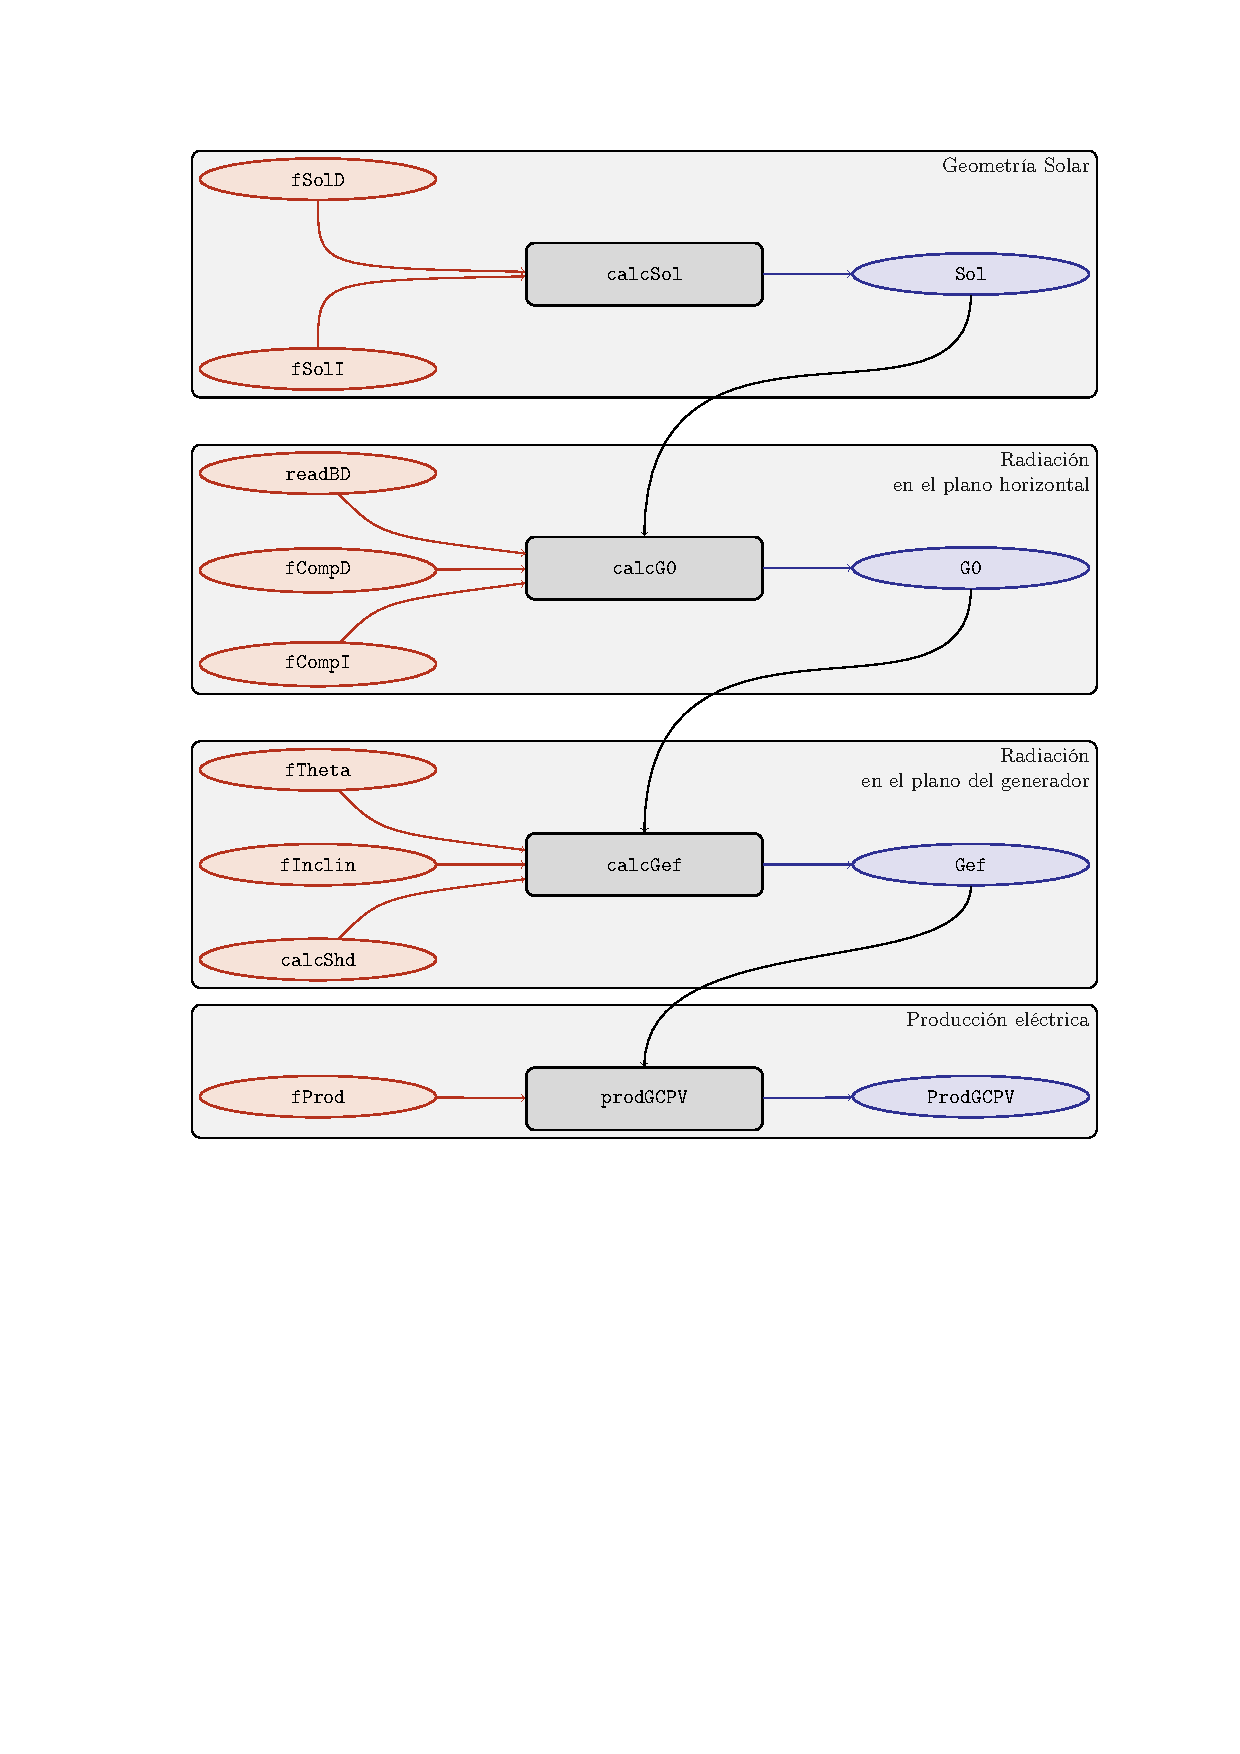
\includegraphics[keepaspectratio,width=0.8\textwidth,height=0.5\textheight]{figuras/procedure.pdf}
\caption{\label{fig:org79600e1}Proceso de cálculo de las funciones de \texttt{solaR2}}
\end{figure}
A la hora de estimar la producción, el programa sigue los siguientes procesos:
\section{Geometría solar}
\label{sec:org782662c}
\label{sec:geometria-solar}
Para calcular la geometría que definen las posiciones de la Tierra y el Sol, \texttt{solaR2} se vale de una función constructora, \texttt{calcSol} [\ref{subsec:calcsol}], la cual mediante las funciones \texttt{fSolD} [\ref{subsec:fsold}] y \texttt{fSolI} [\ref{subsec:fsoli}] cálcula todos los ángulos y componentes que caracterizan la geometría solar.
\begin{figure}[htbp]
\centering
\includegraphics[keepaspectratio,width=\textwidth,height=0.5\textheight]{figuras/calcSol.pdf}
\caption{Cálculo de la geometría solar mediante la función \texttt{calcSol}, la cual unifica las funciones \texttt{fSolD} y \texttt{fSolI} resultando en un objeto clase \texttt{Sol} el cual contiene toda la información geométrica necesaria para realizar las siguientes estimaciones. \label{fig:calcSol}}
\end{figure}

Como se puede ver en la figura \ref{fig:calcSol}, \texttt{calcSol} funcia gracias a las siguientes funciones:
\begin{itemize}
\item \texttt{fSolD}: la cual, a partir de la latitud (\(\phi\)), calcula la geometría a nivel diario, es decir, los ángulos y componentes que se pueden calcular en cada día independiente.

Estas son:
\begin{itemize}
\item Declinación (\(\delta\)): calculada a partir de la función \texttt{declination}\footnote{Todas las funciones mencionadas en este punto, se encuentran en el apartado \ref{subsec:utils-angles}.}.
\item Excentricidad (\(\epsilon_o\)): obtenida mediante la función \texttt{eccentricity}.
\item Ecuación del tiempo (\(EoT\)): obtenida mediante la función \texttt{eot}.
\item Ángulo del amanecer (\(\omega_s\)): calculada a partir de la función \texttt{sunrise}.
\item Irradiancia diaria extra-atmosférica (\(B_{0d}(0)\)): obtenida a paritr de la función \texttt{bo0d}.
\end{itemize}
\end{itemize}
\begin{lstlisting}[numbers=left,language=r,label= ,caption= ,captionpos=b]
lat <- 37.2
BTd <- fBTd(mode = 'prom')
solD <- fSolD(lat = lat, BTd = BTd)
show(solD)
\end{lstlisting}

\begin{verbatim}
Key: <Dates>
         Dates   lat        decl        eo           EoT        ws      Bo0d
        <IDat> <num>       <num>     <num>         <num>     <num>     <num>
 1: 2024-01-17  37.2 -0.36271754 1.0340422 -0.0455346238 -1.278593  4738.993
 2: 2024-02-14  37.2 -0.22850166 1.0259717 -0.0614793356 -1.393341  6137.388
 3: 2024-03-15  37.2 -0.03191616 1.0107943 -0.0368674274 -1.546560  8086.323
 4: 2024-04-15  37.2  0.17531794 0.9926547  0.0017482721 -1.705659  9921.357
 5: 2024-05-15  37.2  0.33246485 0.9775162  0.0143055938 -1.835976 11115.619
 6: 2024-06-10  37.2  0.40257826 0.9691480 -0.0007378952 -1.899934 11573.907
 7: 2024-07-18  37.2  0.36439367 0.9675489 -0.0263454380 -1.864521 11257.133
 8: 2024-08-18  37.2  0.22407398 0.9758022 -0.0111761118 -1.744657 10183.208
 9: 2024-09-18  37.2  0.02730595 0.9907919  0.0342189964 -1.591529  8508.642
10: 2024-10-19  37.2 -0.17900474 1.0088406  0.0689613044 -1.433019  6554.218
11: 2024-11-18  37.2 -0.33862399 1.0245012  0.0575423573 -1.300179  4951.750
12: 2024-12-13  37.2 -0.40478283 1.0328516  0.0158622941 -1.239567  4284.472
\end{verbatim}

Además, \texttt{fSolD} permite seleccionar el método de cáculo entre los propuestos por 4 autores diferentes (\texttt{cooper} \cite{Cooper1969}, \texttt{spencer} \cite{Spencer1971}, \texttt{strous} \cite{Strous2011}, \texttt{michalsky} \cite{Michalsky1988})(el valor por defecto es \texttt{michalsky}):
\begin{lstlisting}[numbers=left,language=r,label= ,caption= ,captionpos=b]
solD_cooper <- fSolD(lat = lat, BTd = BTd, method = 'cooper')
show(solD_cooper)
\end{lstlisting}

\begin{verbatim}
Key: <Dates>
         Dates   lat        decl        eo           EoT        ws      Bo0d
        <IDat> <num>       <num>     <num>         <num>     <num>     <num>
 1: 2024-01-17  37.2 -0.36506987 1.0315970 -0.0455346238 -1.276457  4702.617
 2: 2024-02-14  37.2 -0.23770977 1.0235842 -0.0614793356 -1.385835  6024.833
 3: 2024-03-15  37.2 -0.04219743 1.0091112 -0.0368674274 -1.538742  7968.679
 4: 2024-04-15  37.2  0.17074888 0.9917107  0.0017482721 -1.702053  9870.335
 5: 2024-05-15  37.2  0.33214647 0.9770196  0.0143055938 -1.835696 11107.378
 6: 2024-06-10  37.2  0.40292516 0.9690335 -0.0007378952 -1.900263 11575.213
 7: 2024-07-18  37.2  0.36346384 0.9684861 -0.0263454380 -1.863677 11260.684
 8: 2024-08-18  37.2  0.21721704 0.9778484 -0.0111761118 -1.739110 10144.635
 9: 2024-09-18  37.2  0.01056696 0.9933706  0.0342189964 -1.578817  8367.014
10: 2024-10-19  37.2 -0.19902155 1.0107363  0.0689613044 -1.417100  6356.454
11: 2024-11-18  37.2 -0.34965673 1.0247443  0.0575423573 -1.290358  4835.353
12: 2024-12-13  37.2 -0.40651987 1.0315970  0.0158622941 -1.237915  4260.830
\end{verbatim}

\begin{lstlisting}[numbers=left,language=r,label= ,caption= ,captionpos=b]
solD_spencer <- fSolD(lat = lat, BTd = BTd, method = 'spencer')
show(solD_spencer)
\end{lstlisting}

\begin{verbatim}
Key: <Dates>
         Dates   lat        decl        eo           EoT        ws      Bo0d
        <IDat> <num>       <num>     <num>         <num>     <num>     <num>
 1: 2024-01-17  37.2 -0.36483670 1.0340422 -0.0455346238 -1.276669  4716.264
 2: 2024-02-14  37.2 -0.23199205 1.0259717 -0.0614793356 -1.390501  6100.057
 3: 2024-03-15  37.2 -0.03563921 1.0107943 -0.0368674274 -1.543730  8048.574
 4: 2024-04-15  37.2  0.17171286 0.9926547  0.0017482721 -1.702813  9888.522
 5: 2024-05-15  37.2  0.33007088 0.9775162  0.0143055938 -1.833871 11096.093
 6: 2024-06-10  37.2  0.40208757 0.9691480 -0.0007378952 -1.899469 11570.124
 7: 2024-07-18  37.2  0.36657157 0.9675489 -0.0263454380 -1.866501 11274.319
 8: 2024-08-18  37.2  0.22748717 0.9758022 -0.0111761118 -1.747427 10212.886
 9: 2024-09-18  37.2  0.03143967 0.9907919  0.0342189964 -1.594670  8548.821
10: 2024-10-19  37.2 -0.17549393 1.0088406  0.0689613044 -1.435795  6590.939
11: 2024-11-18  37.2 -0.33679169 1.0245012  0.0575423573 -1.301800  4971.285
12: 2024-12-13  37.2 -0.40419949 1.0328516  0.0158622941 -1.240121  4290.674
\end{verbatim}

\begin{lstlisting}[numbers=left,language=r,label= ,caption= ,captionpos=b]
solD_strous <- fSolD(lat = lat, BTd = BTd, method = 'cooper')
show(solD_strous)
\end{lstlisting}

\begin{verbatim}
Key: <Dates>
         Dates   lat        decl        eo           EoT        ws      Bo0d
        <IDat> <num>       <num>     <num>         <num>     <num>     <num>
 1: 2024-01-17  37.2 -0.36506987 1.0315970 -0.0455346238 -1.276457  4702.617
 2: 2024-02-14  37.2 -0.23770977 1.0235842 -0.0614793356 -1.385835  6024.833
 3: 2024-03-15  37.2 -0.04219743 1.0091112 -0.0368674274 -1.538742  7968.679
 4: 2024-04-15  37.2  0.17074888 0.9917107  0.0017482721 -1.702053  9870.335
 5: 2024-05-15  37.2  0.33214647 0.9770196  0.0143055938 -1.835696 11107.378
 6: 2024-06-10  37.2  0.40292516 0.9690335 -0.0007378952 -1.900263 11575.213
 7: 2024-07-18  37.2  0.36346384 0.9684861 -0.0263454380 -1.863677 11260.684
 8: 2024-08-18  37.2  0.21721704 0.9778484 -0.0111761118 -1.739110 10144.635
 9: 2024-09-18  37.2  0.01056696 0.9933706  0.0342189964 -1.578817  8367.014
10: 2024-10-19  37.2 -0.19902155 1.0107363  0.0689613044 -1.417100  6356.454
11: 2024-11-18  37.2 -0.34965673 1.0247443  0.0575423573 -1.290358  4835.353
12: 2024-12-13  37.2 -0.40651987 1.0315970  0.0158622941 -1.237915  4260.830
\end{verbatim}

\begin{itemize}
\item \texttt{fSolI}: toma los resultados obtenidos en \texttt{fSolD} y calcula la geometría a nivel intradiario, es decir, aquella que se puede calcular en unidades de tiempo menores a los días.
Estas son:
\begin{itemize}
\item La hora solar o tiempo solar verdadero (\(\omega\)): calculada a partir de la función \texttt{sunHour}.
\item Los momentos del día en los que es de noche (\(night\)): calculada a partir del resultado anterior y de el ángulo del amanecer (cálculada en \texttt{fSolD})\footnote{Cuando la hora solar verdadera excede los ángulos en los que amanece y anochece (\(|\omega|>=|\omega_s|\)), el Sol queda por debajo de la línea del horizonte, por lo que es de noche.}.
\item El coseno del ángulo cenital solar (\(cos(\theta_{zs})\)): obtenida a partir de la función \texttt{zenith}.
\item La altura solar (\(\gamma_s\)): obtenida a partir del resultado anterior\footnote{\(\gamma_s=asin(cos(\theta_s))\).}.
\item El ángulo acimutal solar (\(\theta_{zs}\)): calculada mediante la función \texttt{azimuth}.
\item La irradiancia extra-atmosférica (\(B_0(0)\)): calculada mediante el coseno del ángulo cenital, la constante solar (\(B_0\)) y la excentridad (cálculada en \texttt{fSolD}) [ecuación \ref{eq:irrad_horiz}].
\end{itemize}
\end{itemize}
\begin{lstlisting}[numbers=left,language=r,label= ,caption= ,captionpos=b]
solI <- fSolI(solD = solD[1], sample = 'hour') #Computo solo un día a fin mejorar la visualización
show(solI)
\end{lstlisting}

\begin{verbatim}
Index: <night>
                  Dates   lat           w  night      cosThzS          AlS         AzS       Bo0
                 <POSc> <num>       <num> <lgcl>        <num>        <num>       <num>     <num>
 1: 2024-01-17 00:00:00  37.2  3.09905026   TRUE -0.958552332 -1.281876984  3.00157749   0.00000
 2: 2024-01-17 01:00:00  37.2 -2.92239722   TRUE -0.941407376 -1.226779122 -2.49462689   0.00000
 3: 2024-01-17 02:00:00  37.2 -2.66065932   TRUE -0.874749489 -1.064918604 -2.03862388   0.00000
 4: 2024-01-17 03:00:00  37.2 -2.39892132   TRUE -0.763119126 -0.868125900 -1.77932134   0.00000
 5: 2024-01-17 04:00:00  37.2 -2.13718324   TRUE -0.614120126 -0.661270606 -1.59701536   0.00000
 6: 2024-01-17 05:00:00  37.2 -1.87544507   TRUE -0.437901763 -0.453263434 -1.44469585   0.00000
 7: 2024-01-17 06:00:00  37.2 -1.61370681   TRUE -0.246467423 -0.249033534 -1.30093496   0.00000
 8: 2024-01-17 07:00:00  37.2 -1.35196846   TRUE -0.052856976 -0.052881619 -1.15283370   0.00000
 9: 2024-01-17 08:00:00  37.2 -1.09023003  FALSE  0.129741461  0.130108233 -0.99014548 183.39419
10: 2024-01-17 09:00:00  37.2 -0.82849151  FALSE  0.288889848  0.293067041 -0.80329847 408.35612
11: 2024-01-17 10:00:00  37.2 -0.56675290  FALSE  0.413747472  0.426566560 -0.58400587 584.84684
12: 2024-01-17 11:00:00  37.2 -0.30501420  FALSE  0.495809380  0.518766586 -0.32921922 700.84427
13: 2024-01-17 12:00:00  37.2 -0.04327541  FALSE  0.529485721  0.557994217 -0.04769723 748.44699
14: 2024-01-17 13:00:00  37.2  0.21846346  FALSE  0.512482515  0.538073327  0.23821864 724.41235
15: 2024-01-17 14:00:00  37.2  0.48020243  FALSE  0.445957919  0.462244212  0.50355560 630.37745
16: 2024-01-17 15:00:00  37.2  0.74194148  FALSE  0.334443348  0.341014503  0.73469016 472.74762
17: 2024-01-17 16:00:00  37.2  1.00368062  FALSE  0.185534810  0.186616094  0.93148844 262.26008
18: 2024-01-17 17:00:00  37.2  1.26541985  FALSE  0.009375501  0.009375638  1.10112996  13.25261
19: 2024-01-17 18:00:00  37.2  1.52715917   TRUE -0.182035120 -0.183055757  1.25297092   0.00000
20: 2024-01-17 19:00:00  37.2  1.78889857   TRUE -0.375658695 -0.385107424  1.39694027   0.00000
21: 2024-01-17 20:00:00  37.2  2.05063807   TRUE -0.558306105 -0.592342658  1.54466726   0.00000
22: 2024-01-17 21:00:00  37.2  2.31237766   TRUE -0.717535874 -0.800258081  1.71368519   0.00000
23: 2024-01-17 22:00:00  37.2  2.57411733   TRUE -0.842501657 -1.001910427  1.93928567   0.00000
24: 2024-01-17 23:00:00  37.2  2.83585709   TRUE -0.924691065 -1.180223341  2.30977400   0.00000
                  Dates   lat           w  night      cosThzS          AlS         AzS       Bo0
\end{verbatim}

Además, como los datos nocturnos aportan poco a los cálculos que atañen a este proyecto, \texttt{fSolI} presenta la posibilidad de eliminar estos datos con el argumento \texttt{keep.night}.
\begin{lstlisting}[numbers=left,language=r,label= ,caption= ,captionpos=b]
solI_nigth <- fSolI(solD = solD[1], sample = 'hour', keep.night = FALSE)
show(solI_nigth)
\end{lstlisting}

\begin{verbatim}
                  Dates   lat           w  night     cosThzS         AlS         AzS       Bo0
                 <POSc> <num>       <num> <lgcl>       <num>       <num>       <num>     <num>
 1: 2024-01-17 08:00:00  37.2 -1.09023003  FALSE 0.129741461 0.130108233 -0.99014548 183.39419
 2: 2024-01-17 09:00:00  37.2 -0.82849151  FALSE 0.288889848 0.293067041 -0.80329847 408.35612
 3: 2024-01-17 10:00:00  37.2 -0.56675290  FALSE 0.413747472 0.426566560 -0.58400587 584.84684
 4: 2024-01-17 11:00:00  37.2 -0.30501420  FALSE 0.495809380 0.518766586 -0.32921922 700.84427
 5: 2024-01-17 12:00:00  37.2 -0.04327541  FALSE 0.529485721 0.557994217 -0.04769723 748.44699
 6: 2024-01-17 13:00:00  37.2  0.21846346  FALSE 0.512482515 0.538073327  0.23821864 724.41235
 7: 2024-01-17 14:00:00  37.2  0.48020243  FALSE 0.445957919 0.462244212  0.50355560 630.37745
 8: 2024-01-17 15:00:00  37.2  0.74194148  FALSE 0.334443348 0.341014503  0.73469016 472.74762
 9: 2024-01-17 16:00:00  37.2  1.00368062  FALSE 0.185534810 0.186616094  0.93148844 262.26008
10: 2024-01-17 17:00:00  37.2  1.26541985  FALSE 0.009375501 0.009375638  1.10112996  13.25261
\end{verbatim}

Aparte, en vez de identificar el intervalo intradiario (con el argumento \texttt{sample}), se puede dar directamente la base temporal intradiaria.
\begin{lstlisting}[numbers=left,language=r,label= ,caption= ,captionpos=b]
BTi <- fBTi(BTd, sample = 'hour')
solI_BTi <- fSolI(solD, BTi = BTi)
show(solI_BTi)
\end{lstlisting}

\begin{verbatim}
Index: <night>
                   Dates   lat         w  night    cosThzS        AlS       AzS   Bo0
                  <POSc> <num>     <num> <lgcl>      <num>      <num>     <num> <num>
  1: 2024-01-17 00:00:00  37.2  3.099050   TRUE -0.9585523 -1.2818770  3.001577     0
  2: 2024-01-17 01:00:00  37.2 -2.922397   TRUE -0.9414074 -1.2267791 -2.494627     0
  3: 2024-01-17 02:00:00  37.2 -2.660659   TRUE -0.8747495 -1.0649186 -2.038624     0
  4: 2024-01-17 03:00:00  37.2 -2.398921   TRUE -0.7631191 -0.8681259 -1.779321     0
  5: 2024-01-17 04:00:00  37.2 -2.137183   TRUE -0.6141201 -0.6612706 -1.597015     0
 ---                                                                                 
284: 2024-12-13 19:00:00  37.2  1.856445   TRUE -0.4444110 -0.4605166  1.394524     0
285: 2024-12-13 20:00:00  37.2  2.118158   TRUE -0.6191456 -0.6676542  1.539641     0
286: 2024-12-13 21:00:00  37.2  2.379871   TRUE -0.7679298 -0.8756029  1.709361     0
287: 2024-12-13 22:00:00  37.2  2.641583   TRUE -0.8806309 -1.0771921  1.946876     0
288: 2024-12-13 23:00:00  37.2  2.903296   TRUE -0.9495736 -1.2518732  2.377338     0
\end{verbatim}

También, se puede indicar que no realice las correcciones de la ecuación del tiempo.
\begin{lstlisting}[numbers=left,language=r,label= ,caption= ,captionpos=b]
solI_EoT <- fSolI(solD = solD, BTi = BTi, EoT = FALSE)
show(solI_EoT)
\end{lstlisting}

\begin{verbatim}
Index: <night>
                   Dates   lat         w  night    cosThzS        AlS       AzS   Bo0
                  <POSc> <num>     <num> <lgcl>      <num>      <num>     <num> <num>
  1: 2024-01-17 00:00:00  37.2  3.099050   TRUE -0.9585523 -1.2818770  3.001577     0
  2: 2024-01-17 01:00:00  37.2 -2.922397   TRUE -0.9414074 -1.2267791 -2.494627     0
  3: 2024-01-17 02:00:00  37.2 -2.660659   TRUE -0.8747495 -1.0649186 -2.038624     0
  4: 2024-01-17 03:00:00  37.2 -2.398921   TRUE -0.7631191 -0.8681259 -1.779321     0
  5: 2024-01-17 04:00:00  37.2 -2.137183   TRUE -0.6141201 -0.6612706 -1.597015     0
 ---                                                                                 
284: 2024-12-13 19:00:00  37.2  1.856445   TRUE -0.4444110 -0.4605166  1.394524     0
285: 2024-12-13 20:00:00  37.2  2.118158   TRUE -0.6191456 -0.6676542  1.539641     0
286: 2024-12-13 21:00:00  37.2  2.379871   TRUE -0.7679298 -0.8756029  1.709361     0
287: 2024-12-13 22:00:00  37.2  2.641583   TRUE -0.8806309 -1.0771921  1.946876     0
288: 2024-12-13 23:00:00  37.2  2.903296   TRUE -0.9495736 -1.2518732  2.377338     0
\end{verbatim}

Finalmente, estas dos funciones, como se muestra en la figura \ref{fig:calcSol}, convergen en la función \texttt{calcSol}, dando como resultado un objeto de clase \texttt{Sol}. Este objeto muestra un resumen de ambos elementos junto con la latitud de los cálculos.
\begin{lstlisting}[numbers=left,language=r,label= ,caption= ,captionpos=b]
sol <- calcSol(lat = lat, BTd = BTd, sample = 'hour')
show(sol)
\end{lstlisting}

\begin{verbatim}
Object of class Sol 

Latitude:  37.2 degrees

Daily values:
     Dates                 decl                 eo              EoT                   ws        
 Min.   :2024-01-17   Min.   :-0.404783   Min.   :0.9675   Min.   :-0.0614793   Min.   :-1.900  
 1st Qu.:2024-04-07   1st Qu.:-0.256032   1st Qu.:0.9771   1st Qu.:-0.0289759   1st Qu.:-1.767  
 Median :2024-06-29   Median :-0.002305   Median :1.0007   Median : 0.0005052   Median :-1.569  
 Mean   :2024-07-01   Mean   :-0.001618   Mean   :1.0009   Mean   : 0.0008748   Mean   :-1.569  
 3rd Qu.:2024-09-25   3rd Qu.: 0.251172   3rd Qu.:1.0249   3rd Qu.: 0.0204515   3rd Qu.:-1.370  
 Max.   :2024-12-13   Max.   : 0.402578   Max.   :1.0340   Max.   : 0.0689613   Max.   :-1.240  
      Bo0d      
 Min.   : 4284  
 1st Qu.: 5841  
 Median : 8297  
 Mean   : 8109  
 3rd Qu.:10416  
 Max.   :11574  

Intradaily values: 
     Dates                           w                night            cosThzS          
 Min.   :2024-01-17 00:00:00   Min.   :-3.1393050   Mode :logical   Min.   :-0.9700256  
 1st Qu.:2024-04-07 11:45:00   1st Qu.:-1.5692285   FALSE:145       1st Qu.:-0.5004531  
 Median :2024-06-29 11:30:00   Median : 0.0010871   TRUE :143       Median : 0.0062923  
 Mean   :2024-07-01 15:30:00   Mean   : 0.0009975                   Mean   :-0.0009523  
 3rd Qu.:2024-09-26 11:15:00   3rd Qu.: 1.5716412                   3rd Qu.: 0.5007129  
 Max.   :2024-12-13 23:00:00   Max.   : 3.1413972                   Max.   : 0.9697262  
      AlS                 AzS                 Bo0          
 Min.   :-1.325336   Min.   :-3.139169   Min.   :   0.000  
 1st Qu.:-0.524130   1st Qu.:-1.570722   1st Qu.:   0.000  
 Median : 0.006292   Median : 0.003834   Median :   8.748  
 Mean   :-0.001202   Mean   : 0.001011   Mean   : 337.752  
 3rd Qu.: 0.524433   3rd Qu.: 1.555342   3rd Qu.: 698.153  
 Max.   : 1.324107   Max.   : 3.141331   Max.   :1284.718
\end{verbatim}

\section{Datos meteorológicos}
\label{sec:org3a06ee8}
\label{sec:datos-meteorologicos}
Para el procesamiento de datos meteorologicos, \texttt{solaR2} provee una serie de funciones\footnote{Las funciones comentadas en este apartado, se recogen en la sección \ref{subsec:meteoreaders}} que son capaces de leer todo tipo de datos. Estos datos se procesan y se almacenan en un objeto de tipo \texttt{Meteo} tal y como se ve en la figura \ref{fig:meteo}. Estas funciones son:
\begin{figure}[htbp]
\centering
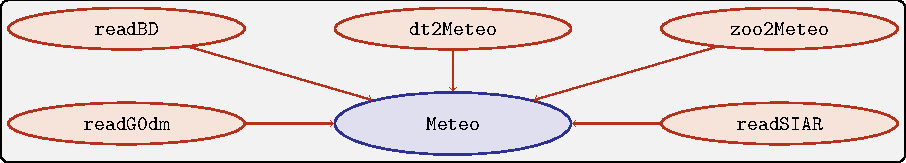
\includegraphics[keepaspectratio,width=\textwidth,height=0.5\textheight]{figuras/meteo.pdf}
\caption{Los datos meteorologicas se pueden leer mediante las funciones \texttt{readG0dm}, \texttt{readBD}, \texttt{dt2Meteo}, \texttt{zoo2Meteo} y \texttt{readSIAR} las cuales procesan estos datos y los almacenan en un objeto de clase \texttt{Meteo}. \label{fig:meteo}}
\end{figure}
\begin{itemize}
\item \texttt{readG0dm}: Esta función construye un objeto \texttt{Meteo} a partir de 12 valores de medias mensuales de irradiación.
\end{itemize}
\begin{lstlisting}[numbers=left,language=r,label= ,caption= ,captionpos=b]
G0dm = c(2.766,3.491,4.494,5.912,6.989,7.742,
         7.919,7.027,5.369,3.562,2.814,2.179) * 1000;
Ta = c(10, 14.1, 15.6, 17.2, 19.3, 21.2,
       28.4, 29.9, 24.3, 18.2, 17.2, 15.2)
BD <- readG0dm(G0dm = G0dm, Ta = Ta, lat = 37.2)
show(BD)
\end{lstlisting}

\begin{verbatim}
Object of class  Meteo 

Source of meteorological information: prom- 
Latitude of source:  37.2 degrees

Meteorological Data:
     Dates                 G0d             Ta       
 Min.   :2024-01-17   Min.   :2179   Min.   :10.00  
 1st Qu.:2024-04-07   1st Qu.:3322   1st Qu.:15.50  
 Median :2024-06-29   Median :4932   Median :17.70  
 Mean   :2024-07-01   Mean   :5022   Mean   :19.22  
 3rd Qu.:2024-09-25   3rd Qu.:6998   3rd Qu.:21.98  
 Max.   :2024-12-13   Max.   :7919   Max.   :29.90
\end{verbatim}

\begin{itemize}
\item \texttt{readBD}: Esta familia de funciones puede leer ficheros de datos y transformarlos en un objeto de clase \texttt{Meteo}. Se dividen en:
\begin{itemize}
\item \texttt{readBDd}: Procesa datos meteorológicos de tipo diarios.
\end{itemize}
\begin{lstlisting}[numbers=left,language=r,label= ,caption= ,captionpos=b]
## Se utiliza un archivo alojado en el
## github del tutor de este proyecto 
myURL <-"https://raw.githubusercontent.com/oscarperpinan/R/master/data/aranjuez.csv"
download.file(myURL, 'data/aranjuez.csv', quiet = TRUE)
BDd <- readBDd(file = 'data/aranjuez.csv', lat = lat,
               format = '%Y-%m-%d', header = TRUE,
               fill = TRUE, dec = '.', sep = ',', dates.col = '',
               ta.col = 'TempAvg', g0.col = 'Radiation', keep.cols = TRUE)
show(BDd)
\end{lstlisting}

\begin{verbatim}
Object of class  Meteo 

Source of meteorological information: bd-data/aranjuez.csv 
Latitude of source:  37.2 degrees

Meteorological Data:
     Dates                  G0               Ta            TempMin           TempMax      
 Min.   :2004-01-01   Min.   : 0.277   Min.   :-5.309   Min.   :-12.980   Min.   :-2.362  
 1st Qu.:2005-12-29   1st Qu.: 9.370   1st Qu.: 7.692   1st Qu.:  1.515   1st Qu.:14.530  
 Median :2008-01-09   Median :16.660   Median :13.810   Median :  7.170   Median :21.670  
 Mean   :2008-01-03   Mean   :16.742   Mean   :14.405   Mean   :  6.888   Mean   :22.531  
 3rd Qu.:2010-01-02   3rd Qu.:24.650   3rd Qu.:21.615   3rd Qu.: 12.590   3rd Qu.:30.875  
 Max.   :2011-12-31   Max.   :32.740   Max.   :30.680   Max.   : 22.710   Max.   :41.910  
		      NA's   :13                        NA's   :4                         
    HumidAvg         HumidMax         WindAvg         WindMax            Rain              ET       
 Min.   : 19.89   Min.   : 35.88   Min.   :0.251   Min.   : 0.000   Min.   : 0.000   Min.   :0.000  
 1st Qu.: 47.04   1st Qu.: 81.60   1st Qu.:0.667   1st Qu.: 3.783   1st Qu.: 0.000   1st Qu.:1.168  
 Median : 62.58   Median : 90.90   Median :0.920   Median : 5.027   Median : 0.000   Median :2.758  
 Mean   : 62.16   Mean   : 87.22   Mean   :1.174   Mean   : 5.208   Mean   : 1.094   Mean   :3.091  
 3rd Qu.: 77.38   3rd Qu.: 94.90   3rd Qu.:1.431   3rd Qu.: 6.537   3rd Qu.: 0.200   3rd Qu.:4.926  
 Max.   :100.00   Max.   :100.00   Max.   :8.260   Max.   :10.000   Max.   :49.730   Max.   :8.564  
		  NA's   :13       NA's   :8       NA's   :128      NA's   :4        NA's   :18
\end{verbatim}

\begin{itemize}
\item \texttt{readBDi}: Procesa datos meteorológicos de tipo intradiarios.
\end{itemize}
\begin{lstlisting}[numbers=left,language=r,label= ,caption= ,captionpos=b]
myURL <- "https://raw.githubusercontent.com/oscarperpinan/R/master/data/NREL-Hawaii.csv"
download.file(myURL, 'data/NREL-Hawaii.csv', quiet = TRUE)
BDi <- readBDi(file = 'data/NREL-Hawaii.csv', lat = 19,
               format = "%d/%m/%Y %H:%M", header = TRUE,
               fill = TRUE, dec = '.', sep = ',',
               dates.col = 'DATE', times.col = 'HST',
               ta.col = 'Air Temperature [deg C]',
               g0.col = 'Global Horizontal [W/m^2]',
               keep.cols = TRUE)
show(BDi)
\end{lstlisting}

\begin{verbatim}
Object of class  Meteo 

Source of meteorological information: bdI-data/NREL-Hawaii.csv 
Latitude of source:  19 degrees

Meteorological Data:
     Dates                              G0                  Ta        Direct Normal [W/m^2]
 Min.   :2010-01-11 06:32:00.00   Min.   :   0.4769   Min.   :13.42   Min.   :  0.0        
 1st Qu.:2010-03-11 17:37:45.00   1st Qu.: 147.4328   1st Qu.:22.76   1st Qu.:  0.0        
 Median :2010-06-11 17:32:30.00   Median : 300.6510   Median :24.15   Median :270.3        
 Mean   :2010-06-26 11:55:22.63   Mean   : 370.5293   Mean   :23.64   Mean   :356.6        
 3rd Qu.:2010-09-11 17:34:15.00   3rd Qu.: 585.7402   3rd Qu.:25.24   3rd Qu.:715.2        
 Max.   :2010-12-11 17:46:00.00   Max.   :1172.3000   Max.   :28.12   Max.   :943.0        
 NA's   :4660                                                                              
 Diffuse Horizontal [W/m^2]
 Min.   :  0.4769          
 1st Qu.: 78.4636          
 Median :152.9320          
 Mean   :171.7706          
 3rd Qu.:246.3193          
 Max.   :586.3600
\end{verbatim}

\item \texttt{dt2Meteo}: Transforma un \texttt{data.table} o \texttt{data.frame} en un objeto de clase \texttt{Meteo}.
\end{itemize}
\begin{lstlisting}[numbers=left,language=r,label= ,caption= ,captionpos=b]
data(helios)
names(helios) <- c('Dates', 'G0d', 'TempMax', 'TempMin')
helios_meteo <- dt2Meteo(file = helios, lat = 40, type = 'bd')
show(helios_meteo)
\end{lstlisting}

\begin{verbatim}
Object of class  Meteo 

Source of meteorological information: bd-data.frame 
Latitude of source:  40 degrees

Meteorological Data:
     Dates                             G0d             TempMin           TempMax     
 Min.   :2009-01-01 00:00:00.00   Min.   :  325.6   Min.   :-37.500   Min.   : 1.41  
 1st Qu.:2009-04-08 12:00:00.00   1st Qu.: 2523.2   1st Qu.:  1.950   1st Qu.:14.41  
 Median :2009-07-07 00:00:00.00   Median : 4745.7   Median :  7.910   Median :23.16  
 Mean   :2009-07-04 21:29:54.93   Mean   : 4812.0   Mean   :  5.323   Mean   :22.59  
 3rd Qu.:2009-10-03 12:00:00.00   3rd Qu.: 7139.5   3rd Qu.: 15.105   3rd Qu.:31.06  
 Max.   :2009-12-31 00:00:00.00   Max.   :11253.9   Max.   : 24.800   Max.   :38.04  
       Ta         
 Min.   :-23.049  
 1st Qu.:  7.008  
 Median : 12.055  
 Mean   : 10.944  
 3rd Qu.: 19.472  
 Max.   : 28.619
\end{verbatim}

\begin{itemize}
\item \texttt{zoo2Meteo}: Transforma un objeto de clase \texttt{zoo}\footnote{Pese a que este proyecto trate de ``desligarse'' del paquete \texttt{zoo}, sigue siendo un paquete muy extendido. Por lo que es interesante tener una función así para que los usuarios tengan una mayor flexibilidad.} en un objeto de clase \texttt{Meteo}.
\end{itemize}
\begin{lstlisting}[numbers=left,language=r,label= ,caption= ,captionpos=b]
library(zoo)
bd_zoo <- read.csv.zoo('data/aranjuez.csv')
BD_zoo <- zoo2Meteo(file = bd_zoo, lat = 40)
show(BD_zoo)
\end{lstlisting}

\begin{verbatim}
Object of class  Meteo 

Source of meteorological information: bd-zoo-bd_zoo 
Latitude of source:  40 degrees

Meteorological Data:
    TempAvg          TempMax          TempMin           HumidAvg         HumidMax         WindAvg     
 Min.   :-5.309   Min.   :-2.362   Min.   :-12.980   Min.   : 19.89   Min.   : 35.88   Min.   :0.251  
 1st Qu.: 7.692   1st Qu.:14.530   1st Qu.:  1.515   1st Qu.: 47.04   1st Qu.: 81.60   1st Qu.:0.667  
 Median :13.810   Median :21.670   Median :  7.170   Median : 62.58   Median : 90.90   Median :0.920  
 Mean   :14.405   Mean   :22.531   Mean   :  6.888   Mean   : 62.16   Mean   : 87.22   Mean   :1.174  
 3rd Qu.:21.615   3rd Qu.:30.875   3rd Qu.: 12.590   3rd Qu.: 77.38   3rd Qu.: 94.90   3rd Qu.:1.431  
 Max.   :30.680   Max.   :41.910   Max.   : 22.710   Max.   :100.00   Max.   :100.00   Max.   :8.260  
                                   NA's   :4                          NA's   :13       NA's   :8      
    WindMax            Rain          Radiation            ET       
 Min.   : 0.000   Min.   : 0.000   Min.   : 0.277   Min.   :0.000  
 1st Qu.: 3.783   1st Qu.: 0.000   1st Qu.: 9.370   1st Qu.:1.168  
 Median : 5.027   Median : 0.000   Median :16.660   Median :2.758  
 Mean   : 5.208   Mean   : 1.094   Mean   :16.742   Mean   :3.091  
 3rd Qu.: 6.537   3rd Qu.: 0.200   3rd Qu.:24.650   3rd Qu.:4.926  
 Max.   :10.000   Max.   :49.730   Max.   :32.740   Max.   :8.564  
 NA's   :128      NA's   :4        NA's   :13       NA's   :18
\end{verbatim}

\begin{itemize}
\item \texttt{readSIAR}: Esta función es capaz de extraer información de la red SIAR y transformarlo en un objeto de clase \texttt{Meteo}.
\end{itemize}
\begin{lstlisting}[numbers=left,language=r,label= ,caption= ,captionpos=b]
library(httr2)
library(jsonlite)
bd_SIAR <- readSIAR(Lat = 40.40596822621351, Lon = -3.70038308516172,
                    ## Ubicación de la Escuela Técnica Superior
                    ## de Ingeniería y Diseño Industrial (ETSIDI)
                    inicio = '2023-09-01', final = '2024-08-01',
                    tipo = 'Mensuales', n_est = 3)
show(bd_SIAR)
\end{lstlisting}

\begin{verbatim}
Object of class  Meteo 

Source of meteorological information: prom-https://servicio.mapama.gob.es 
  -Estaciones: Center: Finca experimental(M01), Arganda(M02), San Martín de la Vega(M05) 
Latitude of source:  40.4 degrees

Meteorological Data:
     Dates                          G0d             Ta            TempMin           TempMax     
 Min.   :2023-09-18 00:00:00   Min.   :1860   Min.   : 5.318   Min.   :-4.6513   Min.   :15.34  
 1st Qu.:2023-12-06 18:00:00   1st Qu.:2744   1st Qu.: 9.857   1st Qu.:-2.1466   1st Qu.:21.12  
 Median :2024-02-29 00:00:00   Median :4052   Median :14.890   Median : 0.3663   Median :31.01  
 Mean   :2024-03-01 04:00:00   Mean   :4502   Mean   :15.307   Mean   : 2.4225   Mean   :29.41  
 3rd Qu.:2024-05-21 12:00:00   3rd Qu.:6549   3rd Qu.:20.047   3rd Qu.: 7.1506   3rd Qu.:35.47  
 Max.   :2024-08-18 00:00:00   Max.   :7608   Max.   :27.069   Max.   :12.6082   Max.   :40.70
\end{verbatim}

Esta función tiene dos argumentos importantes:
\begin{itemize}
\item \texttt{tipo}: La API SIAR\footnote{La API (Interfaz de Programación de Aplicaciones) que se usa para la función \texttt{readSIAR} está proporcionada por la propia red SIAR \cite{siar23}.} permite tener 4 tipos de registros: \texttt{Mensuales}, \texttt{Semanales}, \texttt{Diarios} y \texttt{Horarios}.
\item \texttt{n\_est}: Con este argumento, la función es capaz de localizar el número seleccionado de estaciones más proximas a la ubicación dada, y obtener los datos individuales de cada una de ellas. Una vez obtenidos estos datos realiza una interpolación de distancia inversa ponderada (IDW) y entrega un solo resultado. Es importante añadir que la API SIAR tiene una limitación a la solicitud de registros que se le hace cada minuto, por lo que esta función cuenta con un comprobante para impedir que el usuario exceda este límite.
\end{itemize}

\section{Radiación en el plano horizontal}
\label{sec:org891bcda}
\label{sec:radiacion-plano-horizontal}
Una vez se ha calculado la geometría solar (sección \ref{sec:geometria-solar}) y se han procesado los datos meteorológicos (sección \ref{sec:datos-meteorologicos}), es necesario calcular la radiación en el plano horizontal. Para ello, \texttt{solaR2} cuenta con la función \texttt{calcG0} [\ref{subsec:calcg0}] la cual mediante las funciones \texttt{fCompD} [\ref{subsec:fcompd}] y \texttt{fCompI} [\ref{subsec:fcompi}] procesan los objetos de clase \texttt{Sol} y clase \texttt{Meteo} para dar un objeto de tipo \texttt{G0}.

Como se puede ver en la figura \ref{fig:calcg0}, \texttt{calcG0} funciona gracias a las siguientes funciones:
\begin{figure}[htbp]
\centering
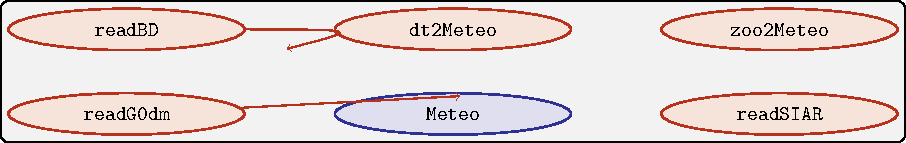
\includegraphics[keepaspectratio,width=\textwidth,height=0.5\textheight]{figuras/calcg0.pdf}
\caption{Cálculo de la radiación incidente en el plano horizontal mediante la función \texttt{calcG0}, la cual procesa un objeto clase \texttt{Sol} y otro clase \texttt{Meteo} mediante las funciones \texttt{fCompD} y \texttt{fCompI} resultando en un objeto clase \texttt{G0}. :\label{fig:calcg0}}
\end{figure}
\begin{itemize}
\item \texttt{fCompD}: La cual calcula todas las componentes de la irradiación diaria en una superficie horizontal mediante regresiones entre los parámetros del índice de claridad y la fracción difusa.
Para ello se pueden usar varias correlaciones dependiendo del tipo de datos:
\begin{itemize}
\item Mensuales:
\end{itemize}
\begin{lstlisting}[numbers=left,language=r,label= ,caption= ,captionpos=b]
lat <- 37.2
BTd <- fBTd(mode = 'prom')
solD <- fSolD(lat, BTd)
G0d <- c(2.766,3.491,4.494,5.912,6.989,7.742,7.919,7.027,5.369,3.562,2.814,2.179) * 1000
compD_page <- fCompD(sol = solD, G0d = G0d, corr = "Page")
compD_page
\end{lstlisting}

\begin{verbatim}
Key: <Dates>
	 Dates        Fd        Kt   G0d      D0d      B0d
	<POSc>     <num>     <num> <num>    <num>    <num>
 1: 2024-01-17 0.3404548 0.5836683  2766  941.698 1824.302
 2: 2024-02-14 0.3572461 0.5688088  3491 1247.146 2243.854
 3: 2024-03-15 0.3719989 0.5557532  4494 1671.763 2822.237
 4: 2024-04-15 0.3266485 0.5958862  5912 1931.146 3980.854
 5: 2024-05-15 0.2895069 0.6287549  6989 2023.364 4965.636
 6: 2024-06-10 0.2441221 0.6689185  7742 1889.994 5852.006
 7: 2024-07-18 0.2050844 0.7034651  7919 1624.064 6294.936
 8: 2024-08-18 0.2202349 0.6900576  7027 1547.591 5479.409
 9: 2024-09-18 0.2869638 0.6310055  5369 1540.708 3828.292
10: 2024-10-19 0.3858825 0.5434669  3562 1374.513 2187.487
11: 2024-11-18 0.3578392 0.5682839  2814 1006.959 1807.041
12: 2024-12-13 0.4253038 0.5085807  2179  926.737 1252.263
\end{verbatim}

\begin{lstlisting}[numbers=left,language=r,label= ,caption= ,captionpos=b]
compD_lj <- fCompD(sol = solD, G0d = G0d, corr = "LJ")
compD_lj
\end{lstlisting}

\begin{verbatim}
Key: <Dates>
	 Dates        Fd        Kt   G0d       D0d      B0d
	<POSc>     <num>     <num> <num>     <num>    <num>
 1: 2024-01-17 0.3058193 0.5836683  2766  845.8961 1920.104
 2: 2024-02-14 0.3169470 0.5688088  3491 1106.4621 2384.538
 3: 2024-03-15 0.3268047 0.5557532  4494 1468.6603 3025.340
 4: 2024-04-15 0.2967018 0.5958862  5912 1754.1011 4157.899
 5: 2024-05-15 0.2720419 0.6287549  6989 1901.3006 5087.699
 6: 2024-06-10 0.2408700 0.6689185  7742 1864.8154 5877.185
 7: 2024-07-18 0.2152460 0.7034651  7919 1704.5331 6214.467
 8: 2024-08-18 0.2236251 0.6900576  7027 1571.4138 5455.586
 9: 2024-09-18 0.2703347 0.6310055  5369 1451.4268 3917.573
10: 2024-10-19 0.3361895 0.5434669  3562 1197.5071 2364.493
11: 2024-11-18 0.3173415 0.5682839  2814  892.9990 1921.001
12: 2024-12-13 0.3637158 0.5085807  2179  792.5367 1386.463
\end{verbatim}

\begin{itemize}
\item Diarios:
\end{itemize}
\begin{lstlisting}[numbers=left,language=r,label= ,caption= ,captionpos=b]
G0d <- readSIAR(Lat = 40.40596822621351, Lon =-3.70038308516172,
                inicio = '2024-07-15', final = '2024-08-01',
                tipo = 'Diarios', n_est = 3)
sol <- calcSol(lat, BTd = indexD(G0d))
compD_cpr <- fCompD(sol = sol, G0d = G0d, corr = "CPR")
compD_cpr
\end{lstlisting}

\begin{verbatim}
Key: <Dates>
	 Dates        Fd        Kt      G0d      D0d      B0d
	<POSc>     <num>     <num>    <num>    <num>    <num>
 1: 2024-07-15 0.2833125 0.6798139 7697.945 2180.924 5517.021
 2: 2024-07-16 0.2597185 0.7000272 7911.858 2054.856 5857.002
 3: 2024-07-17 0.2815044 0.6812283 7684.293 2163.163 5521.131
 4: 2024-07-18 0.6627754 0.4674993 5262.702 3487.989 1774.713
 5: 2024-07-19 0.2595844 0.7001561 7865.166 2041.675 5823.491
 6: 2024-07-20 0.2594075 0.7003266 7849.961 2036.339 5813.622
 7: 2024-07-21 0.2315068 0.7365959 8237.938 1907.138 6330.799
 8: 2024-07-22 0.2269337 0.7493438 8361.056 1897.406 6463.650
 9: 2024-07-23 0.2451723 0.7156288 7965.753 1952.982 6012.771
10: 2024-07-24 0.2620008 0.6978638 7748.845 2030.204 5718.641
11: 2024-07-25 0.2746548 0.6867564 7606.140 2089.063 5517.077
12: 2024-07-26 0.3320728 0.6462270 7138.548 2370.518 4768.030
13: 2024-07-27 0.3186769 0.6547900 7213.697 2298.839 4914.858
14: 2024-07-28 0.2767163 0.6850625 7526.355 2082.665 5443.689
15: 2024-07-29 0.6566999 0.4709412 5159.260 3388.086 1771.174
16: 2024-07-30 0.3185533 0.6548709 7153.359 2278.726 4874.633
17: 2024-07-31 0.2503814 0.7096003 7728.034 1934.956 5793.078
18: 2024-08-01 0.2428514 0.7185406 7801.435 1894.589 5906.846
\end{verbatim}

\begin{lstlisting}[numbers=left,language=r,label= ,caption= ,captionpos=b]
compD_ekdd <- fCompD(sol = sol, G0d = G0d, corr = 'EKDd')
compD_ekdd
\end{lstlisting}

\begin{verbatim}
Key: <Dates>
	 Dates    Fd        Kt      G0d      D0d   B0d
	<POSc> <num>     <num>    <num>    <num> <num>
 1: 2024-07-15     1 0.6798139 7697.945 7697.945     0
 2: 2024-07-16     1 0.7000272 7911.858 7911.858     0
 3: 2024-07-17     1 0.6812283 7684.293 7684.293     0
 4: 2024-07-18     1 0.4674993 5262.702 5262.702     0
 5: 2024-07-19     1 0.7001561 7865.166 7865.166     0
 6: 2024-07-20     1 0.7003266 7849.961 7849.961     0
 7: 2024-07-21     1 0.7365959 8237.938 8237.938     0
 8: 2024-07-22     1 0.7493438 8361.056 8361.056     0
 9: 2024-07-23     1 0.7156288 7965.753 7965.753     0
10: 2024-07-24     1 0.6978638 7748.845 7748.845     0
11: 2024-07-25     1 0.6867564 7606.140 7606.140     0
12: 2024-07-26     1 0.6462270 7138.548 7138.548     0
13: 2024-07-27     1 0.6547900 7213.697 7213.697     0
14: 2024-07-28     1 0.6850625 7526.355 7526.355     0
15: 2024-07-29     1 0.4709412 5159.260 5159.260     0
16: 2024-07-30     1 0.6548709 7153.359 7153.359     0
17: 2024-07-31     1 0.7096003 7728.034 7728.034     0
18: 2024-08-01     1 0.7185406 7801.435 7801.435     0
\end{verbatim}

\begin{lstlisting}[numbers=left,language=r,label= ,caption= ,captionpos=b]
compD_climedd <- fCompD(sol = sol, G0d = G0d, corr = 'CLIMEDd')
compD_climedd
\end{lstlisting}

\begin{verbatim}
Key: <Dates>
	 Dates        Fd        Kt      G0d      D0d      B0d
	<POSc>     <num>     <num>    <num>    <num>    <num>
 1: 2024-07-15 0.2724591 0.6798139 7697.945 2097.375 5600.570
 2: 2024-07-16 0.2455880 0.7000272 7911.858 1943.057 5968.801
 3: 2024-07-17 0.2705287 0.6812283 7684.293 2078.822 5605.472
 4: 2024-07-18 0.6086148 0.4674993 5262.702 3202.958 2059.744
 5: 2024-07-19 0.2454217 0.7001561 7865.166 1930.282 5934.884
 6: 2024-07-20 0.2452020 0.7003266 7849.961 1924.826 5925.135
 7: 2024-07-21 0.2013208 0.7365959 8237.938 1658.468 6579.470
 8: 2024-07-22 0.1873678 0.7493438 8361.056 1566.592 6794.463
 9: 2024-07-23 0.2259736 0.7156288 7965.753 1800.050 6165.703
10: 2024-07-24 0.2483878 0.6978638 7748.845 1924.718 5824.126
11: 2024-07-25 0.2630540 0.6867564 7606.140 2000.826 5605.314
12: 2024-07-26 0.3202837 0.6462270 7138.548 2286.361 4852.187
13: 2024-07-27 0.3077503 0.6547900 7213.697 2220.018 4993.679
14: 2024-07-28 0.2653324 0.6850625 7526.355 1996.986 5529.369
15: 2024-07-29 0.6029930 0.4709412 5159.260 3110.998 2048.263
16: 2024-07-30 0.3076331 0.6548709 7153.359 2200.610 4952.749
17: 2024-07-31 0.2334298 0.7096003 7728.034 1803.954 5924.080
18: 2024-08-01 0.2224291 0.7185406 7801.435 1735.266 6066.168
\end{verbatim}

También, se puede aportar una función de correlación propia.
\begin{lstlisting}[numbers=left,language=r,label= ,caption= ,captionpos=b]
f_corrd <- function(sol, G0d){
  ## Función CLIMEDd
    Kt <- Ktd(sol, G0d)
    Fd=(Kt<=0.13)*(0.952)+
    (Kt>0.13 & Kt<=0.8)*(0.868+1.335*Kt-5.782*Kt^2+3.721*Kt^3)+
      (Kt>0.8)*0.141
  return(data.table(Fd, Kt))
}
compD_user <- fCompD(sol = sol, G0d = G0d, corr = 'user', f = f_corrd)
compD_user
\end{lstlisting}

\begin{verbatim}
Key: <Dates>
	 Dates        Fd        Kt      G0d      D0d      B0d
	<POSc>     <num>     <num>    <num>    <num>    <num>
 1: 2024-07-15 0.2724591 0.6798139 7697.945 2097.375 5600.570
 2: 2024-07-16 0.2455880 0.7000272 7911.858 1943.057 5968.801
 3: 2024-07-17 0.2705287 0.6812283 7684.293 2078.822 5605.472
 4: 2024-07-18 0.6086148 0.4674993 5262.702 3202.958 2059.744
 5: 2024-07-19 0.2454217 0.7001561 7865.166 1930.282 5934.884
 6: 2024-07-20 0.2452020 0.7003266 7849.961 1924.826 5925.135
 7: 2024-07-21 0.2013208 0.7365959 8237.938 1658.468 6579.470
 8: 2024-07-22 0.1873678 0.7493438 8361.056 1566.592 6794.463
 9: 2024-07-23 0.2259736 0.7156288 7965.753 1800.050 6165.703
10: 2024-07-24 0.2483878 0.6978638 7748.845 1924.718 5824.126
11: 2024-07-25 0.2630540 0.6867564 7606.140 2000.826 5605.314
12: 2024-07-26 0.3202837 0.6462270 7138.548 2286.361 4852.187
13: 2024-07-27 0.3077503 0.6547900 7213.697 2220.018 4993.679
14: 2024-07-28 0.2653324 0.6850625 7526.355 1996.986 5529.369
15: 2024-07-29 0.6029930 0.4709412 5159.260 3110.998 2048.263
16: 2024-07-30 0.3076331 0.6548709 7153.359 2200.610 4952.749
17: 2024-07-31 0.2334298 0.7096003 7728.034 1803.954 5924.080
18: 2024-08-01 0.2224291 0.7185406 7801.435 1735.266 6066.168
\end{verbatim}

Por último, si \texttt{G0d} ya contiene todos los componentes, se puede especifica que no haga ninguna correlación.
\begin{lstlisting}[numbers=left,language=r,label= ,caption= ,captionpos=b]
compD_none <- fCompD(sol = sol, G0d = compD_user, corr = 'none')
compD_none
\end{lstlisting}

\begin{verbatim}
Key: <Dates>
	 Dates        Fd        Kt      G0d      D0d      B0d
	<POSc>     <num>     <num>    <num>    <num>    <num>
 1: 2024-07-15 0.2724591 0.6798139 7697.945 2097.375 5600.570
 2: 2024-07-16 0.2455880 0.7000272 7911.858 1943.057 5968.801
 3: 2024-07-17 0.2705287 0.6812283 7684.293 2078.822 5605.472
 4: 2024-07-18 0.6086148 0.4674993 5262.702 3202.958 2059.744
 5: 2024-07-19 0.2454217 0.7001561 7865.166 1930.282 5934.884
 6: 2024-07-20 0.2452020 0.7003266 7849.961 1924.826 5925.135
 7: 2024-07-21 0.2013208 0.7365959 8237.938 1658.468 6579.470
 8: 2024-07-22 0.1873678 0.7493438 8361.056 1566.592 6794.463
 9: 2024-07-23 0.2259736 0.7156288 7965.753 1800.050 6165.703
10: 2024-07-24 0.2483878 0.6978638 7748.845 1924.718 5824.126
11: 2024-07-25 0.2630540 0.6867564 7606.140 2000.826 5605.314
12: 2024-07-26 0.3202837 0.6462270 7138.548 2286.361 4852.187
13: 2024-07-27 0.3077503 0.6547900 7213.697 2220.018 4993.679
14: 2024-07-28 0.2653324 0.6850625 7526.355 1996.986 5529.369
15: 2024-07-29 0.6029930 0.4709412 5159.260 3110.998 2048.263
16: 2024-07-30 0.3076331 0.6548709 7153.359 2200.610 4952.749
17: 2024-07-31 0.2334298 0.7096003 7728.034 1803.954 5924.080
18: 2024-08-01 0.2224291 0.7185406 7801.435 1735.266 6066.168
\end{verbatim}

\item \texttt{fCompI}: calcula, en base a los valores de irradiación diaria, todas las componentes de irradiancia. Se vale de dos procedimientos en base al tipo de argumentos que toma:
\begin{itemize}
\item \texttt{compD}: Si recibe un \texttt{data.table} resultado de \texttt{fCompD}, calcula las relaciones entre las componentes de irradiancia e irradiación de las componentes de difusa y global, obteniendo con ellas un perfil de irradiancias [\ref{sec:radiacion-superficies-inclinadas}] (las irradiancias global y difusa salen de estas relaciones, mientras que la directa surge por diferencia entre las dos).
\end{itemize}
\begin{lstlisting}[numbers=left,language=r,label= ,caption= ,captionpos=b]
sol <- calcSol(lat = 37.2, BTd = fBTd(mode = 'prom'),
               sample = 'hour', keep.night = FALSE)
G0d <- c(2.766,3.491,4.494,5.912,6.989,7.742,7.919,
          7.027,5.369,3.562,2.814,2.179) * 1000
compD <- fCompD(sol = sol, G0d = G0d, corr = 'CPR')
compI <- fCompI(sol = sol, compD = compD)
show(compI)
\end{lstlisting}

\begin{verbatim}
Key: <Dates>
		   Dates        Fd        Kt        G0        D0        B0
		  <POSc>     <num>     <num>     <num>     <num>     <num>
  1: 2024-01-17 08:00:00 0.5656199 0.4583592  84.06042  47.54625  36.40399
  2: 2024-01-17 09:00:00 0.4912826 0.5277148 215.49558 105.86922 109.51548
  3: 2024-01-17 10:00:00 0.4453619 0.5821268 340.45500 151.62569 188.82159
  4: 2024-01-17 11:00:00 0.4195854 0.6178887 433.04376 181.69885 251.45464
  5: 2024-01-17 12:00:00 0.4098508 0.6325646 473.44106 194.04019 279.57020
 ---                                                                      
141: 2024-12-13 12:00:00 0.5437347 0.5488870 382.71443 208.09513 174.85828
142: 2024-12-13 13:00:00 0.5556284 0.5371376 352.10710 195.64071 156.62669
143: 2024-12-13 14:00:00 0.5893861 0.5063725 276.60890 163.02945 113.57257
144: 2024-12-13 15:00:00 0.6506594 0.4586869 172.87432 112.48231  60.23704
145: 2024-12-13 16:00:00 0.7511394 0.3973283  63.15968  47.44173  15.57107
\end{verbatim}

\begin{itemize}
\item \texttt{G0I}: Este argumento recibe datos de irradiancia, para después, poder aplicar las correcciones indicadas en el argumento \texttt{corr}.
\end{itemize}
\begin{lstlisting}[numbers=left,language=r,label= ,caption= ,captionpos=b]
G0I <- compI$G0
compI_ekdh <- fCompI(sol = sol, G0I = G0I, corr = 'EKDh')
show(compI_ekdh)
\end{lstlisting}

\begin{verbatim}
Key: <Dates>
		   Dates        Fd        Kt        G0        D0        B0
		  <POSc>     <num>     <num>     <num>     <num>     <num>
  1: 2024-01-17 08:00:00 0.7417600 0.4583592  84.06042  62.35265  21.70776
  2: 2024-01-17 09:00:00 0.6000150 0.5277148 215.49558 129.30057  86.19500
  3: 2024-01-17 10:00:00 0.4791716 0.5821268 340.45500 163.13636 177.31865
  4: 2024-01-17 11:00:00 0.4004462 0.6178887 433.04376 173.41074 259.63302
  5: 2024-01-17 12:00:00 0.3692679 0.6325646 473.44106 174.82659 298.61447
 ---                                                                      
141: 2024-12-13 12:00:00 0.5533972 0.5488870 382.71443 211.79307 170.92135
142: 2024-12-13 13:00:00 0.5793829 0.5371376 352.10710 204.00484 148.10226
143: 2024-12-13 14:00:00 0.6457949 0.5063725 276.60890 178.63262  97.97628
144: 2024-12-13 15:00:00 0.7411461 0.4586869 172.87432 128.12512  44.74920
145: 2024-12-13 16:00:00 0.8439123 0.3973283  63.15968  53.30123   9.85845
\end{verbatim}

\begin{lstlisting}[numbers=left,language=r,label= ,caption= ,captionpos=b]
compI_brl <- fCompI(sol = sol, G0I = G0I, corr = 'BRL')
show(compI_brl)
\end{lstlisting}

\begin{verbatim}
Key: <Dates>
		   Dates        Fd        Kt        G0        D0        B0
		  <POSc>     <num>     <num>     <num>     <num>     <num>
  1: 2024-01-17 08:00:00 0.6689300 0.4583592  84.06042  56.23053  27.82988
  2: 2024-01-17 09:00:00 0.5775367 0.5277148 215.49558 124.45660  91.03897
  3: 2024-01-17 10:00:00 0.4826595 0.5821268 340.45500 164.32384 176.13116
  4: 2024-01-17 11:00:00 0.4204896 0.6178887 433.04376 182.09040 250.95337
  5: 2024-01-17 12:00:00 0.3948666 0.6325646 473.44106 186.94604 286.49502
 ---                                                                      
141: 2024-12-13 12:00:00 0.5872522 0.5488870 382.71443 224.74989 157.96454
142: 2024-12-13 13:00:00 0.6048894 0.5371376 352.10710 212.98583 139.12126
143: 2024-12-13 14:00:00 0.6521416 0.5063725 276.60890 180.38818  96.22073
144: 2024-12-13 15:00:00 0.7207149 0.4586869 172.87432 124.59311  48.28121
145: 2024-12-13 16:00:00 0.7818945 0.3973283  63.15968  49.38421  13.77547
\end{verbatim}

\begin{lstlisting}[numbers=left,language=r,label= ,caption= ,captionpos=b]
compI_climedh <- fCompI(sol = sol, G0I = G0I, corr = 'CLIMEDh')
show(compI_climedh)
\end{lstlisting}

\begin{verbatim}
Key: <Dates>
		   Dates        Fd        Kt        G0        D0        B0
		  <POSc>     <num>     <num>     <num>     <num>     <num>
  1: 2024-01-17 08:00:00 0.7093252 0.4583592  84.06042  59.62617  24.43424
  2: 2024-01-17 09:00:00 0.5818534 0.5277148 215.49558 125.38683  90.10875
  3: 2024-01-17 10:00:00 0.4782729 0.5821268 340.45500 162.83039 177.62462
  4: 2024-01-17 11:00:00 0.4110389 0.6178887 433.04376 177.99784 255.04592
  5: 2024-01-17 12:00:00 0.3840268 0.6325646 473.44106 181.81406 291.62701
 ---                                                                      
141: 2024-12-13 12:00:00 0.5416063 0.5488870 382.71443 207.28055 175.43387
142: 2024-12-13 13:00:00 0.5639749 0.5371376 352.10710 198.57956 153.52754
143: 2024-12-13 14:00:00 0.6220088 0.5063725 276.60890 172.05317 104.55573
144: 2024-12-13 15:00:00 0.7087489 0.4586869 172.87432 122.52448  50.34984
145: 2024-12-13 16:00:00 0.8099691 0.3973283  63.15968  51.15739  12.00229
\end{verbatim}

Como con \texttt{fCompD}, se puede añadir una función correctora propia.
\begin{lstlisting}[numbers=left,language=r,label= ,caption= ,captionpos=b]
f_corri <- function(sol, G0i){
  ## Función CLIMEDh
  Kt <- Kti(sol, G0i)
  Fd=(Kt<=0.21)*(0.995-0.081*Kt)+
    (Kt>0.21 & Kt<=0.76)*(0.724+2.738*Kt-8.32*Kt^2+4.967*Kt^3)+
    (Kt>0.76)*0.180
  return(data.table(Fd, Kt))
}
compI_user <- fCompI(sol = sol, G0I = G0I, corr = 'user', f = f_corri)
show(compI_user)
\end{lstlisting}

\begin{verbatim}
Key: <Dates>
		   Dates        Fd        Kt        G0        D0        B0
		  <POSc>     <num>     <num>     <num>     <num>     <num>
  1: 2024-01-17 08:00:00 0.7093252 0.4583592  84.06042  59.62617  24.43424
  2: 2024-01-17 09:00:00 0.5818534 0.5277148 215.49558 125.38683  90.10875
  3: 2024-01-17 10:00:00 0.4782729 0.5821268 340.45500 162.83039 177.62462
  4: 2024-01-17 11:00:00 0.4110389 0.6178887 433.04376 177.99784 255.04592
  5: 2024-01-17 12:00:00 0.3840268 0.6325646 473.44106 181.81406 291.62701
 ---                                                                      
141: 2024-12-13 12:00:00 0.5416063 0.5488870 382.71443 207.28055 175.43387
142: 2024-12-13 13:00:00 0.5639749 0.5371376 352.10710 198.57956 153.52754
143: 2024-12-13 14:00:00 0.6220088 0.5063725 276.60890 172.05317 104.55573
144: 2024-12-13 15:00:00 0.7087489 0.4586869 172.87432 122.52448  50.34984
145: 2024-12-13 16:00:00 0.8099691 0.3973283  63.15968  51.15739  12.00229
\end{verbatim}

Y además, se puede no añadir correlación.
\begin{lstlisting}[numbers=left,language=r,label= ,caption= ,captionpos=b]
G0I <- compI_user
compI_none <- fCompI(sol = sol, G0I = G0I, corr = 'none')
show(compI_none)
\end{lstlisting}

\begin{verbatim}
Key: <Dates>
		   Dates        Fd        Kt        G0        D0        B0
		  <POSc>     <num>     <num>     <num>     <num>     <num>
  1: 2024-01-17 08:00:00 0.7093252 0.4583592  84.06042  59.62617  24.43424
  2: 2024-01-17 09:00:00 0.5818534 0.5277148 215.49558 125.38683  90.10875
  3: 2024-01-17 10:00:00 0.4782729 0.5821268 340.45500 162.83039 177.62462
  4: 2024-01-17 11:00:00 0.4110389 0.6178887 433.04376 177.99784 255.04592
  5: 2024-01-17 12:00:00 0.3840268 0.6325646 473.44106 181.81406 291.62701
 ---                                                                      
141: 2024-12-13 12:00:00 0.5416063 0.5488870 382.71443 207.28055 175.43387
142: 2024-12-13 13:00:00 0.5639749 0.5371376 352.10710 198.57956 153.52754
143: 2024-12-13 14:00:00 0.6220088 0.5063725 276.60890 172.05317 104.55573
144: 2024-12-13 15:00:00 0.7087489 0.4586869 172.87432 122.52448  50.34984
145: 2024-12-13 16:00:00 0.8099691 0.3973283  63.15968  51.15739  12.00229
\end{verbatim}

Por útlimo, esta función incluye un argumento extra, \texttt{filterG0} que cuando su valor es \texttt{TRUE}, elimina todos aquellos valores de irradiancia que son mayores que la irradiancia extra-atmosfércia (ya que es incoherente que la irradiancia terrestre sea mayor que la extra-terrestre)
\end{itemize}

Estas dos funciones, como se muestra en la figura \ref{fig:calcg0}, convergen en la función constructora \texttt{calcG0}, dando como resultado un objeto de clase \texttt{G0}. Este objeto muestra la media mensual de la irradiación diaria y la irradiación anual. Aparte, incluye los resultados de \texttt{fCompD} y \texttt{fCompI} y los objetos \texttt{Sol} y \texttt{Meteo} de los que parte.

Como argumento más importante está \texttt{modeRad}, el cual selecciona el tipo de datos que introduce el usuario en el argumento \texttt{dataRad}. Estos son:
\begin{itemize}
\item Medias mensuales.
\begin{lstlisting}[numbers=left,language=r,label= ,caption= ,captionpos=b]
G0dm <- c(2.766, 3.491, 4.494, 5.912, 6.989, 7.742, 7.919,
          7.027, 5.369, 3.562, 2.814, 2.179) * 1000
Ta <- c(10, 14.1, 15.6, 17.2, 19.3, 21.2,
       28.4, 29.9, 24.3, 18.2, 17.2, 15.2)
prom <- data.table(G0dm, Ta) 
g0_prom <- calcG0(lat, modeRad = 'prom', dataRad = prom)
show(g0_prom)
\end{lstlisting}

\begin{verbatim}
Object of class  G0 

Source of meteorological information: prom- 

Latitude of source:  37.2 degrees
Latitude for calculations:  37.2 degrees

Monthly avarages:
	Dates   G0d      D0d      B0d
       <char> <num>    <num>    <num>
 1: Jan. 2024 2.766 0.941698 1.824302
 2: Feb. 2024 3.491 1.247146 2.243854
 3: Mar. 2024 4.494 1.671763 2.822237
 4: Apr. 2024 5.912 1.931146 3.980854
 5: May. 2024 6.989 2.023364 4.965636
 6: Jun. 2024 7.742 1.889994 5.852006
 7: Jul. 2024 7.919 1.624064 6.294936
 8: Aug. 2024 7.027 1.547591 5.479409
 9: Sep. 2024 5.369 1.540708 3.828292
10: Oct. 2024 3.562 1.374513 2.187487
11: Nov. 2024 2.814 1.006959 1.807041
12: Dec. 2024 2.179 0.926737 1.252263

Yearly values:
   Dates      G0d      D0d      B0d
   <int>    <num>    <num>    <num>
1:  2024 1839.365 540.6331 1298.732
\end{verbatim}

\item Generación de secuencias diarias mediante matrices de transición de Markov.
\begin{lstlisting}[numbers=left,language=r,label= ,caption= ,captionpos=b]
g0_aguiar <- calcG0(lat, modeRad = 'aguiar', dataRad = prom)
show(g0_aguiar)
\end{lstlisting}

\begin{verbatim}
Object of class  G0 

Source of meteorological information: bd-aguiar 

Latitude of source:  37.2 degrees
Latitude for calculations:  37.2 degrees

Monthly avarages:
	Dates   G0d      D0d      B0d
       <char> <num>    <num>    <num>
 1: Jan. 2024 2.766 1.018399 1.747601
 2: Feb. 2024 3.491 1.539128 1.951872
 3: Mar. 2024 4.494 2.019729 2.474271
 4: Apr. 2024 5.912 2.212283 3.699717
 5: May. 2024 6.989 2.443056 4.545944
 6: Jun. 2024 7.742 2.469004 5.272996
 7: Jul. 2024 7.919 2.202626 5.716374
 8: Aug. 2024 7.027 2.245755 4.781245
 9: Sep. 2024 5.369 1.714299 3.654701
10: Oct. 2024 3.562 1.791424 1.770576
11: Nov. 2024 2.814 1.148719 1.665281
12: Dec. 2024 2.179 1.161355 1.017645

Yearly values:
Key: <Dates>
   Dates      G0d      D0d      B0d
   <int>    <num>    <num>    <num>
1:  2024 1839.365 670.3165 1169.049
\end{verbatim}

\item Diarios.
\begin{lstlisting}[numbers=left,language=r,label= ,caption= ,captionpos=b]
bd <- as.data.tableD(g0_aguiar)
g0_bd <- calcG0(lat, modeRad = 'bd', dataRad = bd)
show(g0_bd)
\end{lstlisting}

\begin{verbatim}
Object of class  G0 

Source of meteorological information: bd-data.table 

Latitude of source:  37.2 degrees
Latitude for calculations:  37.2 degrees

Monthly avarages:
	Dates   G0d      D0d      B0d
       <char> <num>    <num>    <num>
 1: Jan. 2024 2.766 1.018399 1.747601
 2: Feb. 2024 3.491 1.539128 1.951872
 3: Mar. 2024 4.494 2.019729 2.474271
 4: Apr. 2024 5.912 2.212283 3.699717
 5: May. 2024 6.989 2.443056 4.545944
 6: Jun. 2024 7.742 2.469004 5.272996
 7: Jul. 2024 7.919 2.202626 5.716374
 8: Aug. 2024 7.027 2.245755 4.781245
 9: Sep. 2024 5.369 1.714299 3.654701
10: Oct. 2024 3.562 1.791424 1.770576
11: Nov. 2024 2.814 1.148719 1.665281
12: Dec. 2024 2.179 1.161355 1.017645

Yearly values:
Key: <Dates>
   Dates      G0d      D0d      B0d
   <int>    <num>    <num>    <num>
1:  2024 1839.365 670.3165 1169.049
\end{verbatim}

\item Intradiarios
\begin{lstlisting}[numbers=left,language=r,label= ,caption= ,captionpos=b]
bdI <- as.data.tableI(g0_aguiar)
g0_bdI <- calcG0(lat, modeRad = 'bdI', dataRad = bdI)
show(g0_bdI)
\end{lstlisting}

\begin{verbatim}
Object of class  G0 

Source of meteorological information: bdI-data.table 

Latitude of source:  37.2 degrees
Latitude for calculations:  37.2 degrees

Monthly avarages:
	Dates      G0d       D0d       B0d
       <char>    <num>     <num>     <num>
 1: Jan. 2024 2.766000 0.9625472 1.8034528
 2: Feb. 2024 3.491000 1.5898320 1.9011680
 3: Mar. 2024 4.494000 2.0981954 2.3958046
 4: Apr. 2024 5.912000 2.1497145 3.7622855
 5: May. 2024 6.989000 2.3990824 4.5899176
 6: Jun. 2024 7.742000 2.3030247 5.4389753
 7: Jul. 2024 7.919000 1.7067936 6.2122064
 8: Aug. 2024 6.483769 1.6494109 4.8343585
 9: Sep. 2024 5.369000 1.6544602 3.7145398
10: Oct. 2024 3.562000 1.9052417 1.6567583
11: Nov. 2024 2.659222 0.9870476 1.6721742
12: Dec. 2024 2.179000 1.2360451 0.9429549

Yearly values:
Key: <Dates>
   Dates      G0d      D0d      B0d
   <int>    <num>    <num>    <num>
1:  2024 1817.882 629.6093 1188.272
\end{verbatim}
\end{itemize}

\section{Radiación efectiva en el plano del generador}
\label{sec:org9704899}
\label{sec:radiacion-efectiva-plano-generador}
Teniendo la radiación incidente en plano horizontal (sección \ref{sec:radiacion-plano-horizontal}), se puede calcular la radiación efectiva incidente en el plano del generador. Para ello, \texttt{solaR2} cuenta con la función \texttt{calcGef} [\ref{subsec:calcgef}] la cual mediante las funciones \texttt{fInclin} y \texttt{calcShd} procesa un objeto de clase \texttt{G0} para obtener un objeto \texttt{Gef}.

Como se puede ver en la figura \ref{fig:calcgef}, \texttt{calcGef} funciona gracias a las siguientes funciones:
\begin{figure}[htbp]
\centering
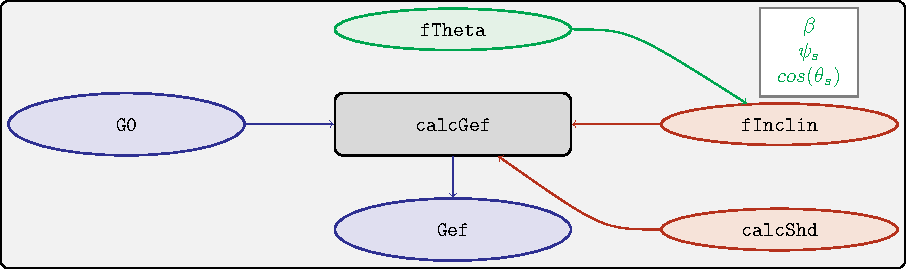
\includegraphics[keepaspectratio,width=\textwidth,height=0.5\textheight]{figuras/calcgef.pdf}
\caption{Cálculo de la radiación efectiva incidente en el plano del generador mediante la función \texttt{calcGef}, la cual emplea la función \texttt{fInclin} para el computo de las componentes efectivas, la función \texttt{fTheta} que provee a la función anterior los ángulos necesarios para su computo y la función \texttt{calcShd} que reprocesa el objeto de clase \texttt{Gef} resultante, añadiendole el efecto de las sombras producidas entres módulos. \label{fig:calcgef}}
\end{figure}
\begin{itemize}
\item \texttt{fTheta}: la cual, partiendo del ángulo de inclinación (\(\beta\)) y la orientación (\(\alpha\)), calcula el ángulo de inclinación en cada instante (\(\beta\)), el ángulo azimutal (\(\psi_s\)) y el coseno del ángulo de incidencia  de la radiación solar en la superficie (\(cos(\theta_s)\)).
Como principal argumento tiene \texttt{modeTrk}, el cual determina el sistema de seguimiento que tiene el sistema:
\begin{itemize}
\item \texttt{fixed}: para sistemas estáticos.
\end{itemize}
\begin{lstlisting}[numbers=left,language=r,label= ,caption= ,captionpos=b]
BTd <- fBTd(mode = 'prom')[6] 
sol <- calcSol(lat, BTd = BTd, keep.night = FALSE)
beta <- lat - 10
alfa <- 0
angGen_fixed <- fTheta(sol = sol, beta = beta, alfa = alfa,
                 modeTrk = 'fixed')
show(angGen_fixed)
\end{lstlisting}

\begin{verbatim}
		  Dates      Beta  Alfa   cosTheta
		 <POSc>     <num> <num>      <num>
 1: 2024-06-10 05:00:00 0.4747296     0 0.00000000
 2: 2024-06-10 06:00:00 0.4747296     0 0.06990810
 3: 2024-06-10 07:00:00 0.4747296     0 0.30432148
 4: 2024-06-10 08:00:00 0.4747296     0 0.52263672
 5: 2024-06-10 09:00:00 0.4747296     0 0.70998013
 6: 2024-06-10 10:00:00 0.4747296     0 0.85358815
 7: 2024-06-10 11:00:00 0.4747296     0 0.94367686
 8: 2024-06-10 12:00:00 0.4747296     0 0.97410861
 9: 2024-06-10 13:00:00 0.4747296     0 0.94281011
10: 2024-06-10 14:00:00 0.4747296     0 0.85191372
11: 2024-06-10 15:00:00 0.4747296     0 0.70761218
12: 2024-06-10 16:00:00 0.4747296     0 0.51973665
13: 2024-06-10 17:00:00 0.4747296     0 0.30108697
14: 2024-06-10 18:00:00 0.4747296     0 0.06655958
15: 2024-06-10 19:00:00 0.4747296     0 0.00000000
\end{verbatim}

\begin{itemize}
\item \texttt{two}: para sistemas de seguimiento de doble eje.
\end{itemize}
\begin{lstlisting}[numbers=left,language=r,label= ,caption= ,captionpos=b]
angGen_two <- fTheta(sol = sol, beta = beta, alfa = alfa,
                     modeTrk = 'two')
show(angGen_two)
\end{lstlisting}

\begin{verbatim}
		  Dates      Beta         Alfa cosTheta
		 <POSc>     <num>        <num>    <num>
 1: 2024-06-10 05:00:00 1.5220852 -2.043678875        1
 2: 2024-06-10 06:00:00 1.3300857 -1.896688029        1
 3: 2024-06-10 07:00:00 1.1285281 -1.756655282        1
 4: 2024-06-10 08:00:00 0.9215732 -1.612213267        1
 5: 2024-06-10 09:00:00 0.7134716 -1.445120762        1
 6: 2024-06-10 10:00:00 0.5110180 -1.215351693        1
 7: 2024-06-10 11:00:00 0.3328578 -0.809087856        1
 8: 2024-06-10 12:00:00 0.2466893  0.006963841        1
 9: 2024-06-10 13:00:00 0.3349967  0.817155564        1
10: 2024-06-10 14:00:00 0.5137803  1.219398208        1
11: 2024-06-10 15:00:00 0.7163931  1.447776194        1
12: 2024-06-10 16:00:00 0.9245147  1.614353339        1
13: 2024-06-10 17:00:00 1.1314208  1.758631827        1
14: 2024-06-10 18:00:00 1.3328735  1.898691776        1
15: 2024-06-10 19:00:00 1.5247042  2.045849315        1
\end{verbatim}

\begin{itemize}
\item \texttt{horiz}: para sistemas de seguimiento horizontal Norte-Sur.
\end{itemize}
\begin{lstlisting}[numbers=left,language=r,label= ,caption= ,captionpos=b]
angGen_horiz <- fTheta(sol = sol, beta = beta, alfa = alfa,
                       modeTrk = 'horiz')
show(angGen_horiz)
\end{lstlisting}

\begin{verbatim}
		  Dates        Beta      Alfa  cosTheta
		 <POSc>       <num>     <num>     <num>
 1: 2024-06-10 05:00:00 1.516091993 -1.570796 0.8905353
 2: 2024-06-10 06:00:00 1.317263961 -1.570796 0.9504350
 3: 2024-06-10 07:00:00 1.121771495 -1.570796 0.9859551
 4: 2024-06-10 08:00:00 0.921160041 -1.570796 0.9994560
 5: 2024-06-10 09:00:00 0.709555740 -1.570796 0.9966296
 6: 2024-06-10 10:00:00 0.483954771 -1.570796 0.9854098
 7: 2024-06-10 11:00:00 0.245151627 -1.570796 0.9742418
 8: 2024-06-10 12:00:00 0.001753607  1.570796 0.9697277
 9: 2024-06-10 13:00:00 0.248597042  1.570796 0.9743648
10: 2024-06-10 14:00:00 0.487239436  1.570796 0.9855868
11: 2024-06-10 15:00:00 0.712638107  1.570796 0.9967482
12: 2024-06-10 16:00:00 0.924058412  1.570796 0.9993956
13: 2024-06-10 17:00:00 1.124550569  1.570796 0.9856166
14: 2024-06-10 18:00:00 1.320024608  1.570796 0.9497600
15: 2024-06-10 19:00:00 1.518974473  1.570796 0.8895182
\end{verbatim}

También, tiene un argumento \texttt{BT} que indica cuando se usa la técnica de backtracking para un sistema horizontal Norte-Sur. Para funcionar, necesita de los argumentos \texttt{struct}, el cual presenta una lista con la altura de los módulos, y \texttt{dist}, el cual presenta un \texttt{data.frame} (o \texttt{data.table}) con la distancia que separa los módulos en la dirección Este-Oeste.
\begin{lstlisting}[numbers=left,language=r,label= ,caption= ,captionpos=b]
struct <- list(L = 1)
distances <- data.table(Lew = 2)
angGen_BT <- fTheta(sol = sol, beta = beta, alfa = alfa,
                    modeTrk = 'horiz', BT = TRUE,
                    struct = struct, dist = distances)
show(angGen_BT)
\end{lstlisting}

\begin{verbatim}
		  Dates        Beta      Alfa   cosTheta
		 <POSc>       <num>     <num>      <num>
 1: 2024-06-10 05:00:00 0.054868903 -1.570796 0.09738369
 2: 2024-06-10 06:00:00 0.271972628 -1.570796 0.47678565
 3: 2024-06-10 07:00:00 0.602487004 -1.570796 0.85598103
 4: 2024-06-10 08:00:00 0.921160041 -1.570796 0.99945597
 5: 2024-06-10 09:00:00 0.709555740 -1.570796 0.99662956
 6: 2024-06-10 10:00:00 0.483954771 -1.570796 0.98540983
 7: 2024-06-10 11:00:00 0.245151627 -1.570796 0.97424175
 8: 2024-06-10 12:00:00 0.001753607  1.570796 0.96972767
 9: 2024-06-10 13:00:00 0.248597042  1.570796 0.97436477
10: 2024-06-10 14:00:00 0.487239436  1.570796 0.98558683
11: 2024-06-10 15:00:00 0.712638107  1.570796 0.99674816
12: 2024-06-10 16:00:00 0.924058412  1.570796 0.99939563
13: 2024-06-10 17:00:00 0.595256963  1.570796 0.85074877
14: 2024-06-10 18:00:00 0.268563625  1.570796 0.47136897
15: 2024-06-10 19:00:00 0.051961679  1.570796 0.09215170
\end{verbatim}

\item \texttt{fInclin}: la cual, partiendo del resultado de \texttt{fTheta} y de un objeto de clase \texttt{G0}, cálcula la irradiancia solar incidente en una superficie inclinada junto con los efectos del ángulo de incidencia y la suciedad para obtener la irradiancia efectiva.
Como argumentos principales están:
\begin{itemize}
\item \texttt{iS}: permite seleccionar entre 4 valores del 1 al 4 correspondientes al grado de suciedad del módulo. Siendo 1 limpio y 4 alto y basandose en los valores de la tabla \ref{tab:coef-perd} calcula la irradiancia efectiva. Por defecto tiene valor 2 (grado de suciedad bajo).
\end{itemize}
\begin{lstlisting}[numbers=left,language=r,label= ,caption= ,captionpos=b]
compI <- calcG0(lat, dataRad = prom, keep.night = FALSE)
sol <- calcSol(lat, BTi = indexI(compI))
angGen <- fTheta(sol = sol, beta = beta, alfa = alfa)
inclin_limpio <- fInclin(compI = compI, angGen = angGen, iS = 1)
show(inclin_limpio)
\end{lstlisting}

\begin{verbatim}
		   Dates        Bo       Bn        G         D       Di        Dc         B         R
		  <POSc>     <num>    <num>    <num>     <num>    <num>     <num>     <num>     <num>
  1: 2024-01-17 08:00:00  514.5612 365.8727 186.4590  52.34286 25.82073  26.52212 133.18653 0.9295706
  2: 2024-01-17 09:00:00  792.6980 464.2106 366.6704 103.96230 52.12242  51.83988 260.32510 2.3830282
  3: 2024-01-17 10:00:00 1010.9063 541.3602 536.6247 145.69981 68.60264  77.09717 387.15997 3.7648749
  4: 2024-01-17 11:00:00 1154.3223 592.0663 662.0048 173.72247 77.44190  96.28057 483.49354 4.7887550
  5: 2024-01-17 12:00:00 1213.1770 612.8750 716.5974 185.35767 80.61172 104.74595 526.00427 5.2354830
 ---                                                                                                 
141: 2024-12-13 12:00:00 1181.1554 470.2512 578.4583 180.82966 95.85462  84.97504 393.39650 4.2321949
142: 2024-12-13 13:00:00 1129.5610 453.5904 536.8668 170.08970 91.70559  78.38411 362.88341 3.8937280
143: 2024-12-13 14:00:00  994.4636 409.9651 434.0673 142.25355 79.88147  62.37208 288.75488 3.0588416
144: 2024-12-13 15:00:00  785.0640 342.3463 292.1950  99.92831 58.81096  41.11735 190.35496 1.9117069
145: 2024-12-13 16:00:00  515.6229 255.3390 140.8937  46.94651 26.80445  20.14206  93.24874 0.6984426
	     FTb        FTd       FTr     Dief      Dcef      Gef       Def       Bef       Ref
	   <num>      <num>     <num>    <num>     <num>    <num>     <num>     <num>     <num>
  1: 0.115032290 0.05043622 0.2503398 24.51843  23.47122 166.5523  47.98966 117.86578 0.6968621
  2: 0.034235799 0.05043622 0.2503398 49.49356  50.06510 352.7578  99.55866 251.41266 1.7864615
  3: 0.012139104 0.05043622 0.2503398 65.14258  76.16128 526.5864 141.30386 382.46020 2.8223770
  4: 0.005426675 0.05043622 0.2503398 73.53602  95.75809 653.7538 169.29411 480.86978 3.5899392
  5: 0.003640433 0.05043622 0.2503398 76.54597 104.36463 708.9248 180.91060 524.08939 3.9248333
 ---                                                                                           
141: 0.004516349 0.05043622 0.2503398 91.02007  84.59127 570.4038 175.61134 391.61978 3.1727082
142: 0.006269898 0.05043622 0.2503398 87.08031  77.89265 528.5001 164.97296 360.60816 2.9189730
143: 0.013120704 0.05043622 0.2503398 75.85255  61.55372 424.6656 137.40626 284.96622 2.2930919
144: 0.035287438 0.05043622 0.2503398 55.84476  39.66642 280.5821  95.51118 183.63782 1.4331306
145: 0.114223038 0.05043622 0.2503398 25.45254  17.84137 126.4151  43.29391  82.59758 0.5235947
\end{verbatim}

\begin{lstlisting}[numbers=left,language=r,label= ,caption= ,captionpos=b]
inclin_sucio <- fInclin(compI = compI, angGen = angGen, iS = 4)
show(inclin_sucio)
\end{lstlisting}

\begin{verbatim}
		   Dates        Bo       Bn        G         D       Di        Dc         B         R
		  <POSc>     <num>    <num>    <num>     <num>    <num>     <num>     <num>     <num>
  1: 2024-01-17 08:00:00  514.5612 365.8727 186.4590  52.34286 25.82073  26.52212 133.18653 0.9295706
  2: 2024-01-17 09:00:00  792.6980 464.2106 366.6704 103.96230 52.12242  51.83988 260.32510 2.3830282
  3: 2024-01-17 10:00:00 1010.9063 541.3602 536.6247 145.69981 68.60264  77.09717 387.15997 3.7648749
  4: 2024-01-17 11:00:00 1154.3223 592.0663 662.0048 173.72247 77.44190  96.28057 483.49354 4.7887550
  5: 2024-01-17 12:00:00 1213.1770 612.8750 716.5974 185.35767 80.61172 104.74595 526.00427 5.2354830
 ---                                                                                                 
141: 2024-12-13 12:00:00 1181.1554 470.2512 578.4583 180.82966 95.85462  84.97504 393.39650 4.2321949
142: 2024-12-13 13:00:00 1129.5610 453.5904 536.8668 170.08970 91.70559  78.38411 362.88341 3.8937280
143: 2024-12-13 14:00:00  994.4636 409.9651 434.0673 142.25355 79.88147  62.37208 288.75488 3.0588416
144: 2024-12-13 15:00:00  785.0640 342.3463 292.1950  99.92831 58.81096  41.11735 190.35496 1.9117069
145: 2024-12-13 16:00:00  515.6229 255.3390 140.8937  46.94651 26.80445  20.14206  93.24874 0.6984426
	    FTb        FTd       FTr     Dief     Dcef      Gef       Def       Bef       Ref
	  <num>      <num>     <num>    <num>    <num>    <num>     <num>     <num>     <num>
  1: 0.24100175 0.09714708 0.3918962 21.44734 18.51982 133.4885  39.96716  93.00127 0.5200533
  2: 0.10321543 0.09714708 0.3918962 43.29416 42.77007 302.1765  86.06424 214.77909 1.3331982
  3: 0.04727214 0.09714708 0.3918962 56.98305 67.57641 466.0152 124.55946 339.34944 2.1062799
  4: 0.02455379 0.09714708 0.3918962 64.32515 86.40320 587.2996 150.72835 433.89218 2.6790952
  5: 0.01743586 0.09714708 0.3918962 66.95809 94.68605 640.0594 161.64413 475.48630 2.9290196
 ---                                                                                         
141: 0.02100686 0.09714708 0.3918962 79.61921 76.53478 512.8436 156.15400 354.32187 2.3677246
142: 0.02771140 0.09714708 0.3918962 76.17293 70.11502 473.0675 146.28795 324.60121 2.1783674
143: 0.05023795 0.09714708 0.3918962 66.35152 54.49955 374.8709 120.85106 252.30856 1.7112857
144: 0.10550059 0.09714708 0.3918962 48.84983 33.83709 240.4070  82.68692 156.65061 1.0695149
145: 0.23984890 0.09714708 0.3918962 22.26444 14.08613 101.9538  36.35057  65.21248 0.3907476
\end{verbatim}

\begin{itemize}
\item \texttt{alb} Correspondiente al coeficiente de reflexión del terreno para la irradiancia de albedo. Por defecto tiene un valor de 0,2 (valor aceptable para un terreno normal).
\end{itemize}
\begin{lstlisting}[numbers=left,language=r,label= ,caption= ,captionpos=b]
inclin_alb0 <- fInclin(compI = compI, angGen = angGen, alb = 0)
show(inclin_alb0)
\end{lstlisting}

\begin{verbatim}
		   Dates        Bo       Bn        G         D       Di        Dc         B     R
		  <POSc>     <num>    <num>    <num>     <num>    <num>     <num>     <num> <num>
  1: 2024-01-17 08:00:00  514.5612 365.8727 185.5294  52.34286 25.82073  26.52212 133.18653     0
  2: 2024-01-17 09:00:00  792.6980 464.2106 364.2874 103.96230 52.12242  51.83988 260.32510     0
  3: 2024-01-17 10:00:00 1010.9063 541.3602 532.8598 145.69981 68.60264  77.09717 387.15997     0
  4: 2024-01-17 11:00:00 1154.3223 592.0663 657.2160 173.72247 77.44190  96.28057 483.49354     0
  5: 2024-01-17 12:00:00 1213.1770 612.8750 711.3619 185.35767 80.61172 104.74595 526.00427     0
 ---                                                                                             
141: 2024-12-13 12:00:00 1181.1554 470.2512 574.2262 180.82966 95.85462  84.97504 393.39650     0
142: 2024-12-13 13:00:00 1129.5610 453.5904 532.9731 170.08970 91.70559  78.38411 362.88341     0
143: 2024-12-13 14:00:00  994.4636 409.9651 431.0084 142.25355 79.88147  62.37208 288.75488     0
144: 2024-12-13 15:00:00  785.0640 342.3463 290.2833  99.92831 58.81096  41.11735 190.35496     0
145: 2024-12-13 16:00:00  515.6229 255.3390 140.1953  46.94651 26.80445  20.14206  93.24874     0
	     FTb        FTd       FTr     Dief      Dcef      Gef       Def       Bef   Ref
	   <num>      <num>     <num>    <num>     <num>    <num>     <num>     <num> <num>
  1: 0.156321477 0.06473603 0.2994808 23.66622  21.92862 155.7141  45.59484 110.11928     0
  2: 0.054197292 0.06473603 0.2994808 47.77325  48.04970 337.1148  95.82295 241.29186     0
  3: 0.021399057 0.06473603 0.2994808 62.87835  73.93841 508.1144 136.81676 371.29761     0
  4: 0.010185772 0.06473603 0.2994808 70.98005  93.39388 633.3713 164.37393 468.99741     0
  5: 0.006996517 0.06473603 0.2994808 73.88537 101.93283 687.6958 175.81821 511.87759     0
 ---                                                                                       
141: 0.008575046 0.06473603 0.2994808 87.85638  82.56145 552.6405 170.41783 382.22264     0
142: 0.011653979 0.06473603 0.2994808 84.05356  75.92121 511.4560 159.97477 351.48128     0
143: 0.022965930 0.06473603 0.2994808 73.21605  59.72086 409.4178 132.93691 276.48089     0
144: 0.055666181 0.06473603 0.2994808 53.90370  38.05193 268.1191  91.95563 176.16345     0
145: 0.155368802 0.06473603 0.2994808 24.56786  16.67236 118.4258  41.24021  77.18558     0
\end{verbatim}

\begin{lstlisting}[numbers=left,language=r,label= ,caption= ,captionpos=b]
inclin_alb1 <- fInclin(compI = compI, angGen = angGen, alb = 1)
show(inclin_alb1)
\end{lstlisting}

\begin{verbatim}
		   Dates        Bo       Bn        G         D       Di        Dc         B         R
		  <POSc>     <num>    <num>    <num>     <num>    <num>     <num>     <num>     <num>
  1: 2024-01-17 08:00:00  514.5612 365.8727 190.1772  52.34286 25.82073  26.52212 133.18653  4.647853
  2: 2024-01-17 09:00:00  792.6980 464.2106 376.2025 103.96230 52.12242  51.83988 260.32510 11.915141
  3: 2024-01-17 10:00:00 1010.9063 541.3602 551.6842 145.69981 68.60264  77.09717 387.15997 18.824375
  4: 2024-01-17 11:00:00 1154.3223 592.0663 681.1598 173.72247 77.44190  96.28057 483.49354 23.943775
  5: 2024-01-17 12:00:00 1213.1770 612.8750 737.5394 185.35767 80.61172 104.74595 526.00427 26.177415
 ---                                                                                                 
141: 2024-12-13 12:00:00 1181.1554 470.2512 595.3871 180.82966 95.85462  84.97504 393.39650 21.160975
142: 2024-12-13 13:00:00 1129.5610 453.5904 552.4417 170.08970 91.70559  78.38411 362.88341 19.468640
143: 2024-12-13 14:00:00  994.4636 409.9651 446.3026 142.25355 79.88147  62.37208 288.75488 15.294208
144: 2024-12-13 15:00:00  785.0640 342.3463 299.8418  99.92831 58.81096  41.11735 190.35496  9.558535
145: 2024-12-13 16:00:00  515.6229 255.3390 143.6875  46.94651 26.80445  20.14206  93.24874  3.492213
	     FTb        FTd       FTr     Dief      Dcef      Gef       Def       Bef       Ref
	   <num>      <num>     <num>    <num>     <num>    <num>     <num>     <num>     <num>
  1: 0.156321477 0.06473603 0.2994808 23.66622  21.92862 158.9049  45.59484 110.11928  3.190792
  2: 0.054197292 0.06473603 0.2994808 47.77325  48.04970 345.2947  95.82295 241.29186  8.179849
  3: 0.021399057 0.06473603 0.2994808 62.87835  73.93841 521.0375 136.81676 371.29761 12.923098
  4: 0.010185772 0.06473603 0.2994808 70.98005  93.39388 649.8089 164.37393 468.99741 16.437612
  5: 0.006996517 0.06473603 0.2994808 73.88537 101.93283 705.6668 175.81821 511.87759 17.971025
 ---                                                                                           
141: 0.008575046 0.06473603 0.2994808 87.85638  82.56145 567.1677 170.41783 382.22264 14.527195
142: 0.011653979 0.06473603 0.2994808 84.05356  75.92121 524.8214 159.97477 351.48128 13.365392
143: 0.022965930 0.06473603 0.2994808 73.21605  59.72086 419.9174 132.93691 276.48089 10.499608
144: 0.055666181 0.06473603 0.2994808 53.90370  38.05193 274.6811  91.95563 176.16345  6.562018
145: 0.155368802 0.06473603 0.2994808 24.56786  16.67236 120.8232  41.24021  77.18558  2.397435
\end{verbatim}

Además, cuenta con dos argumentos adicionales, \texttt{horizBright}, el cual, cuando su valor es \texttt{TRUE} (el que tiene por defecto), realiza una corrección de la radiación difusa \cite{REINDL19909}, y \texttt{HCPV}, es el acrónimo de \textbf{High Concentration PV system}\footnote{la tencología de concentración fotovoltaica funciona gracias a unos dispositivos ópticos que permiten concentrar la radiación solar sobre una célula fotovoltaica de tamaño reducido pero con una eficiencia muy superior alas células tradicionales. Con ello se consigue emplear menor cantidad de semiconductores reduciendo los costes.} (sistema fotovoltaico de alta concentración) que cuando su valor es \texttt{TRUE} (por defecto está puesto en \texttt{FALSE}), anula los valores de radiación difusa y de albedo.
\begin{lstlisting}[numbers=left,language=r,label= ,caption= ,captionpos=b]
inclin_horizBright <- fInclin(compI = compI, angGen = angGen,
                              horizBright = FALSE)
show(inclin_horizBright)
\end{lstlisting}

\begin{verbatim}
		   Dates        Bo       Bn        G         D       Di        Dc         B         R
		  <POSc>     <num>    <num>    <num>     <num>    <num>     <num>     <num>     <num>
  1: 2024-01-17 08:00:00  514.5612 365.8727 186.2091  52.09303 25.57090  26.52212 133.18653 0.9295706
  2: 2024-01-17 09:00:00  792.6980 464.2106 366.1413 103.43314 51.59325  51.83988 260.32510 2.3830282
  3: 2024-01-17 10:00:00 1010.9063 541.3602 535.9087 144.98390 67.88673  77.09717 387.15997 3.7648749
  4: 2024-01-17 11:00:00 1154.3223 592.0663 661.1846 172.90227 76.62170  96.28057 483.49354 4.7887550
  5: 2024-01-17 12:00:00 1213.1770 612.8750 715.7390 184.49921 79.75326 104.74595 526.00427 5.2354830
 ---                                                                                                 
141: 2024-12-13 12:00:00 1181.1554 470.2512 577.4973 179.86860 94.89356  84.97504 393.39650 4.2321949
142: 2024-12-13 13:00:00 1129.5610 453.5904 535.9539 169.17679 90.79268  78.38411 362.88341 3.8937280
143: 2024-12-13 14:00:00  994.4636 409.9651 433.2885 141.47476 79.10268  62.37208 288.75488 3.0588416
144: 2024-12-13 15:00:00  785.0640 342.3463 291.6442  99.37758 58.26023  41.11735 190.35496 1.9117069
145: 2024-12-13 16:00:00  515.6229 255.3390 140.6606  46.71344 26.57138  20.14206  93.24874 0.6984426
	     FTb        FTd       FTr     Dief      Dcef      Gef       Def       Bef       Ref
	   <num>      <num>     <num>    <num>     <num>    <num>     <num>     <num>     <num>
  1: 0.156321477 0.06473603 0.2994808 23.43723  21.92862 156.1233  45.36586 110.11928 0.6381583
  2: 0.054197292 0.06473603 0.2994808 47.28824  48.04970 338.2658  95.33794 241.29186 1.6359698
  3: 0.021399057 0.06473603 0.2994808 62.22217  73.93841 510.0428 136.16059 371.29761 2.5846197
  4: 0.010185772 0.06473603 0.2994808 70.22829  93.39388 635.9071 163.62217 468.99741 3.2875223
  5: 0.006996517 0.06473603 0.2994808 73.09855 101.93283 690.5032 175.03138 511.87759 3.5942050
 ---                                                                                           
141: 0.008575046 0.06473603 0.2994808 86.97552  82.56145 554.6650 169.53697 382.22264 2.9054390
142: 0.011653979 0.06473603 0.2994808 83.21682  75.92121 513.2924 159.13803 351.48128 2.6730784
143: 0.022965930 0.06473603 0.2994808 72.50225  59.72086 410.8039 132.22311 276.48089 2.0999216
144: 0.055666181 0.06473603 0.2994808 53.39892  38.05193 268.9267  91.45086 176.16345 1.3124036
145: 0.155368802 0.06473603 0.2994808 24.35423  16.67236 118.6917  41.02659  77.18558 0.4794870
\end{verbatim}

\begin{lstlisting}[numbers=left,language=r,label= ,caption= ,captionpos=b]
inclin_HCPV <- fInclin(compI = compI, angGen = angGen,
                       HCPV = TRUE)
show(inclin_HCPV)
\end{lstlisting}

\begin{verbatim}
		   Dates        Bo       Bn        G         D       Di        Dc         B         R
		  <POSc>     <num>    <num>    <num>     <num>    <num>     <num>     <num>     <num>
  1: 2024-01-17 08:00:00  514.5612 365.8727 186.4590  52.34286 25.82073  26.52212 133.18653 0.9295706
  2: 2024-01-17 09:00:00  792.6980 464.2106 366.6704 103.96230 52.12242  51.83988 260.32510 2.3830282
  3: 2024-01-17 10:00:00 1010.9063 541.3602 536.6247 145.69981 68.60264  77.09717 387.15997 3.7648749
  4: 2024-01-17 11:00:00 1154.3223 592.0663 662.0048 173.72247 77.44190  96.28057 483.49354 4.7887550
  5: 2024-01-17 12:00:00 1213.1770 612.8750 716.5974 185.35767 80.61172 104.74595 526.00427 5.2354830
 ---                                                                                                 
141: 2024-12-13 12:00:00 1181.1554 470.2512 578.4583 180.82966 95.85462  84.97504 393.39650 4.2321949
142: 2024-12-13 13:00:00 1129.5610 453.5904 536.8668 170.08970 91.70559  78.38411 362.88341 3.8937280
143: 2024-12-13 14:00:00  994.4636 409.9651 434.0673 142.25355 79.88147  62.37208 288.75488 3.0588416
144: 2024-12-13 15:00:00  785.0640 342.3463 292.1950  99.92831 58.81096  41.11735 190.35496 1.9117069
145: 2024-12-13 16:00:00  515.6229 255.3390 140.8937  46.94651 26.80445  20.14206  93.24874 0.6984426
	     FTb        FTd       FTr  Dief  Dcef       Gef   Def       Bef   Ref
	   <num>      <num>     <num> <num> <num>     <num> <num>     <num> <num>
  1: 0.156321477 0.06473603 0.2994808     0     0 110.11928     0 110.11928     0
  2: 0.054197292 0.06473603 0.2994808     0     0 241.29186     0 241.29186     0
  3: 0.021399057 0.06473603 0.2994808     0     0 371.29761     0 371.29761     0
  4: 0.010185772 0.06473603 0.2994808     0     0 468.99741     0 468.99741     0
  5: 0.006996517 0.06473603 0.2994808     0     0 511.87759     0 511.87759     0
 ---                                                                             
141: 0.008575046 0.06473603 0.2994808     0     0 382.22264     0 382.22264     0
142: 0.011653979 0.06473603 0.2994808     0     0 351.48128     0 351.48128     0
143: 0.022965930 0.06473603 0.2994808     0     0 276.48089     0 276.48089     0
144: 0.055666181 0.06473603 0.2994808     0     0 176.16345     0 176.16345     0
145: 0.155368802 0.06473603 0.2994808     0     0  77.18558     0  77.18558     0
\end{verbatim}
\end{itemize}

Finalmente, esta función le otorga estos datos a la función \texttt{calcGef} para que produzca un objeto de clase \texttt{Gef} como resultado. Esta función tiene como argumentos principales los mismos que los que tiene \texttt{calcG0} \ref{sec:radiacion-plano-horizontal}, es decir, \texttt{modeRad} y \texttt{dataRad}. Y además, como es lógico, con todos los argumentos mencionados con anterioridad en \texttt{fTheta} y \texttt{fInclin}.
\begin{lstlisting}[numbers=left,language=r,label= ,caption= ,captionpos=b]
gef_prom <- calcGef(lat = lat, modeTrk = 'two', modeRad = 'prom',
                    dataRad = prom,
                    beta = lat-10, alfa = 0,
                    iS = 2, alb = 0.2,
                    horizBright = TRUE, HCPV = FALSE)
show(gef_prom)
\end{lstlisting}

\begin{verbatim}
Object of class  Gef 

Source of meteorological information: prom- 

Latitude of source:  37.2 degrees
Latitude for calculations:  37.2 degrees

Monthly avarages:
        Dates      Bod       Bnd        Gd       Dd       Bd      Gefd     Defd     Befd
       <char>    <num>     <num>     <num>    <num>    <num>     <num>    <num>    <num>
 1: Jan. 2024 14.13536  4.924221  6.522313 1.440413 4.924221  6.348801 1.384087 4.825736
 2: Feb. 2024 15.42754  5.034287  6.875052 1.672079 5.034287  6.680139 1.599929 4.933601
 3: Mar. 2024 16.58107  5.163713  7.329138 1.998110 5.163713  7.104641 1.902356 5.060439
 4: Apr. 2024 17.64047  6.408617  8.843422 2.265896 6.408617  8.578222 2.158071 6.280444
 5: May. 2024 18.70771  7.617499 10.178196 2.394606 7.617499  9.885240 2.284334 7.465149
 6: Jun. 2024 19.87238  9.102430 11.606533 2.329653 9.102430 11.293417 2.230338 8.920381
 7: Jul. 2024 18.51695 10.037233 11.801533 2.029150 9.589205 11.495648 1.948530 9.397421
 8: Aug. 2024 17.34098  8.640959 10.777404 1.947410 8.640959 10.493150 1.869393 8.468140
 9: Sep. 2024 16.25295  6.698488  8.831006 1.948075 6.698488  8.584604 1.864962 6.564518
10: Oct. 2024 15.16994  4.546024  6.418653 1.711039 4.546024  6.226290 1.631551 4.455104
11: Nov. 2024 14.00493  4.638289  6.247341 1.452953 4.638289  6.076159 1.393353 4.545523
12: Dec. 2024 12.70717  3.439788  4.825181 1.254616 3.439788  4.685547 1.198824 3.370992

Yearly values:
   Dates      Bod      Bnd       Gd       Dd       Bd     Gefd    Defd     Befd
   <int>    <num>    <num>    <num>    <num>    <num>    <num>   <num>    <num>
1:  2024 5988.455 2326.882 3058.651 684.4232 2312.993 2973.115 654.591 2266.733
-----------------
Mode of tracking:  two 
    Inclination limit: 90
\end{verbatim}

Sin embargo, como argumento importante está \texttt{modeShd}, el cual permite incluir el efecto de las sombras entre módulos al objeto \texttt{Gef} mediante el uso de la función \texttt{calcShd}. Esta opción añade las variables \texttt{Gef0}, \texttt{Def0} y \texttt{Bef0} las cuales son las componentes de radiación efectiva previas a aplicar el efecto de las sombras con el fin de poder comparar.
\begin{lstlisting}[numbers=left,language=r,label= ,caption= ,captionpos=b]
struct <- list(W=23.11, L=9.8, Nrow=2, Ncol=8)
distances <- data.table(Lew=40, Lns=30, H=0)
gef_shd <- calcShd(radEf = gef_prom, modeShd = 'prom',
                   struct = struct, distances = distances)
show(gef_shd)
\end{lstlisting}

\begin{verbatim}
Object of class  Gef 

Source of meteorological information: prom- 

Latitude of source:  37.2 degrees
Latitude for calculations:  37.2 degrees

Monthly avarages:
        Dates     Gef0d    Def0d    Bef0d        Gd       Dd       Bd      Gefd     Defd     Befd
       <char>     <num>    <num>    <num>     <num>    <num>    <num>     <num>    <num>    <num>
 1: Jan. 2024  6.348801 1.384087 4.825736  6.522313 1.440413 4.924221  6.104126 1.343455 4.621693
 2: Feb. 2024  6.680139 1.599929 4.933601  6.875052 1.672079 5.034287  6.406274 1.553670 4.705996
 3: Mar. 2024  7.104641 1.902356 5.060439  7.329138 1.998110 5.163713  6.788630 1.848127 4.798657
 4: Apr. 2024  8.578222 2.158071 6.280444  8.843422 2.265896 6.408617  8.295340 2.112064 6.043569
 5: May. 2024  9.885240 2.284334 7.465149 10.178196 2.394606 7.617499  9.688308 2.253942 7.298609
 6: Jun. 2024 11.293417 2.230338 8.920381 11.606533 2.329653 9.102430 11.115054 2.205314 8.767042
 7: Jul. 2024 11.495648 1.948530 9.397421 11.801533 2.029150 9.589205 11.308971 1.924962 9.234312
 8: Aug. 2024 10.493150 1.869393 8.468140 10.777404 1.947410 8.640959 10.196758 1.830334 8.210807
 9: Sep. 2024  8.584604 1.864962 6.564518  8.831006 1.948075 6.698488  8.228309 1.810198 6.262986
10: Oct. 2024  6.226290 1.631551 4.455104  6.418653 1.711039 4.546024  6.018374 1.595528 4.283212
11: Nov. 2024  6.076159 1.393353 4.545523  6.247341 1.452953 4.638289  5.875732 1.359514 4.378935
12: Dec. 2024  4.685547 1.198824 3.370992  4.825181 1.254616 3.439788  4.575893 1.179346 3.280817

Yearly values:
   Dates    Gef0d   Def0d    Bef0d       Gd       Dd       Bd     Gefd     Defd     Befd
   <int>    <num>   <num>    <num>    <num>    <num>    <num>    <num>    <num>    <num>
1:  2024 2973.115 654.591 2266.733 3058.651 684.4232 2312.993 2886.328 640.9157 2193.621
-----------------
Mode of tracking:  two 
    Inclination limit: 90
\end{verbatim}

\begin{lstlisting}[numbers=left,language=r,label= ,caption= ,captionpos=b]
gef_shd2 <- calcGef(lat = lat, modeTrk = 'two', dataRad = prom,
                    modeShd = 'prom', struct = struct, distances = distances)
show(gef_shd2)
\end{lstlisting}

\begin{verbatim}
Object of class  Gef 

Source of meteorological information: prom- 

Latitude of source:  37.2 degrees
Latitude for calculations:  37.2 degrees

Monthly avarages:
        Dates     Gef0d    Def0d    Bef0d        Gd       Dd       Bd      Gefd     Defd     Befd
       <char>     <num>    <num>    <num>     <num>    <num>    <num>     <num>    <num>    <num>
 1: Jan. 2024  6.348801 1.384087 4.825736  6.522313 1.440413 4.924221  6.104126 1.343455 4.621693
 2: Feb. 2024  6.680139 1.599929 4.933601  6.875052 1.672079 5.034287  6.406274 1.553670 4.705996
 3: Mar. 2024  7.104641 1.902356 5.060439  7.329138 1.998110 5.163713  6.788630 1.848127 4.798657
 4: Apr. 2024  8.578222 2.158071 6.280444  8.843422 2.265896 6.408617  8.295340 2.112064 6.043569
 5: May. 2024  9.885240 2.284334 7.465149 10.178196 2.394606 7.617499  9.688308 2.253942 7.298609
 6: Jun. 2024 11.293417 2.230338 8.920381 11.606533 2.329653 9.102430 11.115054 2.205314 8.767042
 7: Jul. 2024 11.495648 1.948530 9.397421 11.801533 2.029150 9.589205 11.308971 1.924962 9.234312
 8: Aug. 2024 10.493150 1.869393 8.468140 10.777404 1.947410 8.640959 10.196758 1.830334 8.210807
 9: Sep. 2024  8.584604 1.864962 6.564518  8.831006 1.948075 6.698488  8.228309 1.810198 6.262986
10: Oct. 2024  6.226290 1.631551 4.455104  6.418653 1.711039 4.546024  6.018374 1.595528 4.283212
11: Nov. 2024  6.076159 1.393353 4.545523  6.247341 1.452953 4.638289  5.875732 1.359514 4.378935
12: Dec. 2024  4.685547 1.198824 3.370992  4.825181 1.254616 3.439788  4.575893 1.179346 3.280817

Yearly values:
   Dates    Gef0d   Def0d    Bef0d       Gd       Dd       Bd     Gefd     Defd     Befd
   <int>    <num>   <num>    <num>    <num>    <num>    <num>    <num>    <num>    <num>
1:  2024 2973.115 654.591 2266.733 3058.651 684.4232 2312.993 2886.328 640.9157 2193.621
-----------------
Mode of tracking:  two 
    Inclination limit: 90
\end{verbatim}

El argumento \texttt{modeShd} puede ser de distintas maneras:
\begin{itemize}
\item \texttt{area}: el efecto de las sombras se calcula como una reducción proporcional de las irradiancias difusa circunsolar y directa.
\end{itemize}
\begin{lstlisting}[numbers=left,language=r,label= ,caption= ,captionpos=b]
gef_shdarea <- calcGef(lat, modeTrk = 'two', dataRad = prom,
                       modeShd = 'area',
                       struct = struct, distances = distances)
show(gef_shdarea)
\end{lstlisting}

\begin{verbatim}
Object of class  Gef 

Source of meteorological information: prom- 

Latitude of source:  37.2 degrees
Latitude for calculations:  37.2 degrees

Monthly avarages:
        Dates     Gef0d    Def0d    Bef0d        Gd       Dd       Bd      Gefd     Defd     Befd
       <char>     <num>    <num>    <num>     <num>    <num>    <num>     <num>    <num>    <num>
 1: Jan. 2024  6.348801 1.384087 4.825736  6.522313 1.440413 4.924221  5.877879 1.305883 4.433019
 2: Feb. 2024  6.680139 1.599929 4.933601  6.875052 1.672079 5.034287  6.291348 1.534257 4.610483
 3: Mar. 2024  7.104641 1.902356 5.060439  7.329138 1.998110 5.163713  6.743478 1.840379 4.761253
 4: Apr. 2024  8.578222 2.158071 6.280444  8.843422 2.265896 6.408617  8.254928 2.105491 6.009730
 5: May. 2024  9.885240 2.284334 7.465149 10.178196 2.394606 7.617499  9.660175 2.249601 7.274817
 6: Jun. 2024 11.293417 2.230338 8.920381 11.606533 2.329653 9.102430 11.089573 2.201739 8.745137
 7: Jul. 2024 11.495648 1.948530 9.397421 11.801533 2.029150 9.589205 11.282303 1.921596 9.211011
 8: Aug. 2024 10.493150 1.869393 8.468140 10.777404 1.947410 8.640959 10.154416 1.824754 8.174045
 9: Sep. 2024  8.584604 1.864962 6.564518  8.831006 1.948075 6.698488  8.177410 1.802375 6.219910
10: Oct. 2024  6.226290 1.631551 4.455104  6.418653 1.711039 4.546024  5.950189 1.583714 4.226840
11: Nov. 2024  6.076159 1.393353 4.545523  6.247341 1.452953 4.638289  5.705306 1.330740 4.237284
12: Dec. 2024  4.685547 1.198824 3.370992  4.825181 1.254616 3.439788  4.440179 1.155239 3.169210

Yearly values:
   Dates    Gef0d   Def0d    Bef0d       Gd       Dd       Bd     Gefd     Defd     Befd
   <int>    <num>   <num>    <num>    <num>    <num>    <num>    <num>    <num>    <num>
1:  2024 2973.115 654.591 2266.733 3058.651 684.4232 2312.993 2856.633 636.0199 2168.822
-----------------
Mode of tracking:  two 
    Inclination limit: 90
\end{verbatim}

\begin{itemize}
\item \texttt{prom}: cuando \texttt{modeTrk} es \texttt{two}, se puede calcular el efecto de las sombras de un seguidor promedio.
\end{itemize}
\begin{lstlisting}[numbers=left,language=r,label= ,caption= ,captionpos=b]
gef_shdprom <- calcGef(lat, modeTrk = 'two', dataRad = prom,
                       modeShd = c('area', 'prom'),
                       struct = struct, distances = distances)
show(gef_shdprom)
\end{lstlisting}

\begin{verbatim}
Object of class  Gef 

Source of meteorological information: prom- 

Latitude of source:  37.2 degrees
Latitude for calculations:  37.2 degrees

Monthly avarages:
        Dates     Gef0d    Def0d    Bef0d        Gd       Dd       Bd      Gefd     Defd     Befd
       <char>     <num>    <num>    <num>     <num>    <num>    <num>     <num>    <num>    <num>
 1: Jan. 2024  6.348801 1.384087 4.825736  6.522313 1.440413 4.924221  6.104126 1.343455 4.621693
 2: Feb. 2024  6.680139 1.599929 4.933601  6.875052 1.672079 5.034287  6.406274 1.553670 4.705996
 3: Mar. 2024  7.104641 1.902356 5.060439  7.329138 1.998110 5.163713  6.788630 1.848127 4.798657
 4: Apr. 2024  8.578222 2.158071 6.280444  8.843422 2.265896 6.408617  8.295340 2.112064 6.043569
 5: May. 2024  9.885240 2.284334 7.465149 10.178196 2.394606 7.617499  9.688308 2.253942 7.298609
 6: Jun. 2024 11.293417 2.230338 8.920381 11.606533 2.329653 9.102430 11.115054 2.205314 8.767042
 7: Jul. 2024 11.495648 1.948530 9.397421 11.801533 2.029150 9.589205 11.308971 1.924962 9.234312
 8: Aug. 2024 10.493150 1.869393 8.468140 10.777404 1.947410 8.640959 10.196758 1.830334 8.210807
 9: Sep. 2024  8.584604 1.864962 6.564518  8.831006 1.948075 6.698488  8.228309 1.810198 6.262986
10: Oct. 2024  6.226290 1.631551 4.455104  6.418653 1.711039 4.546024  6.018374 1.595528 4.283212
11: Nov. 2024  6.076159 1.393353 4.545523  6.247341 1.452953 4.638289  5.875732 1.359514 4.378935
12: Dec. 2024  4.685547 1.198824 3.370992  4.825181 1.254616 3.439788  4.575893 1.179346 3.280817

Yearly values:
   Dates    Gef0d   Def0d    Bef0d       Gd       Dd       Bd     Gefd     Defd     Befd
   <int>    <num>   <num>    <num>    <num>    <num>    <num>    <num>    <num>    <num>
1:  2024 2973.115 654.591 2266.733 3058.651 684.4232 2312.993 2886.328 640.9157 2193.621
-----------------
Mode of tracking:  two 
    Inclination limit: 90
\end{verbatim}

\begin{itemize}
\item \texttt{bt}: cuando \texttt{modeTrk} es \texttt{horiz}, se puede calcular el efecto del \emph{backtracking} en las sombras.
\end{itemize}
\begin{lstlisting}[numbers=left,language=r,label= ,caption= ,captionpos=b]
gef_shdhoriz <- calcGef(lat, modeTrk = 'horiz', dataRad = prom,
                        modeShd = 'area',
                        struct = struct, distances = distances)
show(gef_shdhoriz)
\end{lstlisting}

\begin{verbatim}
Object of class  Gef 

Source of meteorological information: prom- 

Latitude of source:  37.2 degrees
Latitude for calculations:  37.2 degrees

Monthly avarages:
        Dates     Gef0d     Def0d    Bef0d        Gd       Dd       Bd      Gefd      Defd     Befd
       <char>     <num>     <num>    <num>     <num>    <num>    <num>     <num>     <num>    <num>
 1: Jan. 2024  4.274445 1.0909303 3.118987  4.528022 1.166334 3.285391  3.826940 1.0166151 2.745797
 2: Feb. 2024  5.173537 1.3974587 3.699745  5.414413 1.484046 3.839622  4.709780 1.3191237 3.314324
 3: Mar. 2024  6.270377 1.8008592 4.379272  6.512568 1.906181 4.498391  5.856407 1.7298195 4.036342
 4: Apr. 2024  8.160354 2.1103041 5.938446  8.429640 2.222836 6.072611  7.744288 2.0426359 5.590049
 5: May. 2024  9.639011 2.2544315 7.260788  9.932830 2.366831 7.416258  9.158384 2.1802588 6.854334
 6: Jun. 2024 11.005388 2.1942042 8.675874 11.320680 2.294944 8.861907 10.355140 2.1029750 8.116855
 7: Jul. 2024 11.220872 1.9183453 9.163290 11.527430 2.000253 9.358648 10.747413 1.8585724 8.749603
 8: Aug. 2024 10.066277 1.8239013 8.112148 10.352216 1.904515 8.290847  9.601132 1.7626031 7.708301
 9: Sep. 2024  7.732062 1.7621525 5.864625  7.991813 1.852070 6.013507  7.317424 1.6984219 5.513717
10: Oct. 2024  5.023316 1.4757157 3.471271  5.250215 1.568278 3.591050  4.691499 1.4182254 3.196944
11: Nov. 2024  4.211801 1.1318865 3.014748  4.452659 1.209397 3.166130  3.846165 1.0701542 2.710845
12: Dec. 2024  3.024846 0.9640813 2.008270  3.237139 1.039367 2.135901  2.849995 0.9330218 1.864479

Yearly values:
   Dates    Gef0d    Def0d    Bef0d       Gd       Dd       Bd     Gefd     Defd     Befd
   <int>    <num>    <num>    <num>    <num>    <num>    <num>    <num>    <num>    <num>
1:  2024 2618.414 607.6589 1975.038 2714.415 640.9193 2030.645 2463.159 583.5528 1843.889
-----------------
Mode of tracking:  horiz 
    Inclination limit: 90
\end{verbatim}

\begin{lstlisting}[numbers=left,language=r,label= ,caption= ,captionpos=b]
gef_shdbt <- calcGef(lat, modeTrk = 'horiz', dataRad = prom,
                        modeShd = c('area', 'bt'),
                        struct = struct, distances = distances)
show(gef_shdbt)
\end{lstlisting}

\begin{verbatim}
Object of class  Gef 

Source of meteorological information: prom- 

Latitude of source:  37.2 degrees
Latitude for calculations:  37.2 degrees

Monthly avarages:
        Dates       Bod       Bnd        Gd       Dd       Bd      Gefd      Defd     Befd
       <char>     <num>     <num>     <num>    <num>    <num>     <num>     <num>    <num>
 1: Jan. 2024  8.071623  4.924221  4.069604 1.101792 2.902196  3.802336 1.0232875 2.724604
 2: Feb. 2024 10.170791  5.034287  4.943127 1.417056 3.445443  4.680459 1.3258434 3.287780
 3: Mar. 2024 12.816149  5.163713  6.094523 1.850253 4.148386  5.841685 1.7419635 4.020914
 4: Apr. 2024 15.326568  6.408617  8.007438 2.166491 5.716983  7.711198 2.0485357 5.560571
 5: May. 2024 16.624320  7.617499  9.439815 2.303156 7.000336  9.132906 2.1878882 6.833933
 6: Jun. 2024 17.408383  9.102430 10.652929 2.206022 8.288629 10.286974 2.0977541 8.059004
 7: Jul. 2024 16.861601 10.037233 11.038213 1.944739 8.935057 10.701158 1.8585291 8.712900
 8: Aug. 2024 15.551202  8.640959  9.872463 1.850828 7.878525  9.562356 1.7662720 7.678732
 9: Sep. 2024 13.422796  6.698488  7.568105 1.795358 5.655421  7.285297 1.7012821 5.487114
10: Oct. 2024 10.764846  4.546024  4.915408 1.521915 3.310678  4.666904 1.4246602 3.173452
11: Nov. 2024  8.434950  4.638289  4.079866 1.156410 2.854293  3.813241 1.0737415 2.681776
12: Dec. 2024  7.370928  3.439788  3.062505 1.023011 1.987550  2.836653 0.9441838 1.849321

Yearly values:
   Dates      Bod      Bnd       Gd       Dd       Bd     Gefd     Defd     Befd
   <int>    <num>    <num>    <num>    <num>    <num>    <num>    <num>    <num>
1:  2024 4662.615 2326.882 2555.869 620.2896 1896.422 2451.499 585.4392 1833.809
-----------------
Mode of tracking:  horiz 
    Inclination limit: 90
\end{verbatim}

\section{Producción eléctrica de un SFCR}
\label{sec:orga64d941}
\label{produccion-electrica-sfcr}
Con la radiación efectiva, se puede estimar la producción eléctrica que va a tener un sistema fotovoltaico conectado a red. Esta estimación, se puede calcular mediante la función \texttt{prodGCPV} [\ref{subsec:prodgcpv}] la cual mediante la función \texttt{fProd} [\ref{subsec:fprod}] procesa un objeto de clase \texttt{Gef} y obtiene un objeto \texttt{ProdGCPV}.

Como se puede ver en la figura \ref{fig:prodgcpv}, \texttt{prodGCPV} funciona gracias a la siguiente función:
\begin{figure}[htbp]
\centering
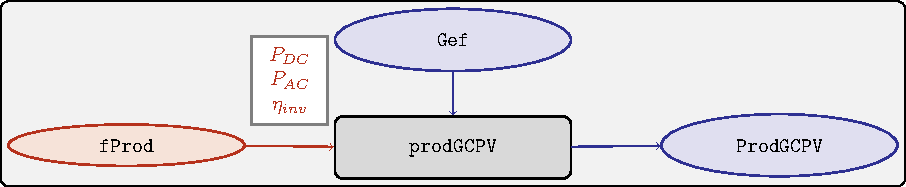
\includegraphics[keepaspectratio,width=\textwidth,height=\textheight]{figuras/prodgcpv.pdf}
\caption{Estimación de la producción eléctrica de un SFCR mediante la función \texttt{prodGCPV}, la cual emplea la función \texttt{fProd} para el computo de la potencia a la entrada (\(P_{DC}\)), a la salida (\(P_{AC}\)) y el rendimiento (\(\eta_{inv}\)) del inversor. \label{fig:prodgcpv}}
\end{figure}
\begin{itemize}
\item \texttt{fProd}: simula el comportamiento de un sistema fotovoltaico conectado a red bajo diferentes condiciones de temperatura e irradiancia. Tiene los siguientes argumentos:
\begin{itemize}
\item \texttt{inclin}: puede ser tanto un objeto de clase \texttt{Gef} como un \texttt{data.frame} (o \texttt{data.table}). Sin embargo, si es un \texttt{data.frame}, debe contener como mínimo una columna para \texttt{Gef} y otra para \texttt{Ta}
\item \texttt{module}: una lista de valores numéricos con la información sobre el módulo fotovoltaico:
\begin{itemize}
\item \texttt{Vocn}: tensión de circuito abierto en STC (\(V_{oc}^*\))(condiciones estandar de médida). Por defecto, tiene un valor de \(57.2V\).
\item \texttt{Iscn}: corriente de cortocircuito en STC (\(I_{sc}^*\)). Por defecto, tiene un valor de \(4.7A\).
\item \texttt{Vmn}: tensión en el punto de máxima potencia en STC (\(I_{MPP}^*\)). Por defecto, tiene un valor de \(46.08V\).
\item \texttt{Imn}: corriente de cortocircuito en STC (\(I_{MPP}^*\)). Por defecto, tiene un valor de \(4.35A\)).
\item \texttt{Ncs}: número de células en serie dentro del módulo. Por defecto, tiene un valor de 96.
\item \texttt{Ncp}: número de células en paralelo dentro del módulo. Por defecto, tiene un valor de 1.
\item \texttt{CoefVT}: coeficiente de disminución de la tensión  de cada célula con la temperatura (\(dV_{oc}/dT_c\)). Por defecto, tiene un valor de \(-0.0023 V/^\circ C\).
\item \texttt{TONC}: temperatura de operación nominal de célula (\(TONC\)). Por defecto, tiene un valor de \(47^\circ C\).
\end{itemize}
\item \texttt{generator}: lista de valores numéricos con la información sobre el generador:
\begin{itemize}
\item \texttt{Nms}: número de módulos en serie. Por defecto, tiene un valor de 12.
\item \texttt{Nmp}: número de módulos en paralelo. Por defecto, tiene un valor de 11.
\end{itemize}
\item \texttt{inverter}: lista de valores númericos con la información del inversor DC/AC.
\begin{itemize}
\item \texttt{Ki}: coeficientes de la curva de eficiencia del inversor. Se puede presentar en un vector de 3 valores (por defecto, \texttt{c(0.01, 0.025, 0.05)}) o una matriz de 9 valores (si tiene dependencia del voltage).
\item \texttt{Pinv}: potencia nominal del inversor. Por defecto, tiene un valor de \(25000 W\).
\item \texttt{Vmin}: mínima tensión del rango MPP del inversor. Por defecto, tiene un valor de \(420V\).
\item \texttt{Vmax}: máxima tensión del rango MPP del inversor. Por defecto, tiene un valor de \(750V\).
\item \texttt{Gumb}: irradiancia umbral de funcionamienot del inversor. Por defecto, tiene un valor de \(20W/m^2\).
\end{itemize}
\item \texttt{effSys}: una lista de valores numéricos con la información sobre las pérdidas del sistema.
\begin{itemize}
\item \texttt{ModQual}: tolerancia media del set de módulos (\(\%\)). Por defecto, tiene un valor de 3.
\item \texttt{ModDisp}: pérdidas por dispersión en los módulos (\(\%\)). Por defecto, tiene un valor de 2.
\item \texttt{OhmDC}: pérdidas por efecto Joule en el cableado de DC (\(\%\)). Por defecto, tiene un valor de 1.5.
\item \texttt{OhmAC}: pérdidas por efecto Joule en el cableado de AC (\(\%\)). Por defecto, tiene un valor de 1.5.
\item \texttt{MPP}: error promedio del algoritmo de búsqueda del MPP del inversor (\(\%\)). Por defecto, tiene un valor de 1.
\item \texttt{TrafoMT}: pérdidas por el transformador MT (\(\%\)). Por defecto, tiene un valor de 1.
\item \texttt{Disp}: pérdidas por las paradas del sistema (\(\%\)). Por defecto, tiene un valor de 0.5.
\end{itemize}
\end{itemize}
\end{itemize}
\begin{lstlisting}[numbers=left,language=r,label= ,caption= ,captionpos=b]
inclin <- calcGef(lat, dataRad = prom, keep.night = FALSE)
module <- list(Vocn=57.6, Iscn=4.7, Vmn=46.08, Imn=4.35,
               Ncs=96, Ncp=1, CoefVT=0.0023, TONC=47)
generator <- list(Nms=12, Nmp=11)
inverter <- list(Ki=c(0.01, 0.025, 0.05), Pinv=25000,
                 Vmin=420, Vmax=750, Gumb=20)
effSys <- list(ModQual=3, ModDisp=2, OhmDC=1.5, OhmAC=1.5,
               MPP=1, TrafoMT=1, Disp=0.5)
prod <- fProd(inclin = inclin, module = module,
              generator = generator, inverter = inverter,
              effSys = effSys)
show(prod)
\end{lstlisting}

\begin{verbatim}
                   Dates       Tc      Voc       Isc     Vmpp      Impp      Vdc       Idc       Pac
                  <POSc>    <num>    <num>     <num>    <num>     <num>    <num>     <num>     <num>
  1: 2024-01-17 08:00:00 15.27689 716.9624  8.083413 607.4640  7.620135 607.4640  7.620135  3796.209
  2: 2024-01-17 09:00:00 21.43284 700.6516 17.513415 583.9663 16.433741 583.9663 16.433741  8053.912
  3: 2024-01-17 10:00:00 27.23609 685.2753 26.403138 562.0190 24.658263 562.0190 24.658263 11650.920
  4: 2024-01-17 11:00:00 31.48724 674.0114 32.915263 546.0746 30.625265 546.0746 30.625265 14041.629
  5: 2024-01-17 12:00:00 33.33104 669.1261 35.739693 539.1958 33.196772 539.1958 33.196772 15016.481
 ---                                                                                                
141: 2024-12-13 12:00:00 33.94967 667.4869 28.721724 542.4718 26.706186 542.4718 26.706186 12177.570
142: 2024-12-13 13:00:00 32.55186 671.1906 26.580476 547.6944 24.746716 547.6944 24.746716 11395.331
143: 2024-12-13 14:00:00 29.08872 680.3665 21.275466 560.6878 19.868077 560.6878 19.868077  9362.088
144: 2024-12-13 15:00:00 24.29331 693.0724 13.929608 578.8034 13.059814 578.8034 13.059814  6316.091
145: 2024-12-13 16:00:00 19.21305 706.5331  6.147403 598.1441  5.786102 598.1441  5.786102  2784.663
           Pdc      EffI
         <num>     <num>
  1:  4290.940 0.9118076
  2:  8895.974 0.9330800
  3: 12846.437 0.9347232
  4: 15502.477 0.9335163
  5: 16592.492 0.9327431
 ---                    
141: 13429.451 0.9345615
142: 12563.918 0.9347755
143: 10326.335 0.9343983
144:  7007.083 0.9290019
145:  3208.198 0.8945754
\end{verbatim}

Esta función brinda estos datos a la función \texttt{prodGCPV} para que produzca un objeto de clase \texttt{ProdGCPV} como resultado. Esta función tiene como argumentos principales los mismo que \texttt{calcGef}, ya que parte de un objeto tipo \texttt{Gef}, y los argumentos de la función \texttt{fProd}.
\begin{lstlisting}[numbers=left,language=r,label= ,caption= ,captionpos=b]
prodFixed <- prodGCPV(lat, modeTrk = 'fixed', dataRad = prom)
show(prodFixed)
\end{lstlisting}

\begin{verbatim}
Object of class  ProdGCPV 

Source of meteorological information: prom- 

Latitude of source:  37.2 degrees
Latitude for calculations:  37.2 degrees

Monthly avarages:
        Dates       Eac       Edc       Yf
       <char>     <num>     <num>    <num>
 1: Jan. 2024  95.36291 105.62767 3.604158
 2: Feb. 2024 101.50809 112.56166 3.836410
 3: Mar. 2024 110.26945 122.11835 4.167538
 4: Apr. 2024 124.53728 138.29836 4.706778
 5: May. 2024 131.48629 145.91065 4.969410
 6: Jun. 2024 135.89421 150.78725 5.136003
 7: Jul. 2024 134.98501 149.81246 5.101641
 8: Aug. 2024 130.25804 144.39951 4.922989
 9: Sep. 2024 119.91911 132.77648 4.532238
10: Oct. 2024  96.49455 106.99182 3.646928
11: Nov. 2024  90.17737  99.88152 3.408175
12: Dec. 2024  73.89289  81.80967 2.792718

Yearly values:
   Dates     Eac      Edc       Yf
   <int>   <num>    <num>    <num>
1:  2024 41014.8 45473.37 1550.119
-----------------
Mode of tracking:  fixed 
    Inclination:  27.2 
    Orientation:  0 
-----------------
Generator:
    Modules in series:  12 
    Modules in parallel:  11 
    Nominal power (kWp):  26.5
\end{verbatim}

\begin{lstlisting}[numbers=left,language=r,label= ,caption= ,captionpos=b]
prod2x <- prodGCPV(lat, modeTrk = 'two', dataRad = prom)
show(prod2x)
\end{lstlisting}

\begin{verbatim}
Object of class  ProdGCPV 

Source of meteorological information: prom- 

Latitude of source:  37.2 degrees
Latitude for calculations:  37.2 degrees

Monthly avarages:
        Dates      Eac      Edc       Yf
       <char>    <num>    <num>    <num>
 1: Jan. 2024 138.6806 153.2566 5.241314
 2: Feb. 2024 143.4987 158.5247 5.423408
 3: Mar. 2024 151.8477 167.7311 5.738952
 4: Apr. 2024 178.6717 197.4274 6.752741
 5: May. 2024 200.8888 222.0523 7.592419
 6: Jun. 2024 223.9959 247.6903 8.465728
 7: Jul. 2024 214.2749 236.9628 8.098332
 8: Aug. 2024 194.6043 215.1439 7.354902
 9: Sep. 2024 168.9824 186.7349 6.386542
10: Oct. 2024 132.2995 146.0747 5.000145
11: Nov. 2024 128.5783 141.9871 4.859507
12: Dec. 2024 102.9116 113.5613 3.889454

Yearly values:
   Dates      Eac      Edc       Yf
   <int>    <num>    <num>    <num>
1:  2024 60369.04 66710.67 2281.595
-----------------
Mode of tracking:  two 
    Inclination limit: 90 
-----------------
Generator:
    Modules in series:  12 
    Modules in parallel:  11 
    Nominal power (kWp):  26.5
\end{verbatim}

\begin{lstlisting}[numbers=left,language=r,label= ,caption= ,captionpos=b]
prodHoriz <- prodGCPV(lat, modeTrk = 'horiz', dataRad = prom)
show(prodHoriz)
\end{lstlisting}

\begin{verbatim}
Object of class  ProdGCPV 

Source of meteorological information: prom- 

Latitude of source:  37.2 degrees
Latitude for calculations:  37.2 degrees

Monthly avarages:
        Dates       Eac       Edc       Yf
       <char>     <num>     <num>    <num>
 1: Jan. 2024  99.43006 109.66074 3.757873
 2: Feb. 2024 116.24796 128.22238 4.393490
 3: Mar. 2024 137.39485 151.61074 5.192719
 4: Apr. 2024 172.03044 189.97488 6.501741
 5: May. 2024 196.91337 217.61396 7.442169
 6: Jun. 2024 219.15566 242.31468 8.282797
 7: Jul. 2024 210.33644 232.56087 7.949482
 8: Aug. 2024 189.03576 208.87993 7.144442
 9: Sep. 2024 156.22909 172.44519 5.904542
10: Oct. 2024 110.69482 122.11859 4.183614
11: Nov. 2024  94.40734 104.14723 3.568043
12: Dec. 2024  69.94550  77.30532 2.643529

Yearly values:
   Dates      Eac      Edc       Yf
   <int>    <num>    <num>    <num>
1:  2024 54052.14 59697.16 2042.854
-----------------
Mode of tracking:  horiz 
    Inclination limit: 90 
-----------------
Generator:
    Modules in series:  12 
    Modules in parallel:  11 
    Nominal power (kWp):  26.5
\end{verbatim}

\section{Producción eléctrica de un SFB}
\label{sec:org7e6dc82}
De igual forma que en el apartado anterior, se puede estimar la producción eléctrica de un sistema fotovoltaico de bombeo.

Como se puede ver en la figura \ref{fig:prodpvps}, \texttt{prodPVPS} funciona gracias a la siguiente función:
\begin{figure}[htbp]
\centering
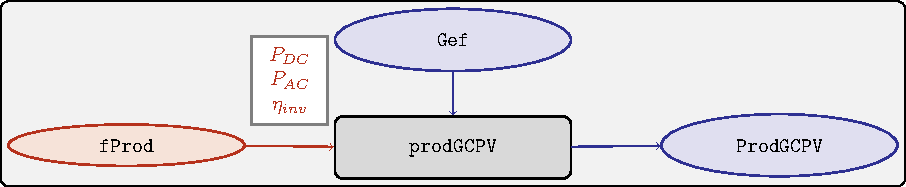
\includegraphics[keepaspectratio,width=\textwidth,height=0.5\textheight]{figuras/prodpvps.pdf}
\caption{Estimación de la producción eléctrica de un SFB mediante la función \texttt{prodPVPS}, la cual emplea la función \texttt{fPump} para el computo del rendimiento de las diferentes parte de una bomba centrífuga alimentada por un convertidor de frecuencia. \label{fig:prodpvps}}
\end{figure}
\begin{itemize}
\item \texttt{fPump}: calcula el rendimiento de las diferentes partes de una bomba centrífuga alimentada por un convertidor de frecuencia siguiendo las leyes de afinidad. Tiene solo dos argumentos:
\begin{itemize}
\item \texttt{pump}: lista que contiene los parametros de la bomba que va a ser simulada. Puede ser una fila de \texttt{pumpCoef}:
\begin{lstlisting}[numbers=left,language=r,label= ,caption= ,captionpos=b]
CoefSP8A44 <- pumpCoef[Qn == 8 & stages == 44]
show(CoefSP8A44)
\end{lstlisting}

\begin{verbatim}
      Qn stages  Qmax   Pmn         a         b      c     g     h     i       j     k      l
   <int>  <int> <num> <int>     <num>     <num>  <num> <num> <num> <num>   <num> <num>  <num>
1:     8     44    12  7500 0.1043011 -0.101288 -0.726 -0.24  0.42  0.64 -0.0058 0.095 0.2013
\end{verbatim}

\item \texttt{H}: el salto manometrico total.
\end{itemize}
\begin{lstlisting}[numbers=left,language=r,label= ,caption= ,captionpos=b]
fSP8A44 <- fPump(pump = CoefSP8A44, H = 40)
\end{lstlisting}

Obtiene como resultado los siguientes valores y funciones:
\begin{itemize}
\item \texttt{lim}: rango de valores de la potencia eléctrica de salida.
\begin{lstlisting}[numbers=left,language=r,label= ,caption= ,captionpos=b]
show(fSP8A44$lim)
\end{lstlisting}

\begin{verbatim}
[1]  190.100 4084.218
\end{verbatim}

\item \texttt{fQ}: función que relaciona el caudal con la potencia eléctrica.
\begin{lstlisting}[numbers=left,language=r,label= ,caption= ,captionpos=b]
show(fSP8A44$fQ)
\end{lstlisting}

\begin{verbatim}
function (x, deriv = 0L) 
{
    deriv <- as.integer(deriv)
    if (deriv < 0L || deriv > 3L) 
	stop("'deriv' must be between 0 and 3")
    if (deriv > 0L) {
	z0 <- double(z$n)
	z[c("y", "b", "c")] <- switch(deriv, list(y = z$b, b = 2 * 
	    z$c, c = 3 * z$d), list(y = 2 * z$c, b = 6 * z$d, 
	    c = z0), list(y = 6 * z$d, b = z0, c = z0))
	z[["d"]] <- z0
    }
    res <- .splinefun(x, z)
    if (deriv > 0 && z$method == 2 && any(ind <- x <= z$x[1L])) 
	res[ind] <- ifelse(deriv == 1, z$y[1L], 0)
    res
}
<bytecode: 0x00000241cd298748>
<environment: 0x00000241cd29cda0>
\end{verbatim}

\item \texttt{fPb}: función que relaciona la potencia del eje de la bomba con la potencia eléctrica del motor.
\begin{lstlisting}[numbers=left,language=r,label= ,caption= ,captionpos=b]
show(fSP8A44$fPb)
\end{lstlisting}

\begin{verbatim}
function (x, deriv = 0L) 
{
    deriv <- as.integer(deriv)
    if (deriv < 0L || deriv > 3L) 
	stop("'deriv' must be between 0 and 3")
    if (deriv > 0L) {
	z0 <- double(z$n)
	z[c("y", "b", "c")] <- switch(deriv, list(y = z$b, b = 2 * 
	    z$c, c = 3 * z$d), list(y = 2 * z$c, b = 6 * z$d, 
	    c = z0), list(y = 6 * z$d, b = z0, c = z0))
	z[["d"]] <- z0
    }
    res <- .splinefun(x, z)
    if (deriv > 0 && z$method == 2 && any(ind <- x <= z$x[1L])) 
	res[ind] <- ifelse(deriv == 1, z$y[1L], 0)
    res
}
<bytecode: 0x00000241cd298748>
<environment: 0x00000241cd311e08>
\end{verbatim}

\item \texttt{fPh}: función que relaciona la potencia hidráulica con la potencia eléctrica del motor.
\begin{lstlisting}[numbers=left,language=r,label= ,caption= ,captionpos=b]
show(fSP8A44$fPh)
\end{lstlisting}

\begin{verbatim}
function (x, deriv = 0L) 
{
    deriv <- as.integer(deriv)
    if (deriv < 0L || deriv > 3L) 
	stop("'deriv' must be between 0 and 3")
    if (deriv > 0L) {
	z0 <- double(z$n)
	z[c("y", "b", "c")] <- switch(deriv, list(y = z$b, b = 2 * 
	    z$c, c = 3 * z$d), list(y = 2 * z$c, b = 6 * z$d, 
	    c = z0), list(y = 6 * z$d, b = z0, c = z0))
	z[["d"]] <- z0
    }
    res <- .splinefun(x, z)
    if (deriv > 0 && z$method == 2 && any(ind <- x <= z$x[1L])) 
	res[ind] <- ifelse(deriv == 1, z$y[1L], 0)
    res
}
<bytecode: 0x00000241cd298748>
<environment: 0x00000241cd32cd30>
\end{verbatim}

\item \texttt{fFreq}: función que relaciona la frecuencia con la potencia eléctrica del motor.
\begin{lstlisting}[numbers=left,language=r,label= ,caption= ,captionpos=b]
show(fSP8A44$fFreq)
\end{lstlisting}

\begin{verbatim}
function (x, deriv = 0L) 
{
    deriv <- as.integer(deriv)
    if (deriv < 0L || deriv > 3L) 
	stop("'deriv' must be between 0 and 3")
    if (deriv > 0L) {
	z0 <- double(z$n)
	z[c("y", "b", "c")] <- switch(deriv, list(y = z$b, b = 2 * 
	    z$c, c = 3 * z$d), list(y = 2 * z$c, b = 6 * z$d, 
	    c = z0), list(y = 6 * z$d, b = z0, c = z0))
	z[["d"]] <- z0
    }
    res <- .splinefun(x, z)
    if (deriv > 0 && z$method == 2 && any(ind <- x <= z$x[1L])) 
	res[ind] <- ifelse(deriv == 1, z$y[1L], 0)
    res
}
<bytecode: 0x00000241cd298748>
<environment: 0x00000241cd2be128>
\end{verbatim}
\end{itemize}

Se pueden realizar operaciones con este objeto:
\begin{lstlisting}[numbers=left,language=r,label= ,caption= ,captionpos=b]
SP8A44 = with(fSP8A44,{
  Pac = seq(lim[1],lim[2],l=10)
  Pb = fPb(Pac)
  etam = Pb/Pac
  Ph = fPh(Pac)
  etab = Ph/Pb
  f = fFreq(Pac)
  Q = fQ(Pac)
  result = data.table(Q,Pac,Pb,Ph,etam,etab,f)})
show(SP8A44)
\end{lstlisting}

\begin{verbatim}
	     Q       Pac        Pb         Ph      etam      etab        f
	 <num>     <num>     <num>      <num>     <num>     <num>    <num>
 1:  0.3133325  190.1000  124.8346   34.15325 0.6566786 0.2735880 20.47033
 2:  2.0718468  622.7798  429.6728  225.83130 0.6899274 0.5255890 22.33036
 3:  4.0764128 1055.4595  752.8970  444.32900 0.7133358 0.5901591 25.51459
 4:  5.6406747 1488.1393 1087.3665  614.83354 0.7306887 0.5654336 28.73213
 5:  6.9474993 1920.8190 1429.7984  757.27743 0.7443692 0.5296393 31.78514
 6:  8.1028841 2353.4988 1778.0156  883.21437 0.7554776 0.4967416 34.69527
 7:  9.1607296 2786.1786 2130.4683  998.51953 0.7646560 0.4686855 37.49608
 8: 10.1514390 3218.8583 2486.0213 1106.50685 0.7723301 0.4450915 40.21428
 9: 11.0937480 3651.5381 2843.8295 1209.21854 0.7788032 0.4252078 42.86977
10: 12.0000000 4084.2179 3203.2578 1308.00000 0.7843014 0.4083343 45.47737
\end{verbatim}

Está función entrega todos estos resultados a \texttt{prodPVPS} la cual calcula los resultados en base a la potencia del generador a simular, y devuleve un objeto de clase \texttt{ProdPVPS}.
\begin{lstlisting}[numbers=left,language=r,label= ,caption= ,captionpos=b]
prodsfb <- prodPVPS(lat, modeTrk = 'fixed', dataRad = prom,
                    pump = CoefSP8A44, H = 40, Pg = SP8A44$Pac[10])
show(prodsfb)
\end{lstlisting}

\begin{verbatim}
Object of class  ProdPVPS 

Source of meteorological information: prom- 

Latitude of source:  37.2 degrees
Latitude for calculations:  37.2 degrees

Monthly avarages:
	Dates      Eac       Qd       Yf
       <char>    <num>    <num>    <num>
 1: Jan. 2024 14.07129 50.46621 3.445284
 2: Feb. 2024 15.43701 54.71213 3.779675
 3: Mar. 2024 17.00102 59.68995 4.162613
 4: Apr. 2024 19.39135 67.24260 4.747874
 5: May. 2024 20.65046 71.34195 5.056160
 6: Jun. 2024 21.63947 74.27359 5.298315
 7: Jul. 2024 22.62915 76.77927 5.540633
 8: Aug. 2024 22.17136 75.07166 5.428546
 9: Sep. 2024 19.61622 67.34348 4.802932
10: Oct. 2024 14.92078 53.24853 3.653277
11: Nov. 2024 13.75298 49.50040 3.367348
12: Dec. 2024 11.21349 40.90244 2.745567

Yearly values:
   Dates      Eac       Qd       Yf
   <int>    <num>    <num>    <num>
1:  2024 6482.059 22589.95 1587.099
-----------------
Mode of tracking:  fixed 
    Inclination:  27.2 
    Orientation:  0 
-----------------
Pump:
    Qn:  8 
    Stages:  44 
Height (m):  40 
Generator (Wp):  4084.218
\end{verbatim}
\end{itemize}

\section{Optimización de distancias}
\label{sec:org20d1f91}
\label{optimizacion-distancias}
Por último, el paquete \texttt{solaR2} contiene una función que permite calcular un conjunto de combinaciones de distancias entre los elementos de un sistema fotovoltaico conectado a red, con el fin de que el usuario posteriormente pueda optar cual es la opción mas rentable en base a los precios del cableado y de la ocupación del terreno.

Esta función es \texttt{optimShd}, la cual en base a una resolución (determinada por el argumento \texttt{res}, el cual, indica el incremento de la secuencia de distancias) obtiene la producción de cada combinación y la plasma en un objeto de clase \texttt{Shade}.
\begin{lstlisting}[numbers=left,language=r,label= ,caption= ,captionpos=b]
struct2x <- list(W = 23.11, L = 9.8, Nrow = 2, Ncol = 3)
dist2x <- list(Lew = c(30, 45), Lns = c(20, 40))
ShdM2x <- optimShd(lat, dataRad = prom, modeTrk = 'two',
                   modeShd = c('area', 'prom'),
                   distances = dist2x, struct = struct2x,
                   res = 5,
                   prog = FALSE) #Se quita la barra de progreso
show(ShdM2x)
\end{lstlisting}

\begin{verbatim}
Object of class  Shade 

Source of meteorological information: prom- 

Latitude of source:  37.2 degrees
Latitude for calculations:  37.2 degrees

Monthly avarages:
Dimensions of structure:
$W
[1] 23.11

$L
[1] 9.8

$Nrow
[1] 2

$Ncol
[1] 3

Shade calculation mode:
[1] "area" "prom"
Productivity without shadows:
Object of class  ProdGCPV 

Source of meteorological information: prom- 

Latitude of source:  37.2 degrees
Latitude for calculations:  37.2 degrees

Monthly avarages:
        Dates      Eac      Edc       Yf
       <char>    <num>    <num>    <num>
 1: Jan. 2024 138.6806 153.2566 5.241314
 2: Feb. 2024 143.4987 158.5247 5.423408
 3: Mar. 2024 151.8477 167.7311 5.738952
 4: Apr. 2024 178.6717 197.4274 6.752741
 5: May. 2024 200.8888 222.0523 7.592419
 6: Jun. 2024 223.9959 247.6903 8.465728
 7: Jul. 2024 214.2749 236.9628 8.098332
 8: Aug. 2024 194.6043 215.1439 7.354902
 9: Sep. 2024 168.9824 186.7349 6.386542
10: Oct. 2024 132.2995 146.0747 5.000145
11: Nov. 2024 128.5783 141.9871 4.859507
12: Dec. 2024 102.9116 113.5613 3.889454

Yearly values:
   Dates      Eac      Edc       Yf
   <int>    <num>    <num>    <num>
1:  2024 60369.04 66710.67 2281.595
-----------------
Mode of tracking:  two 
    Inclination limit: 90 
-----------------
Generator:
    Modules in series:  12 
    Modules in parallel:  11 
    Nominal power (kWp):  26.5 

Summary of results:
      Lew             Lns           H           FS               GRR              Yf      
 Min.   :30.00   Min.   :20   Min.   :0   Min.   :0.01509   Min.   :2.649   Min.   :2104  
 1st Qu.:33.75   1st Qu.:25   1st Qu.:0   1st Qu.:0.02223   1st Qu.:3.946   1st Qu.:2192  
 Median :37.50   Median :30   Median :0   Median :0.02870   Median :4.802   Median :2216  
 Mean   :37.50   Mean   :30   Mean   :0   Mean   :0.03463   Mean   :4.967   Mean   :2203  
 3rd Qu.:41.25   3rd Qu.:35   3rd Qu.:0   3rd Qu.:0.03945   3rd Qu.:6.016   3rd Qu.:2231  
 Max.   :45.00   Max.   :40   Max.   :0   Max.   :0.07769   Max.   :7.948   Max.   :2247
\end{verbatim}

\begin{lstlisting}[numbers=left,language=r,label= ,caption= ,captionpos=b]
structHoriz = list(L = 4.83)
distHoriz = list(Lew = structHoriz$L * c(2,5))
Shd12HorizBT <- optimShd(lat = lat, dataRad = prom,
                         modeTrk = 'horiz',
                         betaLim = 60,
                         distances = distHoriz, res = 2,
                         struct = structHoriz,
                         modeShd = 'bt',
                         prog = FALSE) #Se quita la barra de progreso
show(Shd12HorizBT)
\end{lstlisting}

\begin{verbatim}
Object of class  Shade 

Source of meteorological information: prom- 

Latitude of source:  37.2 degrees
Latitude for calculations:  37.2 degrees

Monthly avarages:
Dimensions of structure:
$L
[1] 4.83

Shade calculation mode:
[1] "bt"
Productivity without shadows:
Object of class  ProdGCPV 

Source of meteorological information: prom- 

Latitude of source:  37.2 degrees
Latitude for calculations:  37.2 degrees

Monthly avarages:
        Dates       Eac       Edc       Yf
       <char>     <num>     <num>    <num>
 1: Jan. 2024  97.48365 107.53823 3.684309
 2: Feb. 2024 114.31569 126.11751 4.320462
 3: Mar. 2024 135.67629 149.74056 5.127767
 4: Apr. 2024 170.28530 188.06424 6.435785
 5: May. 2024 194.83600 215.33865 7.363657
 6: Jun. 2024 216.37522 239.26256 8.177713
 7: Jul. 2024 208.20413 230.21074 7.868894
 8: Aug. 2024 187.19428 206.84745 7.074845
 9: Sep. 2024 154.37402 170.41035 5.834432
10: Oct. 2024 109.27362 120.57435 4.129901
11: Nov. 2024  92.82584 102.42576 3.508272
12: Dec. 2024  69.13228  76.42401 2.612794

Yearly values:
   Dates      Eac      Edc       Yf
   <int>    <num>    <num>    <num>
1:  2024 53386.77 58969.19 2017.707
-----------------
Mode of tracking:  horiz 
    Inclination limit: 60 
-----------------
Generator:
    Modules in series:  12 
    Modules in parallel:  11 
    Nominal power (kWp):  26.5 

Summary of results:
      Lew              H           FS               GRR              Yf      
 Min.   : 9.66   Min.   :0   Min.   :0.04804   Min.   :2.000   Min.   :1736  
 1st Qu.:13.16   1st Qu.:0   1st Qu.:0.05727   1st Qu.:2.725   1st Qu.:1824  
 Median :16.66   Median :0   Median :0.07295   Median :3.449   Median :1871  
 Mean   :16.66   Mean   :0   Mean   :0.08078   Mean   :3.449   Mean   :1855  
 3rd Qu.:20.16   3rd Qu.:0   3rd Qu.:0.09598   3rd Qu.:4.174   3rd Qu.:1902  
 Max.   :23.66   Max.   :0   Max.   :0.13968   Max.   :4.899   Max.   :1921
\end{verbatim}

\begin{lstlisting}[numbers=left,language=r,label= ,caption= ,captionpos=b]
structFixed = list(L = 5)
distFixed = list(D = structFixed$L*c(1,3))
Shd12Fixed <- optimShd(lat = lat, dataRad = prom,
                       modeTrk = 'fixed',
                       distances = distFixed, res = 2,
                       struct = structFixed,
                       modeShd = 'area',
                       prog = FALSE) #Se quita la barra de progreso
show(Shd12Fixed)
\end{lstlisting}

\begin{verbatim}
Object of class  Shade 

Source of meteorological information: prom- 

Latitude of source:  37.2 degrees
Latitude for calculations:  37.2 degrees

Monthly avarages:
Dimensions of structure:
$L
[1] 5

Shade calculation mode:
[1] "area"
Productivity without shadows:
Object of class  ProdGCPV 

Source of meteorological information: prom- 

Latitude of source:  37.2 degrees
Latitude for calculations:  37.2 degrees

Monthly avarages:
        Dates       Eac       Edc       Yf
       <char>     <num>     <num>    <num>
 1: Jan. 2024  95.36291 105.62767 3.604158
 2: Feb. 2024 101.50809 112.56166 3.836410
 3: Mar. 2024 110.26945 122.11835 4.167538
 4: Apr. 2024 124.53728 138.29836 4.706778
 5: May. 2024 131.48629 145.91065 4.969410
 6: Jun. 2024 135.89421 150.78725 5.136003
 7: Jul. 2024 134.98501 149.81246 5.101641
 8: Aug. 2024 130.25804 144.39951 4.922989
 9: Sep. 2024 119.91911 132.77648 4.532238
10: Oct. 2024  96.49455 106.99182 3.646928
11: Nov. 2024  90.17737  99.88152 3.408175
12: Dec. 2024  73.89289  81.80967 2.792718

Yearly values:
   Dates     Eac      Edc       Yf
   <int>   <num>    <num>    <num>
1:  2024 41014.8 45473.37 1550.119
-----------------
Mode of tracking:  fixed 
    Inclination:  27.2 
    Orientation:  0 
-----------------
Generator:
    Modules in series:  12 
    Modules in parallel:  11 
    Nominal power (kWp):  26.5 

Summary of results:
       D              H           FS                 GRR            Yf      
 Min.   : 5.0   Min.   :0   Min.   :0.0008477   Min.   :1.0   Min.   :1364  
 1st Qu.: 7.5   1st Qu.:0   1st Qu.:0.0015710   1st Qu.:1.5   1st Qu.:1511  
 Median :10.0   Median :0   Median :0.0038992   Median :2.0   Median :1544  
 Mean   :10.0   Mean   :0   Mean   :0.0269608   Mean   :2.0   Mean   :1508  
 3rd Qu.:12.5   3rd Qu.:0   3rd Qu.:0.0252790   3rd Qu.:2.5   3rd Qu.:1548  
 Max.   :15.0   Max.   :0   Max.   :0.1199180   Max.   :3.0   Max.   :1549
\end{verbatim}

\section{Métodos de visualización}
\label{sec:orgd70c2ae}
\label{sec:metodos-visualizacion}
Una vez creados todos los objetos, para mejorar la visualización de los mismos, \texttt{solaR2} cuanta con una serie de métodos que ayudan a la compresión de los datos obtenidos.

\subsection{Datos meteorológicos}
\label{sec:orgdf3f212}
La clase \texttt{Meteo} cuenta con un método para \texttt{xyplot}.
\begin{lstlisting}[numbers=left,language=r,label= ,caption= ,captionpos=b]
lat <- 37.2
G0dm = c(2.766,3.491,4.494,5.912,6.989,7.742,
         7.919,7.027,5.369,3.562,2.814,2.179) * 1000;
Ta = c(10, 14.1, 15.6, 17.2, 19.3, 21.2,
       28.4, 29.9, 24.3, 18.2, 17.2, 15.2)
BD <- readG0dm(G0dm = G0dm, Ta = Ta, lat = lat)
show(BD)
\end{lstlisting}

\begin{verbatim}
Object of class  Meteo 

Source of meteorological information: prom- 
Latitude of source:  37.2 degrees

Meteorological Data:
     Dates                 G0d             Ta       
 Min.   :2024-01-17   Min.   :2179   Min.   :10.00  
 1st Qu.:2024-04-07   1st Qu.:3322   1st Qu.:15.50  
 Median :2024-06-29   Median :4932   Median :17.70  
 Mean   :2024-07-01   Mean   :5022   Mean   :19.22  
 3rd Qu.:2024-09-25   3rd Qu.:6998   3rd Qu.:21.98  
 Max.   :2024-12-13   Max.   :7919   Max.   :29.90
\end{verbatim}

\begin{lstlisting}[numbers=left,language=r,label= ,caption= ,captionpos=b]
xyplot(BD)
\end{lstlisting}

\begin{center}
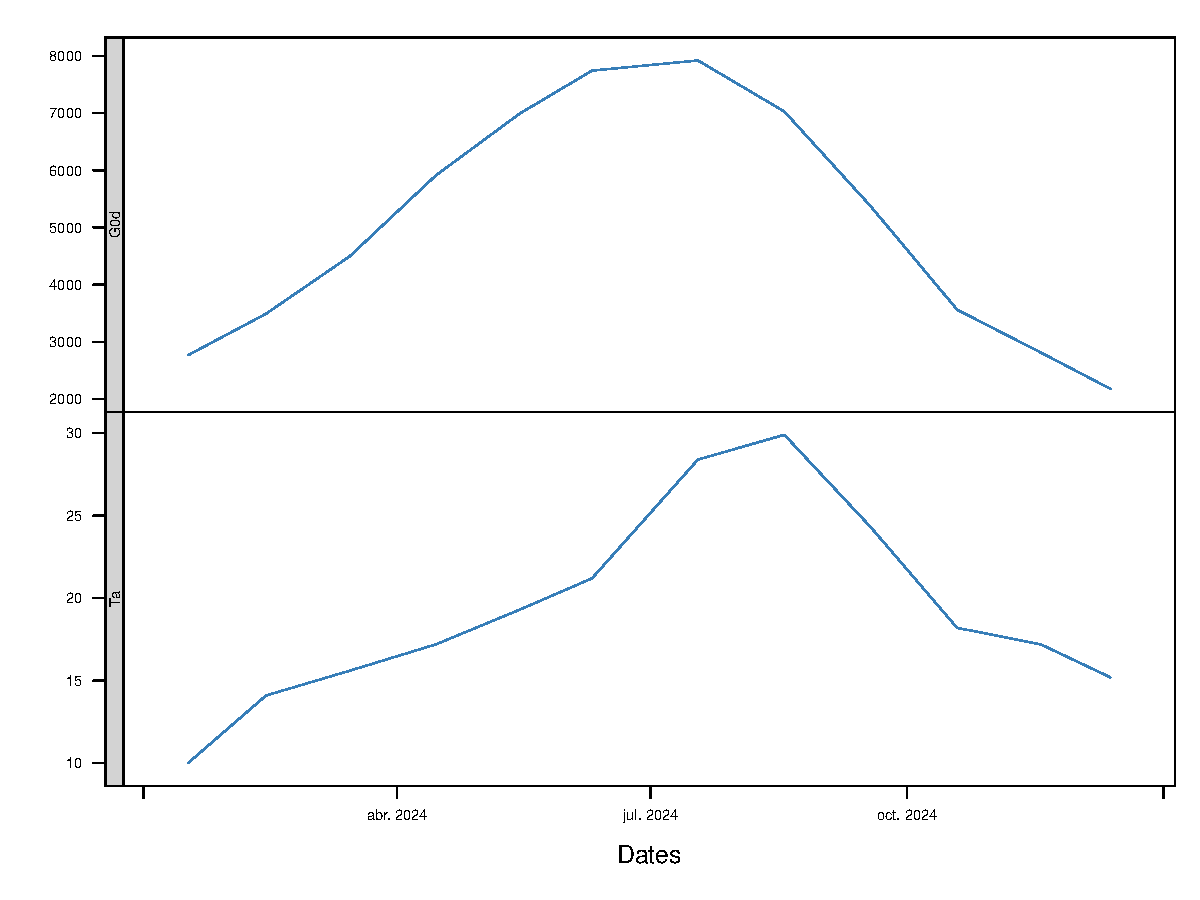
\includegraphics[width=0.8\textwidth]{figuras/codigo-meteo.pdf}
\end{center}

\subsection{Radiación en el plano horizontal}
\label{sec:org15a745b}
La clase \texttt{G0} cuenta con un método para \texttt{xyplot}.
\begin{lstlisting}[numbers=left,language=r,label= ,caption= ,captionpos=b]
g0 <- calcG0(lat, dataRad = BD)
show(g0)
\end{lstlisting}

\begin{verbatim}
Object of class  G0 

Source of meteorological information: prom- 

Latitude of source:  37.2 degrees
Latitude for calculations:  37.2 degrees

Monthly avarages:
        Dates   G0d      D0d      B0d
       <char> <num>    <num>    <num>
 1: Jan. 2024 2.766 0.941698 1.824302
 2: Feb. 2024 3.491 1.247146 2.243854
 3: Mar. 2024 4.494 1.671763 2.822237
 4: Apr. 2024 5.912 1.931146 3.980854
 5: May. 2024 6.989 2.023364 4.965636
 6: Jun. 2024 7.742 1.889994 5.852006
 7: Jul. 2024 7.919 1.624064 6.294936
 8: Aug. 2024 7.027 1.547591 5.479409
 9: Sep. 2024 5.369 1.540708 3.828292
10: Oct. 2024 3.562 1.374513 2.187487
11: Nov. 2024 2.814 1.006959 1.807041
12: Dec. 2024 2.179 0.926737 1.252263

Yearly values:
   Dates      G0d      D0d      B0d
   <int>    <num>    <num>    <num>
1:  2024 1839.365 540.6331 1298.732
\end{verbatim}

\begin{lstlisting}[numbers=left,language=r,label= ,caption= ,captionpos=b]
xyplot(g0)
\end{lstlisting}

\begin{center}
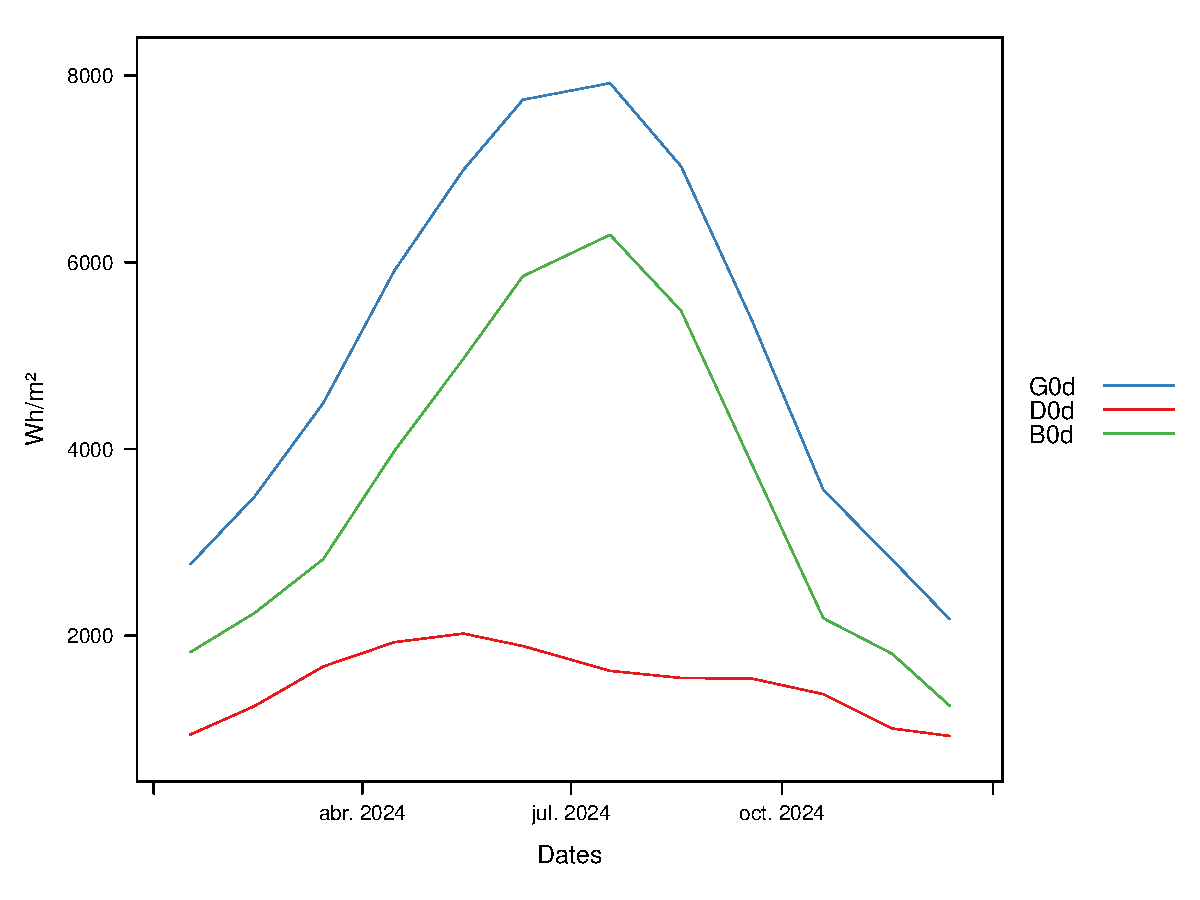
\includegraphics[width=0.8\textwidth]{figuras/codigo-g0.pdf}
\end{center}

Y con un método para \texttt{compare}.
\begin{lstlisting}[numbers=left,language=r,label= ,caption= ,captionpos=b]
g02 <- calcG0(lat, dataRad = list(G0dm = G0dm*0.95, Ta = Ta))
compare(g0, g02)
\end{lstlisting}

\begin{center}
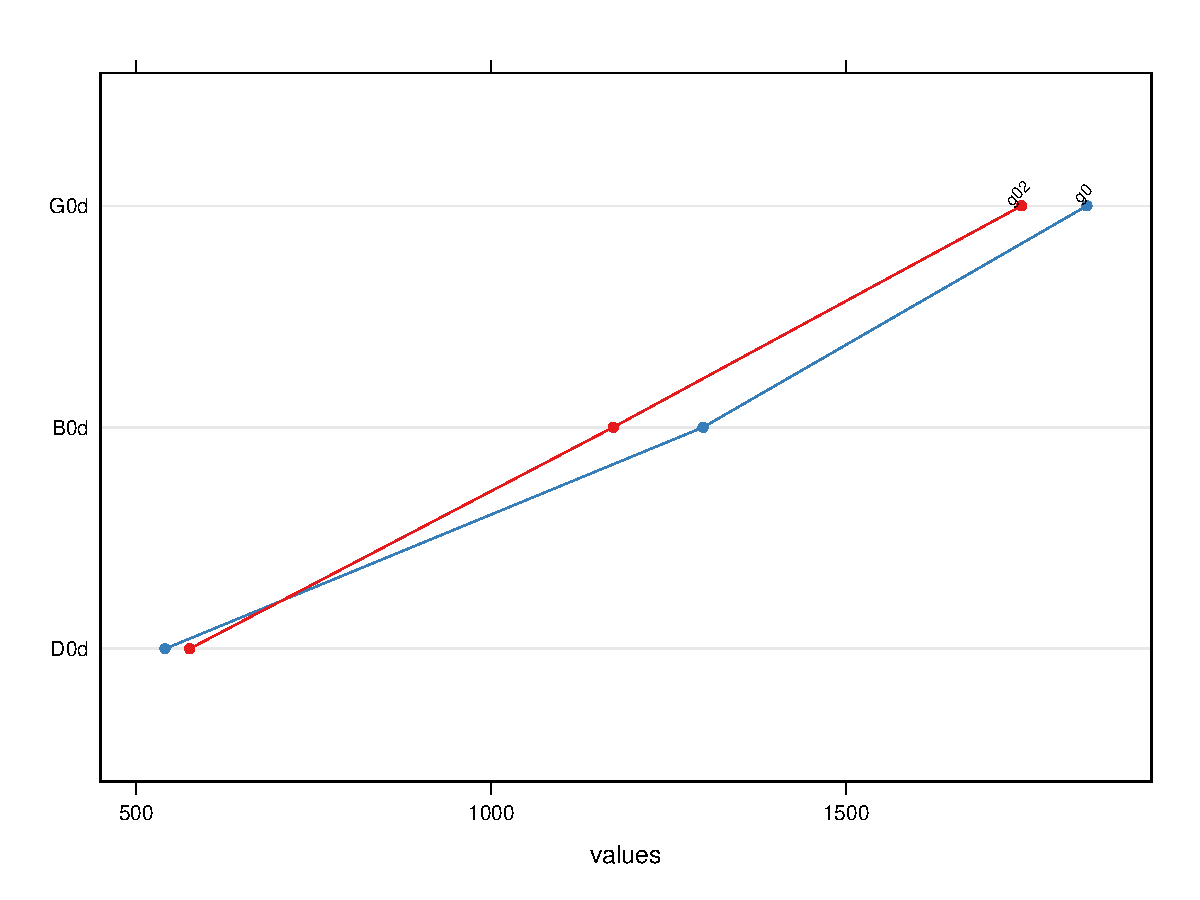
\includegraphics[width=0.8\textwidth]{figuras/codigo-g02.pdf}
\end{center}

\subsection{Radiación efectiva en el plano del generador}
\label{sec:org3ff504b}
La clase \texttt{Gef} cuenta con un método para \texttt{xyplot}.
\begin{lstlisting}[numbers=left,language=r,label= ,caption= ,captionpos=b]
gef <- calcGef(lat, dataRad = BD)
show(gef)
\end{lstlisting}

\begin{verbatim}
Object of class  Gef 

Source of meteorological information: prom- 

Latitude of source:  37.2 degrees
Latitude for calculations:  37.2 degrees

Monthly avarages:
        Dates       Bod       Bnd       Gd       Dd       Bd     Gefd     Defd     Befd
       <char>     <num>     <num>    <num>    <num>    <num>    <num>    <num>    <num>
 1: Jan. 2024  8.724907  4.924221 4.489744 1.200992 3.258164 4.220907 1.119517 3.080392
 2: Feb. 2024  9.592013  5.034287 4.919206 1.451954 3.428647 4.628492 1.352529 3.249460
 3: Mar. 2024 10.281308  5.163713 5.413543 1.779951 3.583896 5.101556 1.657369 3.410070
 4: Apr. 2024 10.527227  6.408617 6.282631 1.936897 4.280357 5.918787 1.803811 4.070094
 5: May. 2024 10.431853  7.617499 6.784202 1.937331 4.769584 6.371295 1.802060 4.516177
 6: Jun. 2024 10.291163  9.102430 7.173475 1.762326 5.325535 6.725684 1.639192 5.027718
 7: Jul. 2024 10.305302 10.037233 7.511733 1.533887 5.890275 7.058263 1.430322 5.567823
 8: Aug. 2024 10.394682  8.640959 7.295543 1.545089 5.672747 6.879777 1.443952 5.382478
 9: Sep. 2024 10.233884  6.698488 6.335591 1.647975 4.628244 5.982520 1.539552 4.402209
10: Oct. 2024  9.659077  4.546024 4.746760 1.538325 3.169044 4.470026 1.432213 3.010771
11: Nov. 2024  8.798687  4.638289 4.393712 1.244217 3.118376 4.134590 1.159756 2.953471
12: Dec. 2024  8.176298  3.439788 3.478125 1.128381 2.325648 3.274677 1.050626 2.207509

Yearly values:
   Dates      Bod      Bnd       Gd       Dd       Bd     Gefd     Defd     Befd
   <int>    <num>    <num>    <num>    <num>    <num>    <num>    <num>    <num>
1:  2024 3580.873 2326.882 2099.528 570.4317 1508.756 1975.745 531.5105 1430.271
-----------------
Mode of tracking:  fixed 
    Inclination:  27.2 
    Orientation:  0
\end{verbatim}

\begin{lstlisting}[numbers=left,language=r,label= ,caption= ,captionpos=b]
xyplot(gef)
\end{lstlisting}

\begin{center}
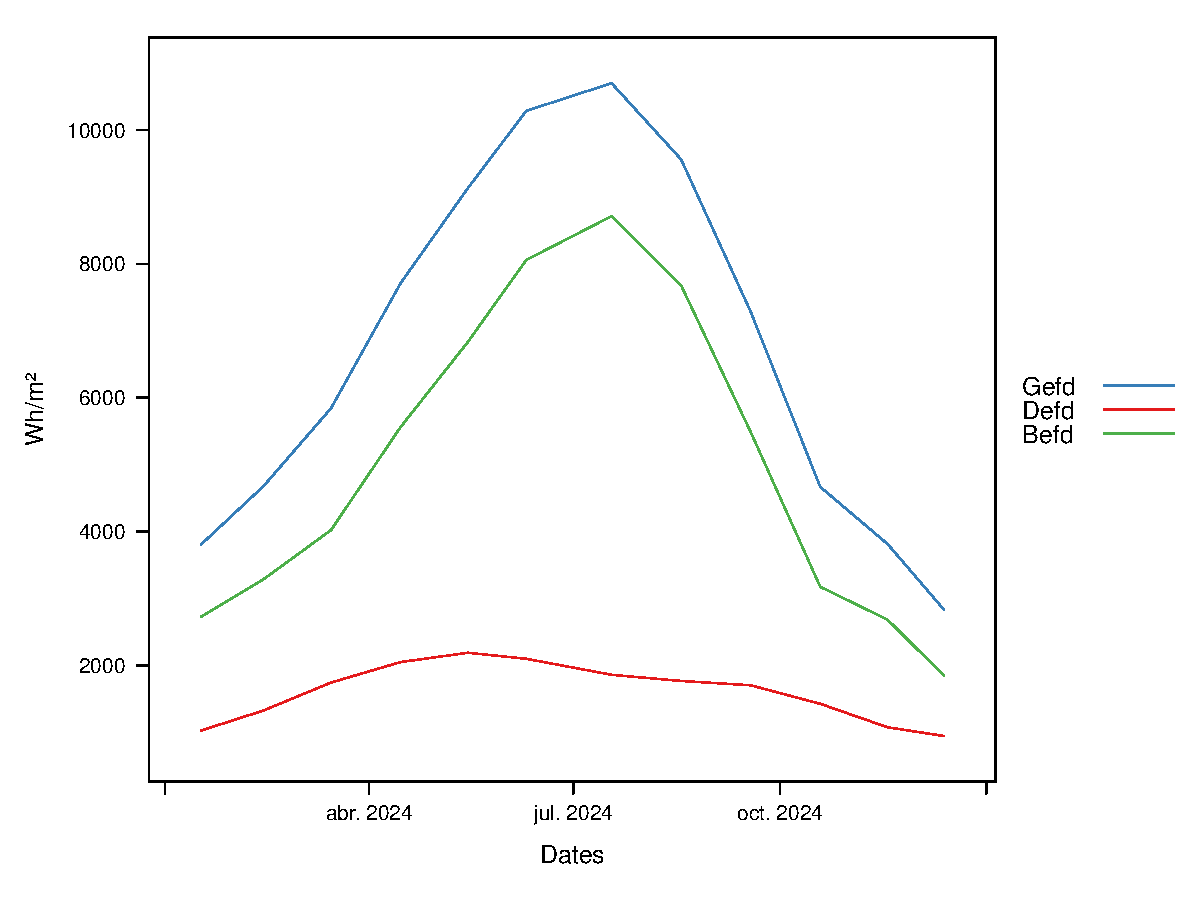
\includegraphics[width=0.8\textwidth]{figuras/codigo-gef.pdf}
\end{center}

Y con un método para \texttt{compare}.
\begin{lstlisting}[numbers=left,language=r,label= ,caption= ,captionpos=b]
gef2x <- calcGef(lat, modeTrk = 'two', dataRad = BD)
gefhoriz <- calcGef(lat, modeTrk = 'horiz', dataRad = BD)
compare(gef, gef2x, gefhoriz)
\end{lstlisting}

\begin{center}
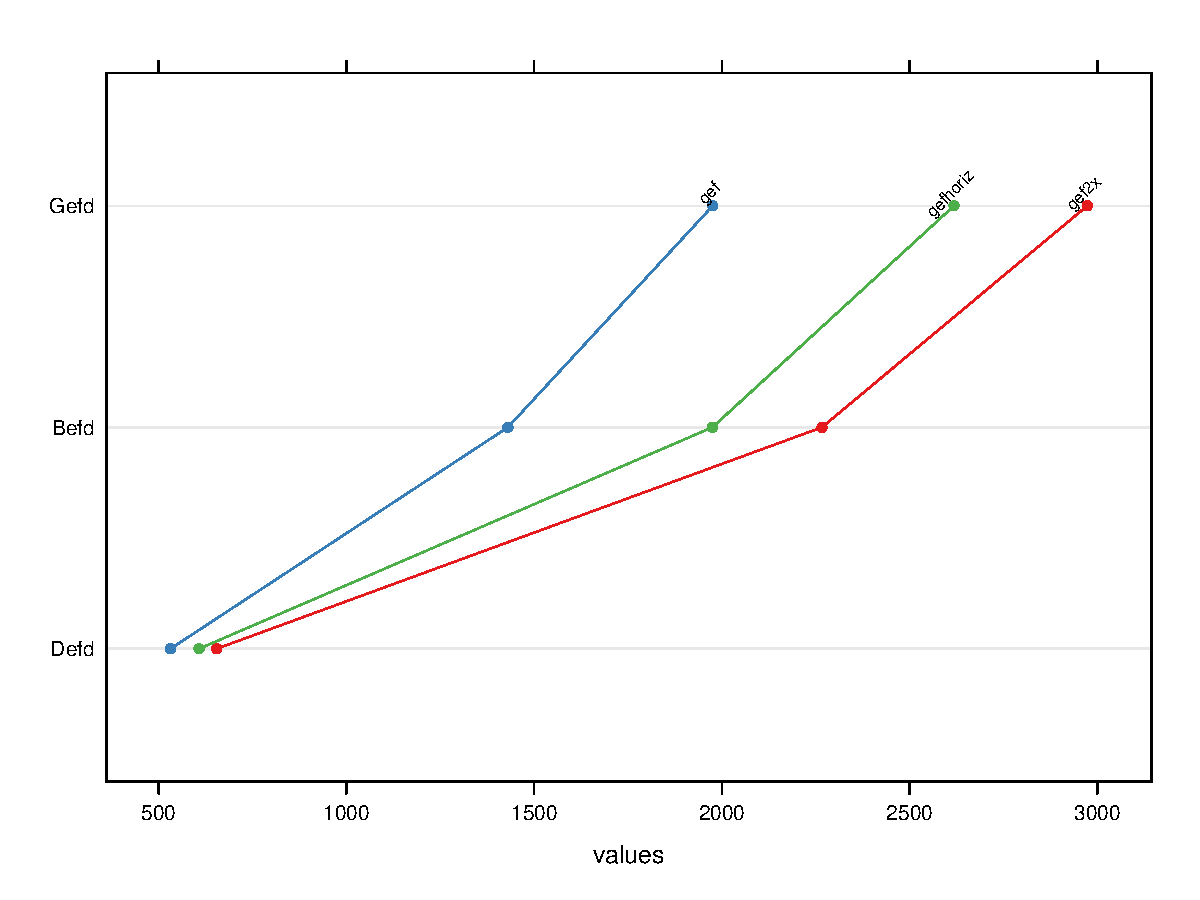
\includegraphics[width=0.8\textwidth]{figuras/codigo-gef2.pdf}
\end{center}


\subsection{Producción eléctrica de un SFCR}
\label{sec:orgcbe6d48}
La clase \texttt{ProdGCPV} cuenta con un método para \texttt{xyplot}.
\begin{lstlisting}[numbers=left,language=r,label= ,caption= ,captionpos=b]
prodFixed <- prodGCPV(lat, modeTrk = 'fixed', dataRad = BD)
show(prodFixed)
\end{lstlisting}

\begin{verbatim}
Object of class  ProdGCPV 

Source of meteorological information: prom- 

Latitude of source:  37.2 degrees
Latitude for calculations:  37.2 degrees

Monthly avarages:
        Dates       Eac       Edc       Yf
       <char>     <num>     <num>    <num>
 1: Jan. 2024  95.36291 105.62767 3.604158
 2: Feb. 2024 101.50809 112.56166 3.836410
 3: Mar. 2024 110.26945 122.11835 4.167538
 4: Apr. 2024 124.53728 138.29836 4.706778
 5: May. 2024 131.48629 145.91065 4.969410
 6: Jun. 2024 135.89421 150.78725 5.136003
 7: Jul. 2024 134.98501 149.81246 5.101641
 8: Aug. 2024 130.25804 144.39951 4.922989
 9: Sep. 2024 119.91911 132.77648 4.532238
10: Oct. 2024  96.49455 106.99182 3.646928
11: Nov. 2024  90.17737  99.88152 3.408175
12: Dec. 2024  73.89289  81.80967 2.792718

Yearly values:
   Dates     Eac      Edc       Yf
   <int>   <num>    <num>    <num>
1:  2024 41014.8 45473.37 1550.119
-----------------
Mode of tracking:  fixed 
    Inclination:  27.2 
    Orientation:  0 
-----------------
Generator:
    Modules in series:  12 
    Modules in parallel:  11 
    Nominal power (kWp):  26.5
\end{verbatim}

\begin{lstlisting}[numbers=left,language=r,label= ,caption= ,captionpos=b]
xyplot(prodFixed)
\end{lstlisting}

\begin{center}
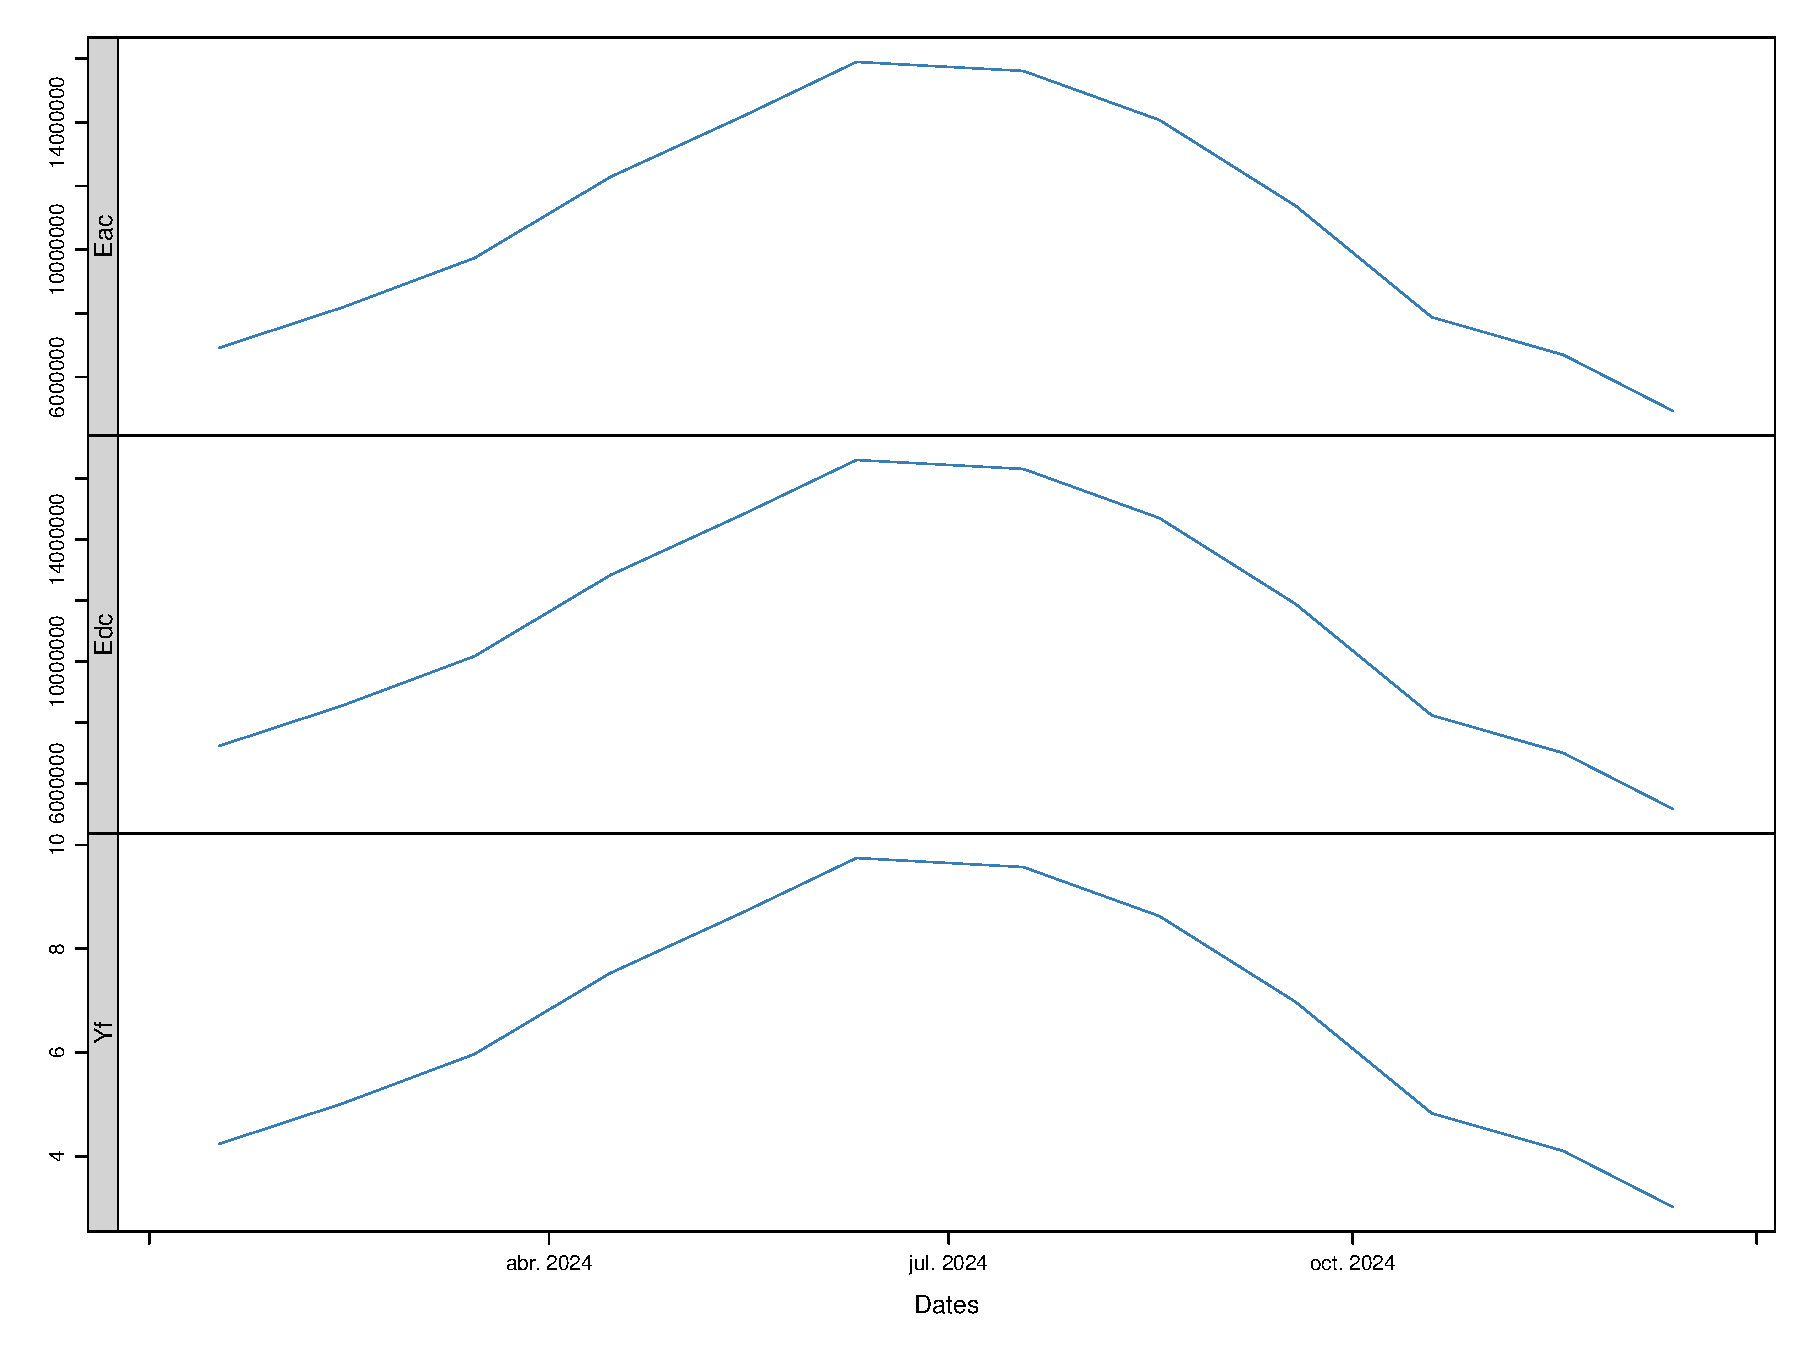
\includegraphics[width=0.8\textwidth]{figuras/codigo-prodgcpv.pdf}
\end{center}

Un método para \texttt{compare}.
\begin{lstlisting}[numbers=left,language=r,label= ,caption= ,captionpos=b]
prod2x <- prodGCPV(lat, modeTrk = 'two', dataRad = BD)
prodHoriz <- prodGCPV(lat, modeTrk = 'horiz', dataRad = BD)
compare(prodFixed, prod2x, prodHoriz)
\end{lstlisting}

\begin{center}
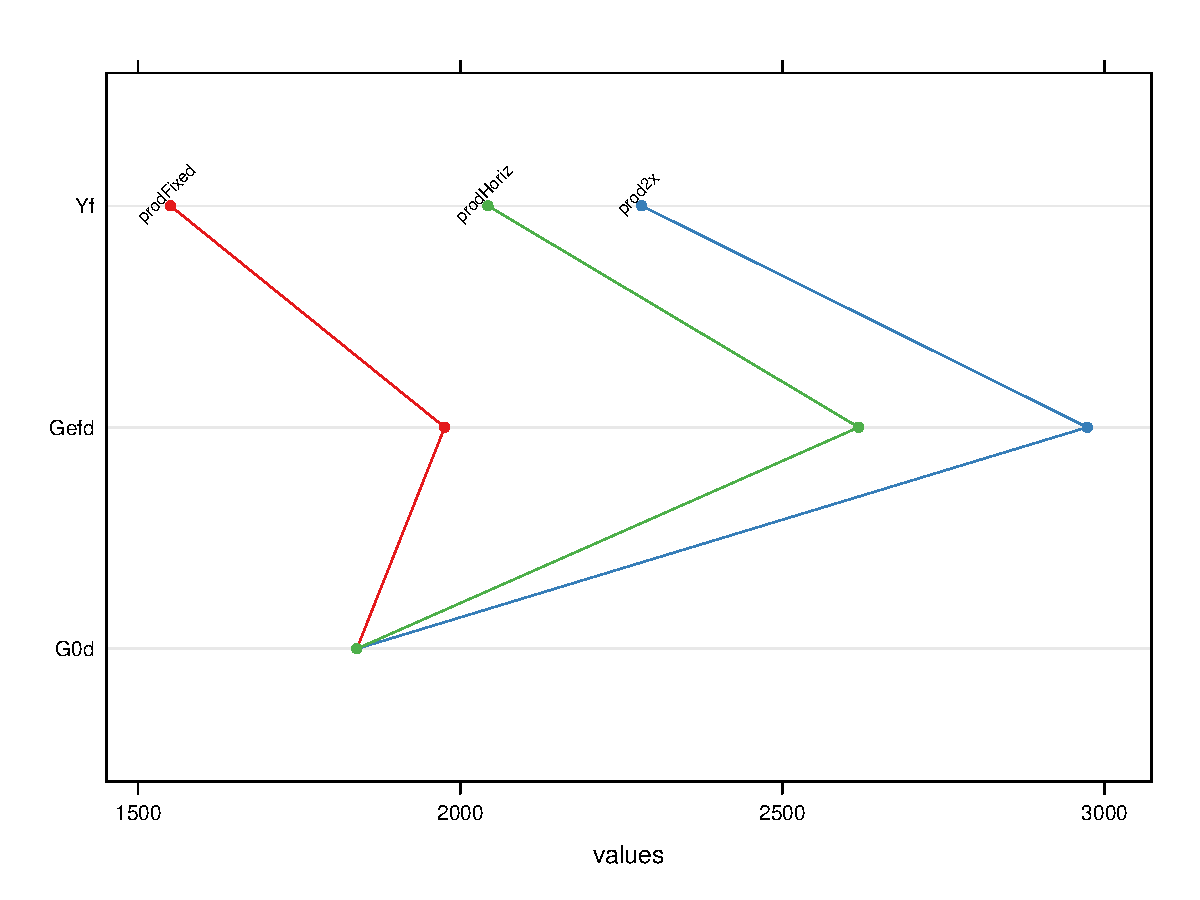
\includegraphics[width=0.8\textwidth]{figuras/codigo-prodgcpv2.pdf}
\end{center}

Y un método para \texttt{compareLosses}.
\begin{lstlisting}[numbers=left,language=r,label= ,caption= ,captionpos=b]
compareLosses(prodFixed, prod2x, prodHoriz)
\end{lstlisting}

\begin{center}
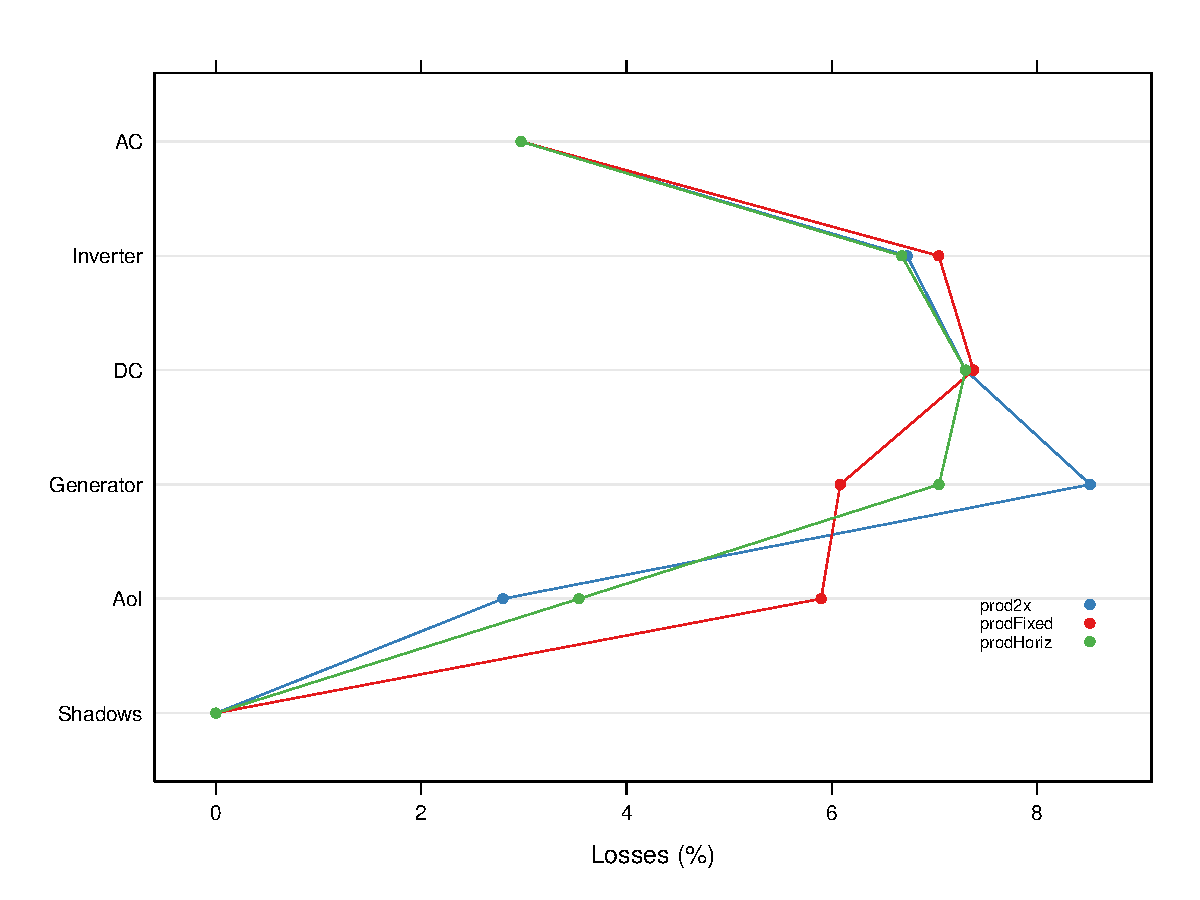
\includegraphics[width=0.8\textwidth]{figuras/codigo-prodgcpv3.pdf}
\end{center}

\subsection{Producción electrica de un SFB}
\label{sec:org4eaa4c7}
La clase \texttt{ProdPVPS} cuenta con un método para \texttt{xyplot}.
\begin{lstlisting}[numbers=left,language=r,label= ,caption= ,captionpos=b]
pump <- prodPVPS(lat, dataRad = BD, pump = CoefSP8A44, H = 40, Pg = 5000)
show(pump)
\end{lstlisting}

\begin{verbatim}
Object of class  ProdPVPS 

Source of meteorological information: prom- 

Latitude of source:  37.2 degrees
Latitude for calculations:  37.2 degrees

Monthly avarages:
        Dates      Eac       Qd       Yf
       <char>    <num>    <num>    <num>
 1: Jan. 2024 17.22642 59.71506 3.445284
 2: Feb. 2024 18.89837 64.60949 3.779675
 3: Mar. 2024 20.81307 70.36542 4.162613
 4: Apr. 2024 23.73937 79.08382 4.747874
 5: May. 2024 25.28080 83.74003 5.056160
 6: Jun. 2024 26.49158 87.02474 5.298315
 7: Jul. 2024 27.70317 89.81648 5.540633
 8: Aug. 2024 27.14273 87.89528 5.428546
 9: Sep. 2024 24.01466 79.04010 4.802932
10: Oct. 2024 18.26638 63.00860 3.653277
11: Nov. 2024 17.06794 59.03182 3.413588
12: Dec. 2024 13.72784 48.99686 2.745567

Yearly values:
   Dates      Eac       Qd       Yf
   <int>    <num>    <num>    <num>
1:  2024 7942.432 26608.76 1588.486
-----------------
Mode of tracking:  fixed 
    Inclination:  27.2 
    Orientation:  0 
-----------------
Pump:
    Qn:  8 
    Stages:  44 
Height (m):  40 
Generator (Wp):  5000
\end{verbatim}

\begin{lstlisting}[numbers=left,language=r,label= ,caption= ,captionpos=b]
xyplot(pump)
\end{lstlisting}

\begin{center}
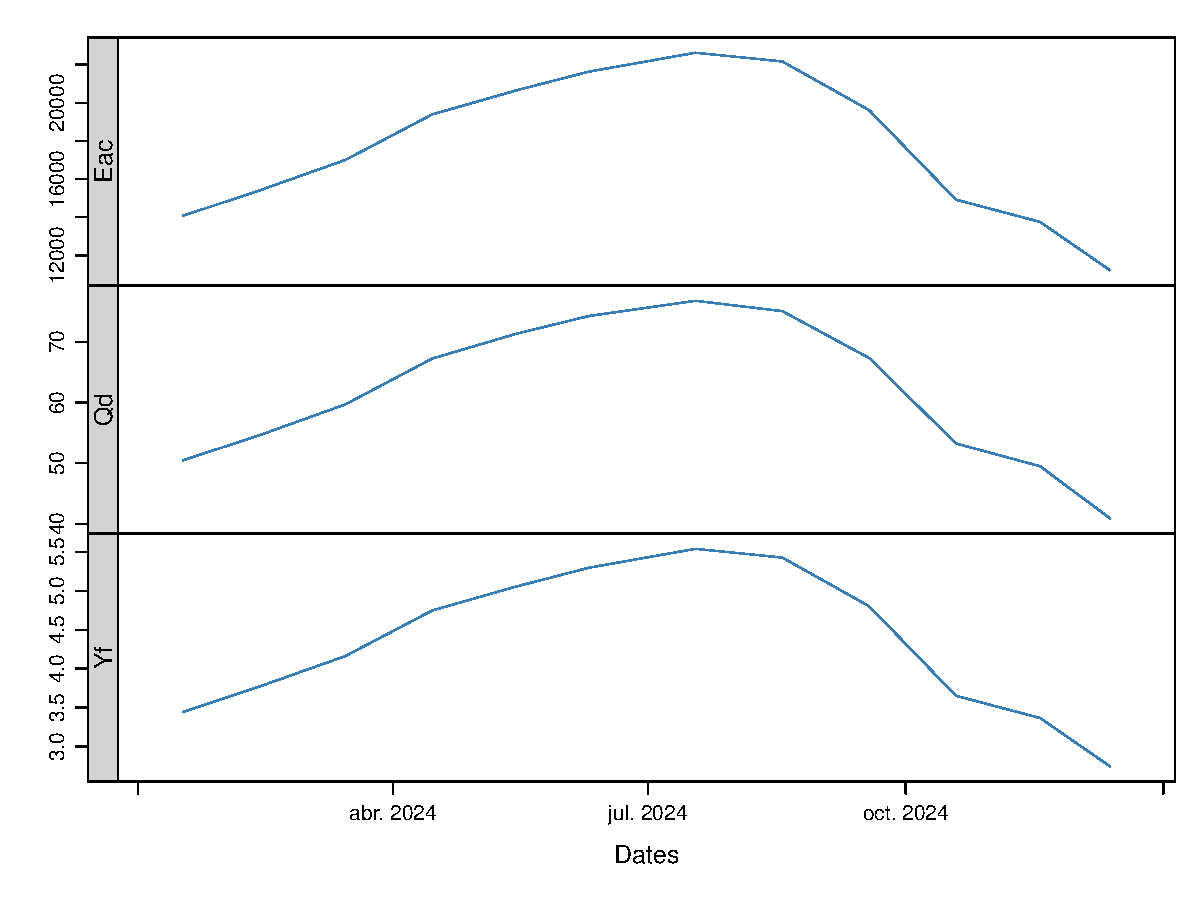
\includegraphics[width=.9\linewidth]{figuras/codigo-prodpvps.pdf}
\end{center}

\subsection{Optimización de distancias}
\label{sec:org00e6349}
La clase \texttt{Shade} cuenta con un método para \texttt{shadeplot}.
\begin{lstlisting}[numbers=left,language=r,label= ,caption= ,captionpos=b]
struct2x = list(W = 23.11, L = 9.8, Nrow = 2, Ncol = 3)
dist2x = list(Lew = c(30, 45),Lns = c(20, 40))
ShdM2x <- optimShd(lat = lat, dataRad = prom, modeTrk = 'two',
                    modeShd = c('area','prom'),
                   distances = dist2x, struct = struct2x,
                   res = 5, prog = FALSE)
show(ShdM2x)
\end{lstlisting}

\begin{verbatim}
Object of class  Shade 

Source of meteorological information: prom- 

Latitude of source:  37.2 degrees
Latitude for calculations:  37.2 degrees

Monthly avarages:
Dimensions of structure:
$W
[1] 23.11

$L
[1] 9.8

$Nrow
[1] 2

$Ncol
[1] 3

Shade calculation mode:
[1] "area" "prom"
Productivity without shadows:
Object of class  ProdGCPV 

Source of meteorological information: prom- 

Latitude of source:  37.2 degrees
Latitude for calculations:  37.2 degrees

Monthly avarages:
        Dates      Eac      Edc       Yf
       <char>    <num>    <num>    <num>
 1: Jan. 2024 138.6806 153.2566 5.241314
 2: Feb. 2024 143.4987 158.5247 5.423408
 3: Mar. 2024 151.8477 167.7311 5.738952
 4: Apr. 2024 178.6717 197.4274 6.752741
 5: May. 2024 200.8888 222.0523 7.592419
 6: Jun. 2024 223.9959 247.6903 8.465728
 7: Jul. 2024 214.2749 236.9628 8.098332
 8: Aug. 2024 194.6043 215.1439 7.354902
 9: Sep. 2024 168.9824 186.7349 6.386542
10: Oct. 2024 132.2995 146.0747 5.000145
11: Nov. 2024 128.5783 141.9871 4.859507
12: Dec. 2024 102.9116 113.5613 3.889454

Yearly values:
   Dates      Eac      Edc       Yf
   <int>    <num>    <num>    <num>
1:  2024 60369.04 66710.67 2281.595
-----------------
Mode of tracking:  two 
    Inclination limit: 90 
-----------------
Generator:
    Modules in series:  12 
    Modules in parallel:  11 
    Nominal power (kWp):  26.5 

Summary of results:
      Lew             Lns           H           FS               GRR              Yf      
 Min.   :30.00   Min.   :20   Min.   :0   Min.   :0.01509   Min.   :2.649   Min.   :2104  
 1st Qu.:33.75   1st Qu.:25   1st Qu.:0   1st Qu.:0.02223   1st Qu.:3.946   1st Qu.:2192  
 Median :37.50   Median :30   Median :0   Median :0.02870   Median :4.802   Median :2216  
 Mean   :37.50   Mean   :30   Mean   :0   Mean   :0.03463   Mean   :4.967   Mean   :2203  
 3rd Qu.:41.25   3rd Qu.:35   3rd Qu.:0   3rd Qu.:0.03945   3rd Qu.:6.016   3rd Qu.:2231  
 Max.   :45.00   Max.   :40   Max.   :0   Max.   :0.07769   Max.   :7.948   Max.   :2247
\end{verbatim}

\begin{lstlisting}[numbers=left,language=r,label= ,caption= ,captionpos=b]
shadeplot(ShdM2x)
\end{lstlisting}

\begin{center}
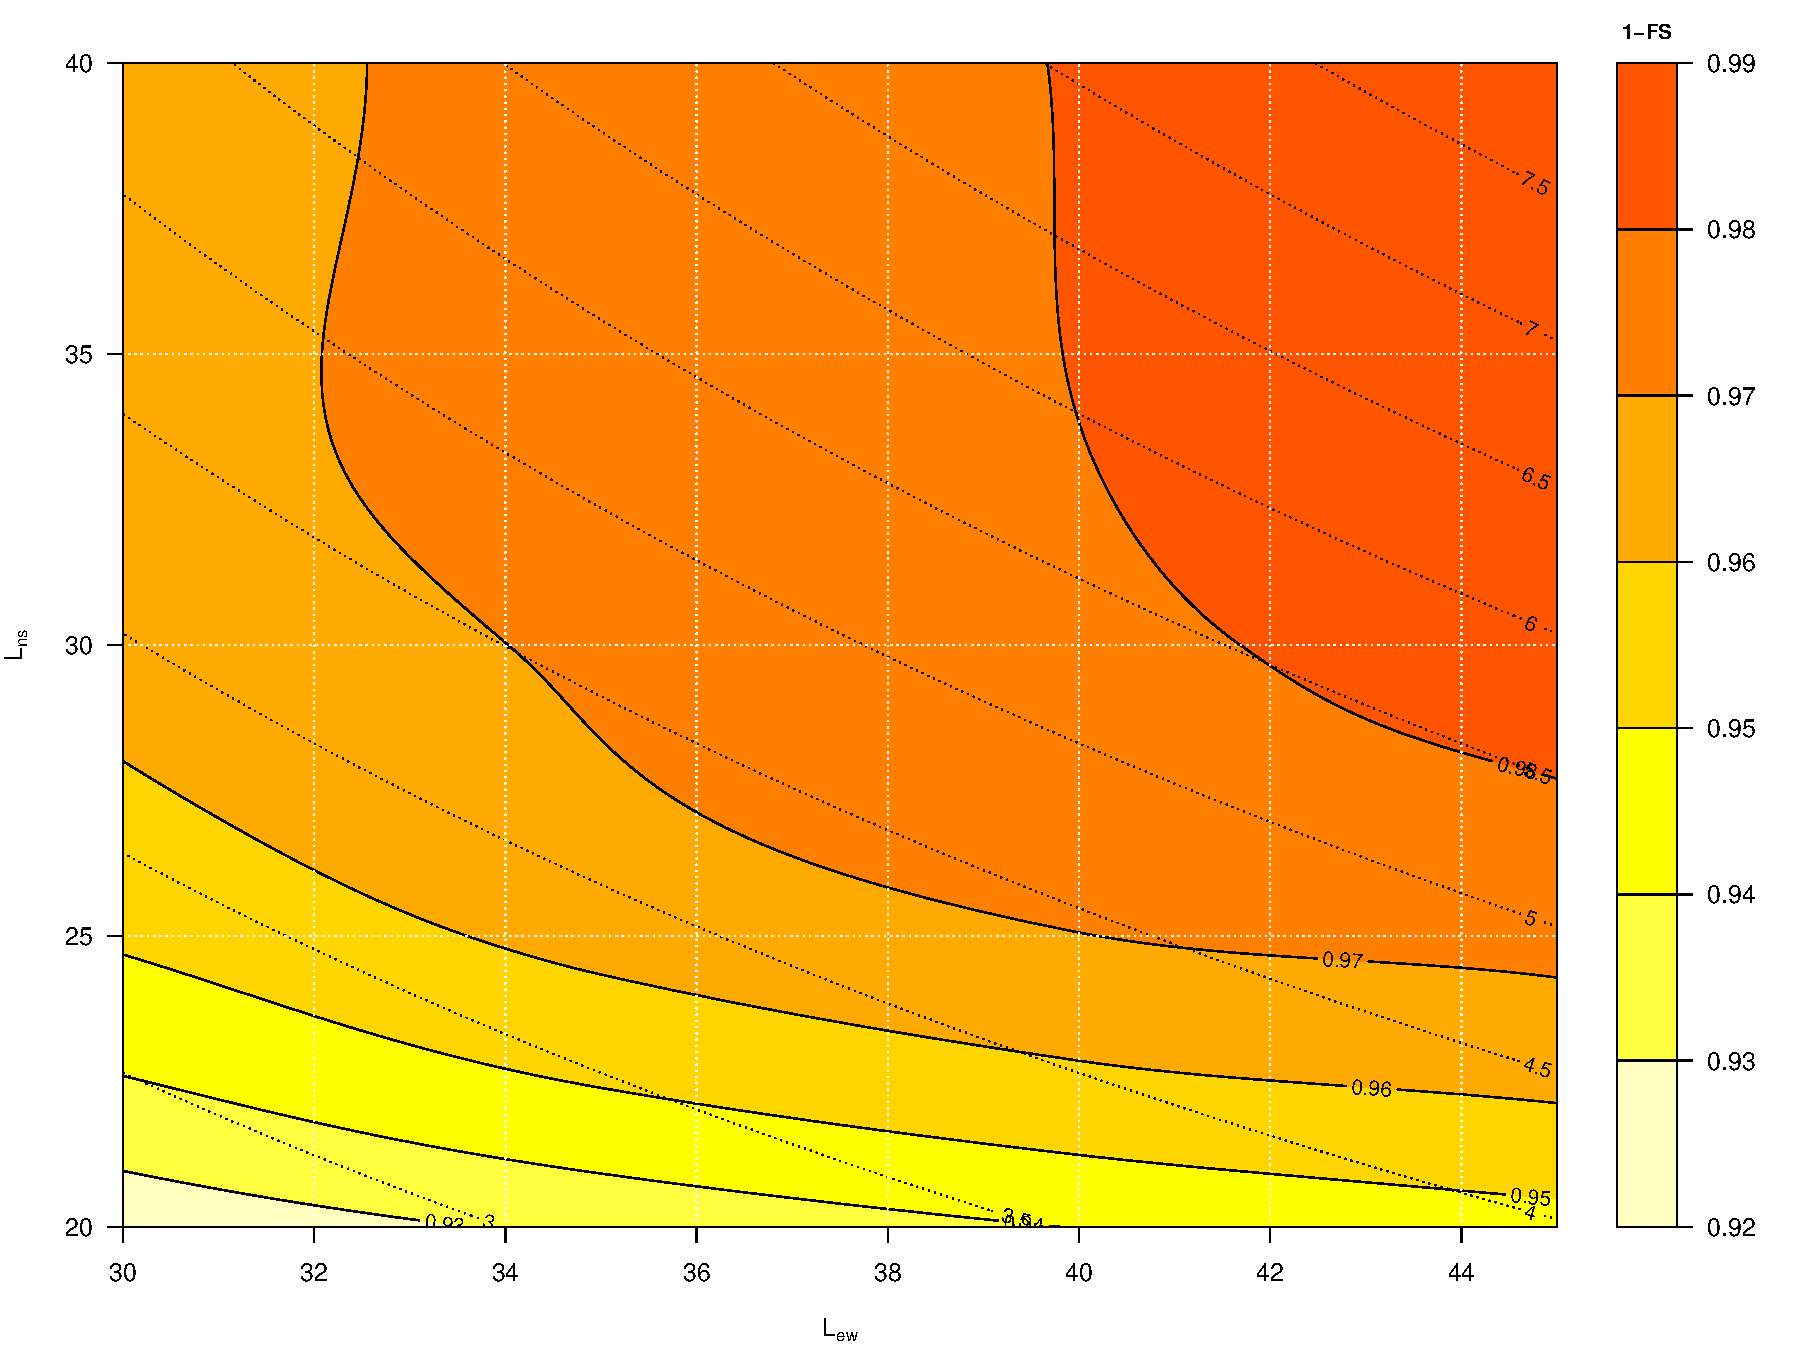
\includegraphics[width=0.8\textwidth]{figuras/codigo-optimshd.pdf}
\end{center}
